\documentclass[11pt]{article}

% PACKAGE IMPORTS
\usepackage{fancyhdr}
\usepackage[utf8]{inputenc}
\usepackage[T1]{fontenc}
\usepackage[english]{babel}
\usepackage{graphicx}
\usepackage{enumitem}
\usepackage{xcolor}
\usepackage{amsmath,amssymb}
\usepackage{booktabs}
\usepackage{tabularx}
\usepackage{array}
\usepackage{float}
\usepackage[font=small,skip=4pt]{caption}
\usepackage{subcaption}
\usepackage{geometry}
\usepackage{lastpage}
\usepackage[scaled]{helvet}
\usepackage{siunitx}
\sisetup{detect-all}
\PassOptionsToPackage{obeyspaces,spaces}{url}
\usepackage{hyperref}
\hypersetup{hidelinks}
\usepackage{url}
\usepackage{tikz} % Used for positioning text on title
\usepackage{eso-pic}
\usepackage[useregional]{datetime2}

% FIGURES: generated plots and screenshots in figures/, Fluent pictures of the runs in ../studyA/plots/
\graphicspath{{pictures/template/}{figures/}{../studyA/plots/}}

% FONT SETTINGS
\renewcommand\familydefault{\sfdefault}

% COLORS
\definecolor{ertred}{RGB}{226,12,24}

% MARGINS
\geometry{
a4paper,
inner=20mm,
outer=20mm,
top=26mm,
bottom=30mm,
footskip=10mm,
headsep=13mm
}

% LISTS, PATHS AND GUI NAMES
\setlength{\emergencystretch}{2em} % long paths and GUI names: stretch spaces rather than overflow
\setlist{itemsep=2pt,topsep=3pt}
\setlist[enumerate,1]{leftmargin=*}
\setlist[itemize]{leftmargin=*}
\urlstyle{tt}
\newcommand{\file}[1]{\path{#1}}
\newcommand{\zone}[1]{\texttt{#1}}              % Fluent zone / named selection
\newcommand{\gui}[1]{\textbf{#1}}               % menu, panel or field of the Ansys GUI
\newcommand{\then}{\,$\rightarrow$\,}           % menu path separator
\newcommand{\checkstep}[1]{\par\smallskip\noindent\textbf{Check.} #1\par\smallskip}

% PICTURE STILL TO COME FROM THE ANSYS SESSION: shown if figures/<name>.png exists, else a placeholder box
\newcommand{\shot}[3][\linewidth]{%
\IfFileExists{figures/#2.png}{\includegraphics[width=#1]{#2.png}}{%
\fbox{\parbox[c][3cm][c]{\dimexpr#1-2\fboxsep-2\fboxrule\relax}{\centering\small
\texttt{\detokenize{#2}.png} to come\\[2pt] #3}}}}

% FRONT PAGE BACKGROUND IMAGE
\newcommand\BackgroundPic{
\put(0,0){
\parbox[b][\paperheight]{\paperwidth}{
\vfill
\centering

\includegraphics[width=\paperwidth,height=\paperheight]{pictures/template/c_title-page.png} % Background title page image
\vfill
}
}
}

\begin{document}

\AddToShipoutPicture*{\BackgroundPic}
\ClearShipoutPicture

% HEADER AND FOOTER
\let\oldheadrule\headrule
\renewcommand{\headrule}{\color{ertred}\oldheadrule}
\renewcommand{\headrulewidth}{1.5pt}
\renewcommand{\footrule}{\hbox to\headwidth{\color{ertred}\leaders\hrule height \footrulewidth\hfill}}
\renewcommand{\footrulewidth}{1.5pt}
\setlength\headheight{48pt}

\pagestyle{fancy}
\fancyhead[C]{\rule[-2ex]{0pt}{2ex} \bf{\fontsize{12}{5}\selectfont 2027\_C\_FD\_REPORT-4\_NOSE-CONE-FLUENT-WORKFLOW}}
\lhead{
\includegraphics[height=1.5cm]{ert_logo_small}\vspace{-4mm}}
\rhead{
\includegraphics[height=1.5cm]{c_patch.png}\vspace{-4mm}}
\cfoot{}
\fancyfoot[R]{\bf{\thepage/\pageref{LastPage}}}
\fancyfoot[L]{\rule[-2ex]{0pt}{2ex}\bf{EPFL ROCKET TEAM}}

% TITLE PAGE
\begin{titlepage}
\vspace*{-2.40cm} % Push title to the top of the page
\noindent
\hspace*{-1.2cm}
\parbox{\linewidth}{%
\bfseries\fontsize{34}{38}\selectfont
REPORT 4 -\\
NOSE CONE CFD\\
IN ANSYS FLUENT\\
}
\newline
\hspace*{-1.2cm}
\parbox{\linewidth}{%
\bfseries\fontsize{14}{18}\selectfont
Fabio Feig - 315169 \\ % Names and scipers
}

% ADDITIONAL TITLE PAGE DETAILS
\begin{tikzpicture}[remember picture,overlay]
\node[anchor=south east,inner sep=39mm] at (current page.south east) {
\parbox[b][-2.37cm][t]{15cm}{
\raggedleft
\fontsize{12}{12} \selectfont \normalfont \textbf{Weisshorn -- Nose Cone CFD: Workflow and Study A}
}
};
\end{tikzpicture}

\begin{tikzpicture}[remember picture,overlay]
\node[anchor=south east,inner sep=39mm] at (current page.south east) {
\parbox[b][-1.6cm][t]{15cm}{
\raggedleft
\fontsize{12}{12} \selectfont \normalfont Doc ID: 2027\_C\_FD\_REPORT-4\_NOSE-CONE-FLUENT-WORKFLOW
}
};
\end{tikzpicture}

\begin{tikzpicture}[remember picture,overlay]
\node[anchor=south east,inner sep=39mm] at (current page.south east) {
\parbox[b][-0.8cm][t]{15cm}{
\raggedleft
\fontsize{12}{12} \selectfont \normalfont Date: \today % Date
}
};
\end{tikzpicture}

\end{titlepage}

% TABLE OF CONTENTS
\pagenumbering{roman} % front matter numbered i, ii so the report body starts at 1
\setcounter{tocdepth}{2} % sections and subsections only
{\small\tableofcontents}
\newpage

% PAGE NUMBERING
\pagenumbering{arabic}
\setcounter{page}{1}

% MAIN CONTENT
\section{Summary}
\label{sec:summary}

Fluent workflow for the Weisshorn nose cone, written as the step-by-step record of study~A of
2027\_C\_FD\_REPORT-2\_NOSE-CONE-650MM: LV-Haack, \SI{561}{mm} curved part + \SI{89}{mm} coupler,
$D = \SI{180}{mm}$, $r_n = \SI{4.5}{mm}$, zero incidence. Steady 2D axisymmetric RANS (k-$\omega$ SST) in
Fluent 2024~R2 at $M = 0.95$, 1.2 and 1.47. Sections~\ref{sec:geometry}--\ref{sec:runs}: steps;
Section~\ref{sec:results}: results; Section~\ref{sec:python}: comparison with Python. Study~B will be
added after its runs.

\begin{table}[H]
\centering
\caption{Study~A: drag coefficient of the nose (\zone{wall\_nose}, tip to shoulder),
$A_{\rm ref} = \pi D^2/4 = \SI{0.02545}{m^2}$.}
\label{tab:summary}
\small
\begin{tabular}{@{}lrrr@{}}
\toprule
 & $M = 0.95$ & $M = 1.2$ & $M = 1.47$ \\
\midrule
Pressure $C_D$ & 0.0042 & 0.0948 & 0.0963 \\
Viscous $C_D$ & 0.0248 & 0.0224 & 0.0207 \\
\textbf{Total $C_D$} & \textbf{0.0291} & \textbf{0.1172} & \textbf{0.1170} \\
Drag force & \SI{42.3}{N} & \SI{254.8}{N} & \SI{349.4}{N} \\
Solver & pressure-based & density-based & density-based \\
\bottomrule
\end{tabular}
\end{table}

\begin{itemize}
\item \textbf{Supersonic}: $C_D \approx 0.117$, four fifths of it wave drag. Density-based with Roe-FDS,
about 3000 iterations.
\item \textbf{Transonic}: pressure drag $\approx 0$, friction 85\,\% of the total. Only the pressure-based
Coupled solver converged.
\item \textbf{Against Python}: wave drag $+2.4\,\%$, friction within 5\,\%. The transonic ramp gives 0.077
where Fluent gives 0.004, so the report-2 drag is conservative below $M = 1$.
\end{itemize}

\section{Case definition}
\label{sec:case}

\subsection{The noses}

\begin{table}[H]
\centering
\caption{The two noses of report~2. Lengths in mm; $x$ is measured from the rounded tip.}
\label{tab:noses}
\small
\begin{tabular}{@{}lll@{}}
\toprule
 & Study A (this report) & Study B (to be run) \\
\midrule
Profile & LV-Haack & Von K\'arm\'an \\
Nominal curved length $L$, fineness $L/D$ & 561, 3.117 & 630, 3.5 \\
Coupler length $c$, total length & 89, 650 & 20, 650 \\
Tip radius $r_n$ & 4.5 & 4.5 \\
End of the curved part (shoulder), $x$ & 558.65 & 625.42 \\
End of the coupler, $x$ & 647.65 & 645.42 \\
\bottomrule
\end{tabular}
\end{table}

\noindent Both noses are solids of revolution in mm, with $x$ along the axis and the tip at $x = 0$. The
\SI{4.5}{mm} tip rounding shortens the curved part by \SI{2.35}{mm} (A) and \SI{4.58}{mm} (B). STEP files:
\file{CFD/geometry_650/nose_lvhaack_L561_c89_rn4.5mm.step} (A),
\file{nose_vonkarman_L630_c20_rn4.5mm.step} (B).

\subsection{Flight conditions}

\begin{table}[H]
\centering
\caption{Flight conditions of the three runs (altitude above sea level).}
\label{tab:points}
\small
\begin{tabular}{@{}rrrrl@{}}
\toprule
$M$ & altitude & $p_\infty$ & $T_\infty$ & type of flow \\
\midrule
0.95 & \SI{928}{m}  & \SI{90666}{Pa} & \SI{282.1}{K} & transonic: just below the speed of sound \\
1.20 & \SI{1478}{m} & \SI{84789}{Pa} & \SI{278.5}{K} & supersonic, close to $M = 1$ \\
1.47 & \SI{2189}{m} & \SI{77649}{Pa} & \SI{273.9}{K} & supersonic, top speed of the flight \\
\bottomrule
\end{tabular}
\end{table}

\noindent The inputs are $M$, $p_\infty$ and $T_\infty$, from the report-1 trajectory. On the report-2
trajectory of nose~A the same Mach numbers are reached within \SI{14}{m} of altitude and 0.2\,\% in
pressure; its top speed is $M = 1.457$ (\SI{2182}{m}), so the $M = 1.47$ run is the top-speed point
($+1\,\%$).

\paragraph{Why the speed matters.} Pressure waves travel upstream at the speed $a - V$ relative to the
rocket:
\begin{itemize}
\item $M < 1$: $a - V > 0$, the air ahead feels the nose coming. No bow shock; a small supersonic zone
forms at the shoulder and ends in a weak shock (transonic flow).
\item $M > 1$: $a - V < 0$, the air ahead is undisturbed until a bow shock just in front of the tip. The
high pressure behind it, acting on the front of the nose, is the wave drag.
\end{itemize}

\paragraph{What the runs give.} The drag on \zone{wall\_nose} (tip to shoulder), split by Fluent into
pressure and viscous parts:
\begin{equation}
C_D = \frac{F_x}{q_\infty A_{\rm ref}}, \qquad q_\infty = \tfrac12\rho_\infty V_\infty^2, \qquad
A_{\rm ref} = \frac{\pi D^2}{4}.
\end{equation}

\subsection{Symbols}

\begin{small}
\noindent
$a$ speed of sound; $A_{\rm ref}$ reference area $\pi D^2/4$; $C_D$ drag coefficient; $C_f$ friction
coefficient; $C_p$ pressure coefficient; CFL Courant number; $c_p$ specific heat at constant pressure; $D$
body diameter (\SI{180}{mm}); $F_x$ force along the rocket axis; $h_1$ height of the first cell at the
wall; $I$ turbulence intensity; $k$ turbulent kinetic energy; $M$ Mach number; $p$ pressure; $T_0$
stagnation (total) temperature; $q = \tfrac12\rho V^2$ dynamic pressure; $R$ gas constant of
air; $\mathrm{Re}$ Reynolds number; $r_n$ tip radius; $T$ temperature; $u_\tau$ friction velocity; $V$
flow speed; $y^+$ wall distance in viscous units; $\gamma$ ratio of specific heats; $\delta$
boundary-layer thickness; $\mu$ viscosity of the air; $\mu_t$ turbulent (eddy) viscosity; $\rho$
density; $\tau_w$ wall shear stress; $\omega$ turbulence frequency (specific dissipation rate).
Subscript $\infty$: the undisturbed air far from the rocket (free stream).
\end{small}

\section{Step 1: Geometry}
\label{sec:geometry}

The flow domain is a flat rectangle in the $xy$ plane, above the rocket axis ($y \geq 0$), with the
outline of the nose cut out of its lower edge (Figure~\ref{fig:domain}). It is built in Discovery, inside
Workbench, from the design STEP file.

\subsection{Steps}

\begin{enumerate}
\item \textbf{Workbench.} Add a \gui{Fluid Flow (Fluent)} system. Before importing anything, click the
\gui{Geometry} cell and set \gui{Properties}\then\gui{Analysis Type} = \gui{2D}. Without this setting,
Fluent does not offer the axisymmetric option used below.
\item \textbf{Import.} \gui{Geometry}\then\gui{Import Geometry}\then\gui{Browse}, choose
\file{CFD/geometry_650/nose_lvhaack_L561_c89_rn4.5mm.step} and open it in \gui{Discovery}
(Figure~\ref{fig:geom-step}). Use the STEP file, not the STL: the STL is made of small flat triangles,
and cutting, naming edges and meshing do not work cleanly on it.
\item \textbf{Extend the body.} With \gui{Pull}, drag the flat end face of the coupler by
\SI{+1800}{mm}, from $x = \SI{647.65}{mm}$ to $x = \SI{2447.65}{mm}$. The body is now a long cylinder
that reaches the end of the domain.
\item \textbf{Draw the domain.} In the $XY$ plane, sketch the rectangle from $x = -3600$, $y = 0$ to
$x = 2447.65$, $y = 3600$ (mm) and turn it into a surface.
\item \textbf{Cut out the body.} \gui{Combine}\then\gui{Subtract from target}: the rectangle is the
target, the solid is the tool that cuts. Delete the solid and any piece left inside the body. One
surface remains, with the half-outline of the nose along its lower edge (Figure~\ref{fig:geom-domain}).
The nose and cylinder edges are already separate, because they are separate faces in the STEP file.
\item \textbf{Save the project} (\gui{File}\then\gui{Save As}). Until it is saved, Workbench keeps the
geometry in a temporary folder and loses it if it restarts. The study-A domain is stored as
\file{CFD/geometry_650/studyA_domain2D_2024R2.dsco}.
\item \textbf{Name the edges.} In Meshing, select each edge, right-click\then\gui{Create Named
Selection}, and use exactly the names of Table~\ref{tab:named}. Fluent turns them into boundaries with
the same names, and the boundary conditions of Step~3 are set on them (Figure~\ref{fig:geom-named}). A
typing error (\zone{wal\_nose}) means renaming the zone in Fluent later.
\end{enumerate}

\begin{table}[H]
\centering
\caption{Named edges of the study-A domain (Figure~\ref{fig:domain}).}
\label{tab:named}
\small
\begin{tabular}{@{}lll@{}}
\toprule
Name & Edge & Position [m] \\
\midrule
\zone{inlet} & left (upstream) edge & $x = -3.6$, $y$ from 0 to 3.6 \\
\zone{farfield} & top edge & $y = 3.6$, $x$ from $-3.6$ to 2.44765 \\
\zone{outlet} & right (downstream) edge & $x = 2.44765$, $y$ from 0.09 to 3.6 \\
\zone{axis} & rocket axis in front of the tip & $y = 0$, $x$ from $-3.6$ to 0 \\
\zone{wall\_nose} & curved nose, rounded tip included & $x$ from 0 to 0.55865 \\
\zone{wall\_body} & cylinder: coupler and its extension & $y = 0.09$, $x$ from 0.55865 to 2.44765 \\
\bottomrule
\end{tabular}
\end{table}

\checkstep{The surface lies entirely above the axis ($y \geq 0$), the $x$ axis is the rocket axis, the
tip is at the origin, and every edge has exactly one name. When the mesh is read into Fluent, the console
lists one fluid zone and these six boundaries.}

\subsection{Why the domain looks like this}

\begin{figure}[H]
\centering
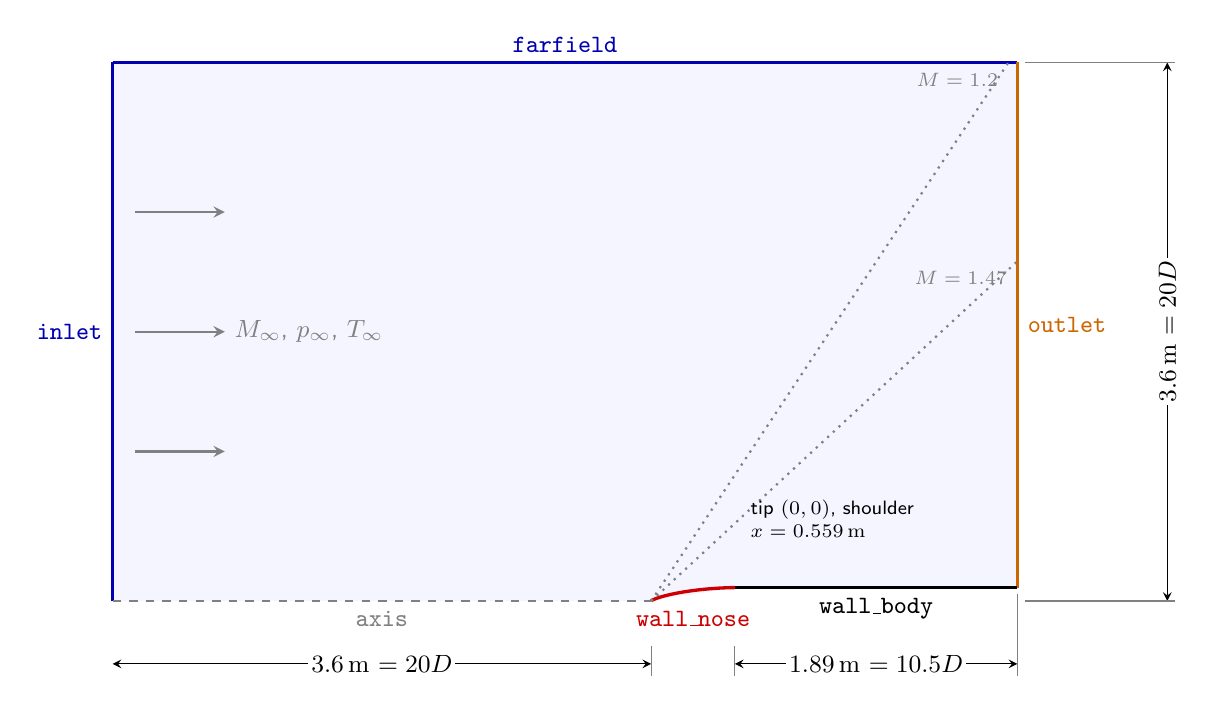
\begin{tikzpicture}[x=1.9cm,y=1.9cm,>=stealth,font=\small]
  % domain, to scale (x from -3.6 to 2.448 m, y from 0 to 3.6 m)
  \fill[blue!4] (-3.6,0) -- (0,0) -- (0.559,0.09) -- (2.448,0.09) -- (2.448,3.6) -- (-3.6,3.6) -- cycle;
  \draw[thick,blue!70!black] (-3.6,0) -- (-3.6,3.6) node[midway,left,align=right] {\zone{inlet}};
  \draw[thick,blue!70!black] (-3.6,3.6) -- (2.448,3.6) node[midway,above] {\zone{farfield}};
  \draw[thick,orange!80!black] (2.448,0.09) -- (2.448,3.6) node[midway,right] {\zone{outlet}};
  \draw[thick,dashed,gray] (-3.6,0) -- (0,0) node[midway,below] {\zone{axis}};
  \draw[very thick,red!80!black] plot[domain=0:180,samples=40,variable=\t]
     ({0.559*(1-cos(\t))/2},{0.09/sqrt(pi)*sqrt(rad(\t)-sin(2*\t)/2+sin(\t)^3/3)});
  \draw[very thick,black] (0.559,0.09) -- (2.448,0.09) node[midway,below] {\zone{wall\_body}};
  \node[red!80!black,below] at (0.28,0) {\zone{wall\_nose}};
  % free stream
  \foreach \yy in {1.0,1.8,2.6} \draw[->,thick,gray] (-3.45,\yy) -- (-2.85,\yy);
  \node[gray,right] at (-2.85,1.8) {$M_\infty$, $p_\infty$, $T_\infty$};
  % dimensions
  \draw[<->] (-3.6,-0.42) -- (0,-0.42) node[midway,fill=white,inner sep=1pt] {\SI{3.6}{m} $= 20D$};
  \draw[<->] (0.559,-0.42) -- (2.448,-0.42) node[midway,fill=white,inner sep=1pt] {\SI{1.89}{m} $= 10.5D$};
  \draw[gray,thin] (0,-0.3) -- (0,-0.5) (0.559,-0.3) -- (0.559,-0.5) (2.448,0.05) -- (2.448,-0.5);
  \draw[<->] (3.45,0) -- (3.45,3.6) node[midway,fill=white,inner sep=1pt,rotate=90] {\SI{3.6}{m} $= 20D$};
  \draw[gray,thin] (2.5,3.6) -- (3.5,3.6) (2.5,0) -- (3.5,0);
  % weak-wave directions from the tip at M = 1.2 and 1.47
  \draw[gray,dotted,thick] (0,0) -- ({3.6/tan(56.44)},3.6) node[below left,font=\scriptsize] {$M = 1.2$};
  \draw[gray,dotted,thick] (0,0) -- (2.448,{2.448*tan(42.86)}) node[below left,font=\scriptsize] {$M = 1.47$};
  \node[font=\scriptsize,align=left,anchor=west] at (0.6,0.55) {tip $(0,0)$, shoulder\\$x = \SI{0.559}{m}$};
\end{tikzpicture}
\caption{Study-A flow domain to scale, with the named edges. The nose is the small bump on the lower
edge. Dotted: the direction in which the bow shock ends up far from the body, at the angle
$\arcsin(1/M)$.}
\label{fig:domain}
\end{figure}

\begin{itemize}
\item \textbf{Only a 2D half-plane (axisymmetric).} With no angle of attack the flow is the same in every
plane through the rocket axis, so the half-plane $y \geq 0$ is enough. Fluent counts each wall element as
a ring, $\mathrm dA = 2\pi y\,\mathrm ds$, and reports the forces of the full body.
\item \textbf{Far boundaries \SI{3.6}{m} ($20D$) ahead and above.} The undisturbed air is imposed there,
so the nose must have no effect at that distance. Above $M = 1$ the air ahead of the bow shock is
undisturbed anyway; below $M = 1$ the disturbance fades with distance, and $20D$ is the usual margin.
\item \textbf{Outlet \SI{1.89}{m} ($10.5D$) behind the shoulder.} Far enough for the flow along the
cylinder to settle before it leaves. Far from the body the bow shock lies at $\mu = \arcsin(1/M)$:
\SI{56.4}{\degree} at $M = 1.2$, \SI{42.9}{\degree} at $M = 1.47$ (dotted lines). At $M = 1.47$ it leaves
through the outlet; at $M = 1.2$ it reaches the top edge at $x = \SI{3.6}{m}/\tan\mu \approx \SI{2.4}{m}$,
where the far-field condition lets it out without reflection (Section~\ref{sec:bc}).
\item \textbf{The cylinder runs out of the domain.} A body ending inside the domain would have a flat base
with an unsteady wake, which a steady run cannot settle and which, below $M = 1$, also affects the nose.
Running the cylinder out gives the drag of the nose alone; its length is set by the domain, not by the
rocket.
\end{itemize}

\begin{figure}[H]
\centering
\begin{subfigure}[t]{0.48\linewidth}
\centering
\shot{geom_1_step}{design STEP in Discovery, isometric, before any edit}
\caption{Starting geometry: the design solid from the STEP file.}
\label{fig:geom-step}
\end{subfigure}\hfill
\begin{subfigure}[t]{0.48\linewidth}
\centering
\shot{geom_3_domain}{final 2D surface, whole domain}
\caption{Final geometry: the 2D flow domain after the cut, with the nose region enlarged.}
\label{fig:geom-domain}
\end{subfigure}
\caption{Geometry in Discovery (Ansys 2024~R2).}
\label{fig:geom}
\end{figure}

\begin{figure}[H]
\centering
\shot[0.85\linewidth]{geom_4_named_sel}{named selections in colour, whole domain and nose zoom}
\caption{The six named edges and the boundary type each one gets in Fluent, drawn from the boundary
zones of the Fluent mesh. Insert: the nose, where \zone{wall\_nose} ends and \zone{wall\_body} starts.}
\label{fig:geom-named}
\end{figure}

\section{Step 2: Mesh}
\label{sec:mesh}

The mesh is made in Ansys Meshing 2024~R2. Close to the two walls it has thin quadrilateral inflation
layers to capture the boundary layer; the rest of the domain is filled with triangles, made smaller
along the nose and at the tip (Figure~\ref{fig:mesh}).

\subsection{Steps}

\begin{enumerate}
\item Open the \gui{Mesh} cell. In \gui{Mesh}\then\gui{Details}: \gui{Physics Preference} = CFD,
\gui{Solver Preference} = Fluent, \gui{Element Order} = Linear, \gui{Element Size} = \SI{0.05}{m},
\gui{Growth Rate} = 1.1, \gui{Smoothing} = High.
\item \gui{Insert}\then\gui{Method} on the surface: triangles. A quadrilateral-dominant fill failed on
this surface.
\item \gui{Insert}\then\gui{Sizing} on edges: \zone{wall\_nose} \SI{1}{mm}; \zone{wall\_body}
\SI{1}{mm} with \gui{Bias Type} towards the shoulder and \gui{Bias Factor} = 3, so the cells are small at
the shoulder and grow towards the outlet.
\item \gui{Insert}\then\gui{Sizing} on the surface, \gui{Type} = \gui{Sphere of Influence}: centre at
the origin (the tip), radius \SI{15}{mm}, element size \SI{0.2}{mm}.
\item \gui{Insert}\then\gui{Inflation} on the surface, boundary = \zone{wall\_nose} and
\zone{wall\_body}: \gui{Inflation Option} = \gui{First Layer Thickness}, first layer
\SI{1}{\micro m}, 45 layers, growth rate 1.2, \gui{Collision Avoidance} = \gui{Layer Compression}.
\item \gui{Generate}, then look at the quality: \gui{Mesh}\then\gui{Quality}\then\gui{Mesh Metric} =
\gui{Skewness}, then \gui{Orthogonal Quality} (Section~\ref{sec:quality}). Close Meshing and
\gui{Update} the Mesh cell so that Fluent receives the mesh with the named selections.
\end{enumerate}

\checkstep{Maximum skewness below 0.95 and minimum orthogonal quality well above 0.01; in Fluent,
\gui{Domain}\then\gui{Mesh}\then\gui{Check} passes with no negative volumes. The study-A mesh has
169\,674 cells (Table~\ref{tab:mesh}).}

\begin{table}[H]
\centering
\caption{Study-A mesh.}
\label{tab:mesh}
\small
\begin{tabular}{@{}ll@{}}
\toprule
Cells & 169\,674 \\
Faces / nodes & 312\,923 / 143\,250 \\
Faces on \zone{wall\_nose} / \zone{wall\_body} & 639 / 1889 \\
Faces on \zone{axis} / \zone{inlet} / \zone{farfield} / \zone{outlet} & 205 / 72 / 121 / 138 \\
\midrule
Maximum skewness (Meshing) & 0.92 \\
Minimum orthogonal quality (Meshing / Fluent) & 0.237 / 0.077 \\
Maximum aspect ratio & 1660 (first inflation layer at the shoulder) \\
Fluent mesh check & passed, no negative volumes \\
\bottomrule
\end{tabular}
\end{table}

\begin{figure}[H]
\centering
\begin{subfigure}[t]{0.49\linewidth}
\centering
\shot{mesh_1_full}{whole domain}
\caption{Whole domain.}
\end{subfigure}\hfill
\begin{subfigure}[t]{0.49\linewidth}
\centering
\shot{mesh_2_nose}{nose and shoulder}
\caption{Nose and shoulder.}
\end{subfigure}

\medskip
\begin{subfigure}[t]{0.49\linewidth}
\centering
\shot{mesh_3_tip}{tip, about 20 mm window}
\caption{Tip, about \SI{20}{mm} window: inflation layers around the rounded tip.}
\label{fig:mesh-tip}
\end{subfigure}\hfill
\begin{subfigure}[t]{0.49\linewidth}
\centering
\shot{mesh_4_inflation}{inflation layers at the shoulder, about 5 mm window}
\caption{Inflation layers at the shoulder, about \SI{5}{mm} window.}
\end{subfigure}
\caption{Study-A mesh, as read by Fluent.}
\label{fig:mesh}
\end{figure}

\subsection{Why these sizes}

\paragraph{First cell height.} SST is solved down to the wall, without wall functions, so the first cell
must sit in the viscous layer: $y^+ = \rho u_\tau y/\mu \approx 1$. Flat-plate estimate at the shoulder
($x = \SI{0.559}{m}$), with the free stream of Section~\ref{sec:freestream}:
\begin{equation}
\mathrm{Re}_x = \frac{\rho V x}{\mu}, \qquad
C_f \approx 0.026\,\mathrm{Re}_x^{-1/7}, \qquad
u_\tau = V\sqrt{\frac{C_f}{2}}, \qquad
h_1 = \frac{y^+\,\mu}{\rho\,u_\tau}\bigg|_{y^+ = 1}.
\label{eq:y1}
\end{equation}
This gives $h_1 = 1.38$, 1.16 and \SI{1.02}{\micro m} at $M = 0.95$, 1.2 and 1.47, so one mesh with
$h_1 = \SI{1}{\micro m}$ covers all three. Fluent's $y^+$ after the runs stays below 0.71 on the nose and
0.30 on the cylinder (Figure~\ref{fig:yplus}).

\begin{figure}[H]
\centering
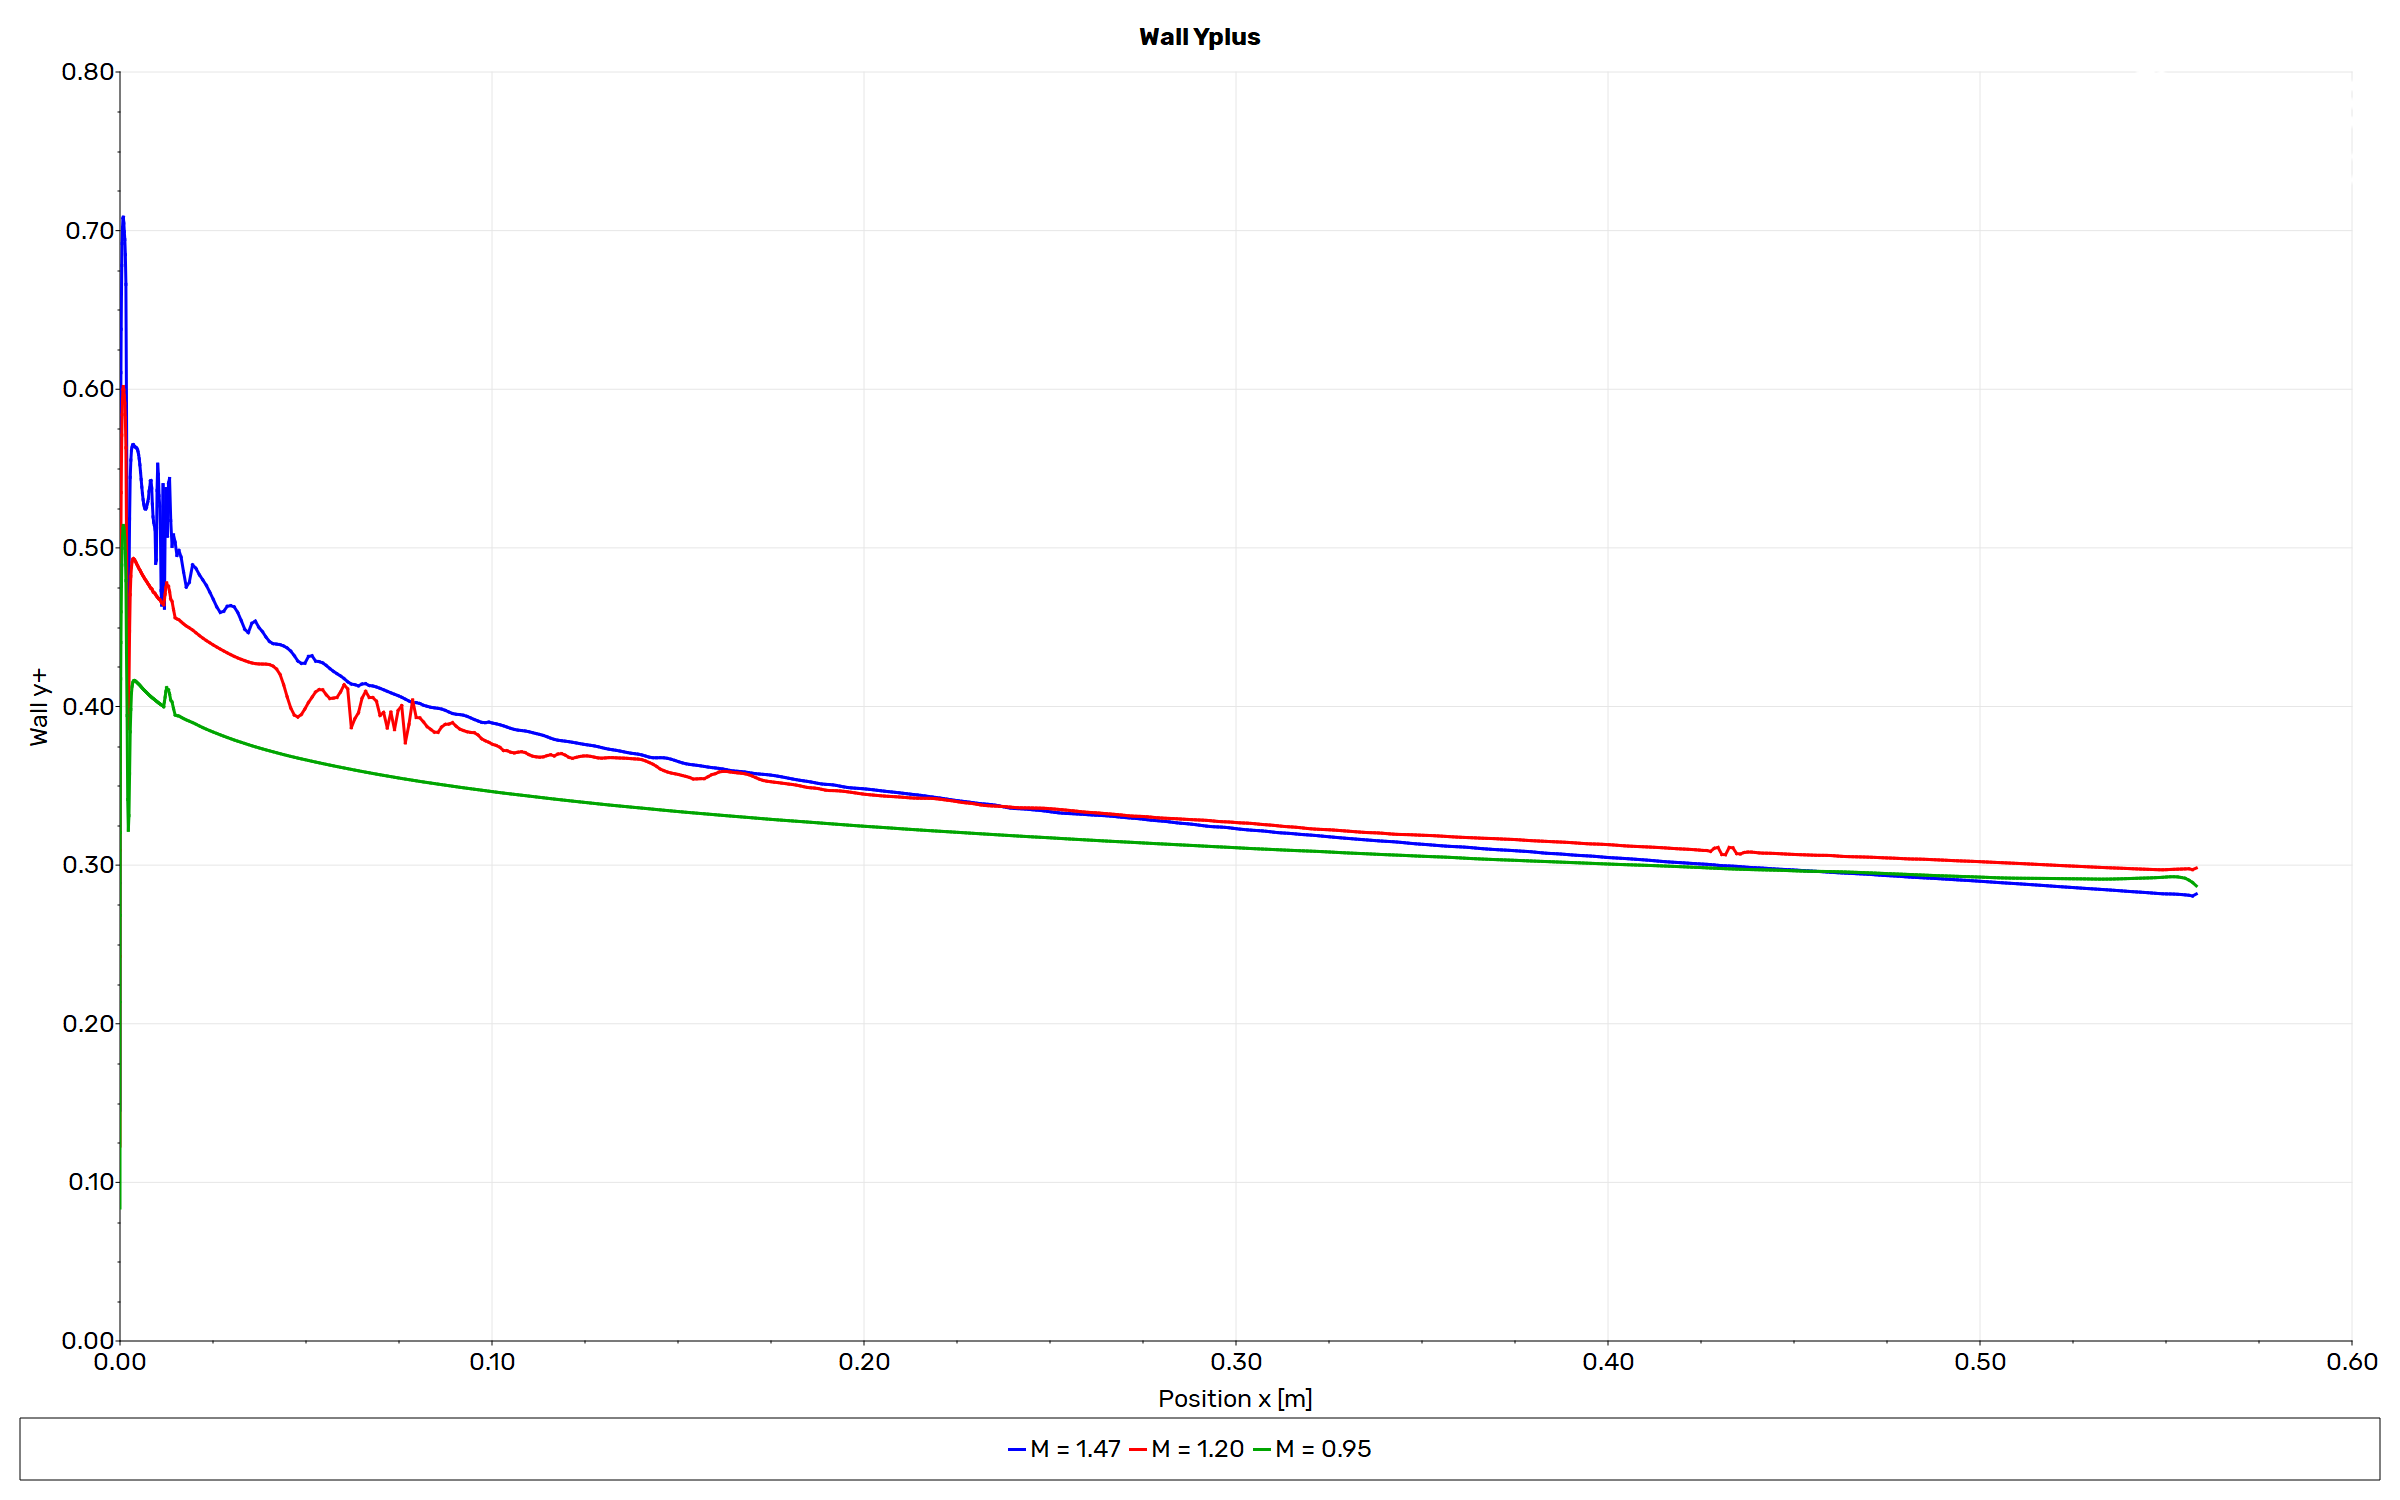
\includegraphics[width=0.9\linewidth]{fluent_yplus_all}
\caption{Wall $y^+$ along \zone{wall\_nose} at the three Mach numbers (Fluent XY plot). It stays below
1 everywhere, as Equation~\eqref{eq:y1} intended.}
\label{fig:yplus}
\end{figure}

\paragraph{Inflation thickness.}
\begin{equation}
H = h_1\,\frac{1.2^{45} - 1}{1.2 - 1} = \SI{18.3}{mm},
\qquad h_{45} = h_1 \times 1.2^{44} = \SI{3.05}{mm}.
\end{equation}
The boundary layer at the shoulder is $\delta \approx 0.37\,x\,\mathrm{Re}_x^{-1/5} = 7.5$--\SI{8.0}{mm},
so it lies entirely inside the inflation layers.

\paragraph{Tip.} The tip arc $\pi r_n/2 = \SI{7.07}{mm}$ gets about 35 cells of \SI{0.2}{mm}. This is where
the bow shock forms and the wall pressure changes fastest (Figure~\ref{fig:cp}).

\subsection{Mesh quality}
\label{sec:quality}

\begin{table}[H]
\centering
\caption{Mesh quality of study~A (\gui{Mesh}\then\gui{Quality}\then\gui{Mesh Metric} in Meshing, mesh check in Fluent).}
\label{tab:quality}
\small
\begin{tabularx}{\linewidth}{@{}l>{\raggedright\arraybackslash}X>{\raggedright\arraybackslash}p{2.3cm}>{\raggedright\arraybackslash}p{3.3cm}@{}}
\toprule
Metric & Meaning & Limit & Study A \\
\midrule
Skewness & how far the cell angles are from the ideal shape (0 = perfect, 1 = flattened cell) & maximum $< 0.95$ & 0.92, acceptable \\
Orthogonal quality & how well each face lines up with the line between the two cell centres (1 = perfect, 0 = worst) & minimum $> 0.01$ (Fluent) & 0.237 (Meshing), 0.077 (Fluent) \\
Aspect ratio & cell length / cell height & none for inflation layers & 1660, first layer at the shoulder \\
\bottomrule
\end{tabularx}
\end{table}

\begin{table}[H]
\centering
\caption{How Ansys Meshing rates skewness and orthogonal quality.}
\label{tab:bands}
\small
\begin{tabular}{@{}lcccccc@{}}
\toprule
Skewness & 0--0.25 & 0.25--0.50 & 0.50--0.80 & 0.80--0.94 & 0.95--0.97 & 0.98--1 \\
 & excellent & very good & good & acceptable & bad & unacceptable \\
\midrule
Orthogonal quality & 0--0.001 & 0.001--0.14 & 0.15--0.20 & 0.20--0.69 & 0.70--0.95 & 0.95--1 \\
 & unacceptable & bad & acceptable & good & very good & excellent \\
\bottomrule
\end{tabular}
\end{table}

\begin{itemize}
\item The worst cells are near the outlet, where the last inflation layers on \zone{wall\_body} meet the
triangles, \SI{1.4}{m} behind the nose; around the nose the cells are close to ideal
(Figure~\ref{fig:mesh-tip}).
\item A bias factor of 10 on \zone{wall\_body} stretched those cells to a skewness of 0.985 (38 cells,
``unacceptable''); a bias factor of 3 brought the maximum down to 0.92.
\item Long, thin first layers (aspect ratio about 1000) are normal for $y^+ \approx 1$: across the
boundary layer the velocity changes about a thousand times faster than along the wall.
\end{itemize}

\section{Step 3: Models and boundary conditions}
\label{sec:physics}

\subsection{Models}

\paragraph{Steps.} Launch Fluent from the Setup cell: \gui{Dimension} 2D, \gui{Double Precision},
6 processes. Then:
\begin{enumerate}
\item \gui{General}: \gui{Type} = \gui{Density-Based} ($M = 1.2$, 1.47) or \gui{Pressure-Based}
($M = 0.95$, see Section~\ref{sec:solver}); \gui{Time} = \gui{Steady}; \gui{2D Space} =
\gui{Axisymmetric}.
\item \gui{Models}\then\gui{Energy}: on. \gui{Models}\then\gui{Viscous}: \gui{k-omega}, \gui{SST},
default constants, compressibility effects off. With the pressure-based solver, also tick \gui{Viscous
Heating} in the same panel.
\item \gui{Materials}\then\gui{air}: \gui{Density} = \gui{ideal-gas}, \gui{Viscosity} =
\gui{sutherland} (three-coefficient method). Keep Fluent's $c_p = \SI{1006.43}{J/(kg\,K)}$, thermal
conductivity \SI{0.0242}{W/(m\,K)} and molecular weight 28.966.
\item \gui{Operating Conditions}: \gui{Operating Pressure} = \SI{0}{Pa}. Fluent works with gauge
pressure, $p - p_{\rm op}$; with $p_{\rm op} = 0$ every pressure you type or read is absolute, which is the
simplest choice when the pressure changes by tens of per cent across the domain.
\end{enumerate}

\paragraph{What Fluent solves.} Steady, time-averaged (RANS) conservation of mass, momentum and energy
for a compressible gas, closed by the ideal-gas law and Sutherland's law (Fluent's air:
$R = \SI{287.04}{J/(kg\,K)}$, $\gamma = 1.399$):
\begin{gather}
p = \rho R T, \qquad
\mu(T) = \mu_{\rm ref}\left(\frac{T}{T_{\rm ref}}\right)^{3/2}\frac{T_{\rm ref} + S}{T + S}, \\
\mu_{\rm ref} = \SI{1.716e-5}{Pa\,s},\quad T_{\rm ref} = \SI{273.11}{K},\quad S = \SI{110.56}{K}. \notag
\end{gather}
k-$\omega$ SST adds two equations, for $k$ and $\omega$, which give the eddy viscosity
$\mu_t \approx \rho k/\omega$. It behaves like k-$\omega$ near the wall (solved down to $y^+ \approx 1$)
and like k-$\epsilon$ further out, where k-$\omega$ is too sensitive to the free-stream values.

\subsection{Free stream}
\label{sec:freestream}

Everything follows from $M$, $p_\infty$ and $T_\infty$ (Table~\ref{tab:points}):
\begin{equation}
\rho_\infty = \frac{p_\infty}{R T_\infty}, \quad
V_\infty = M\sqrt{\gamma R T_\infty}, \quad
q_\infty = \tfrac12\rho_\infty V_\infty^2, \quad
\mathrm{Re}_x = \frac{\rho_\infty V_\infty x}{\mu_\infty}, \quad
T_0 = T_\infty\left(1 + \frac{\gamma - 1}{2}M^2\right).
\end{equation}
Only $M$, $p_\infty$ and $T_\infty$ are typed into Fluent. \file{CFD/studyA/freestream_bc.py} recomputes
Table~\ref{tab:freestream}, and Fluent's reference values agree to five or six digits.

\begin{table}[H]
\centering
\caption{Free stream of the three runs.}
\label{tab:freestream}
\small
\begin{tabular}{@{}lrrr@{}}
\toprule
 & $M = 0.95$ & $M = 1.2$ & $M = 1.47$ \\
\midrule
Static pressure $p_\infty$ (input) & \SI{90666}{Pa} & \SI{84789}{Pa} & \SI{77649}{Pa} \\
Static temperature $T_\infty$ (input) & \SI{282.1}{K} & \SI{278.5}{K} & \SI{273.9}{K} \\
Density $\rho_\infty$ & \SI{1.1197}{kg/m^3} & \SI{1.0606}{kg/m^3} & \SI{0.9876}{kg/m^3} \\
Velocity $V_\infty$ & \SI{319.7}{m/s} & \SI{401.3}{m/s} & \SI{487.5}{m/s} \\
Viscosity $\mu_\infty$ & \SI{1.760e-5}{Pa\,s} & \SI{1.743e-5}{Pa\,s} & \SI{1.720e-5}{Pa\,s} \\
Dynamic pressure $q_\infty$ & \SI{57238}{Pa} & \SI{85407}{Pa} & \SI{117371}{Pa} \\
$\mathrm{Re}_x$ at the shoulder ($x = \SI{0.559}{m}$) & $1.14\cdot10^{7}$ & $1.37\cdot10^{7}$ & $1.56\cdot10^{7}$ \\
Stagnation temperature $T_0$ & \SI{332.9}{K} & \SI{358.5}{K} & \SI{392.0}{K} \\
\bottomrule
\end{tabular}
\end{table}

\subsection{Boundary conditions}
\label{sec:bc}

\paragraph{Steps} (\gui{Setup}\then\gui{Boundary Conditions}; Table~\ref{tab:bc}):
\begin{enumerate}
\item \zone{inlet}: \gui{Type} = \gui{pressure-far-field}. \gui{Gauge Pressure} $= p_\infty$,
\gui{Mach Number} $= M$, flow direction $(1, 0)$; \gui{Thermal} tab: \gui{Temperature} $= T_\infty$;
turbulence as below. Then \gui{Copy} these settings to \zone{farfield}.
\item \zone{outlet}: \gui{pressure-outlet}. \gui{Gauge Pressure} $= p_\infty$, \gui{Backflow Total
Temperature} $= T_\infty$ (see the note below), backflow direction normal to the boundary,
\gui{Average Pressure Specification} and \gui{Target Mass Flow Rate} off; turbulence as below.
\item \zone{axis}: \gui{axis}. \zone{wall\_nose} and \zone{wall\_body}: \gui{wall}, stationary, no slip,
\gui{Thermal}\then\gui{Heat Flux} = 0, roughness height 0.
\end{enumerate}

\begin{table}[H]
\centering
\caption{Boundary conditions.}
\label{tab:bc}
\small
\begin{tabularx}{\linewidth}{@{}l>{\raggedright\arraybackslash}p{2.6cm}>{\raggedright\arraybackslash}X@{}}
\toprule
Zone & Fluent type & Values \\
\midrule
\zone{inlet}, \zone{farfield} & pressure far-field & $p_\infty$, $M$, $T_\infty$, direction $(1, 0)$; $I = 1\,\%$, $\mu_t/\mu = 10$ \\
\zone{outlet} & pressure outlet & $p = p_\infty$; backflow: total temperature $T_\infty$, normal direction, $I = 1\,\%$, $\mu_t/\mu = 10$ \\
\zone{axis} & axis & none \\
\zone{wall\_nose}, \zone{wall\_body} & wall & no slip ($\mathbf u = 0$), adiabatic ($q_w = 0$), smooth \\
\bottomrule
\end{tabularx}
\end{table}

\paragraph{Pressure far-field.} It imposes the free stream, but only the part that physically comes from
outside. At each face Fluent takes one wave quantity from outside and one from the cell inside ($u_n$ the
velocity normal to the boundary, positive outwards):
\begin{gather}
R_\infty = u_{n,\infty} - \frac{2a_\infty}{\gamma - 1} \ \ \text{(outside)}, \qquad
R_i = u_{n,i} + \frac{2a_i}{\gamma - 1} \ \ \text{(inside)}, \\
u_n = \tfrac12(R_i + R_\infty), \qquad a = \tfrac{\gamma - 1}{4}(R_i - R_\infty).
\end{gather}
Flow direction and temperature come from outside where air enters and from inside where it leaves, so
waves from the body leave without reflecting. Where the inflow is supersonic (\zone{inlet} at $M = 1.2$ and
1.47) the free stream is imposed completely.

\paragraph{Pressure outlet.} Subsonic outflow: $p = p_\infty$ is imposed and the rest is taken from
inside. Supersonic outflow: everything is taken from inside and the set pressure is ignored. At $M = 1.2$
and 1.47 the outflow is supersonic except in the boundary layer; at $M = 0.95$ it is subsonic over the
whole outlet, where a fixed pressure reflects waves (Section~\ref{sec:solver}). Backflow values only act
where air re-enters.

\paragraph{Axis and walls.} Axis: $v = 0$ and nothing changes across it. Walls: no slip, $\mathbf u = 0$;
adiabatic, $q_w = -k\,\partial T/\partial n = 0$, so the wall warms to about $T_0$, which sets the
near-wall density and the friction; smooth.

\paragraph{Turbulence at the inlet, far field and outlet.} \gui{Intensity and Viscosity Ratio}, with
$I = 1\,\%$ and $\mu_t/\mu = 10$ (calm air). Fluent turns them into
\begin{equation}
k = \tfrac32\,(I V_\infty)^2, \qquad \omega = \frac{\rho k}{\mu}\left(\frac{\mu_t}{\mu}\right)^{-1}.
\end{equation}
Fluent's defaults for a new boundary, $k = \SI{1}{m^2/s^2}$ and $\omega = \SI{1}{s^{-1}}$, give
$\mu_t = \rho k/\omega \approx \SI{1}{Pa\,s} \approx 60\,000\,\mu$, which would swamp the boundary layer:
set the values in the panel.

\paragraph{Backflow temperature.} Set to $T_\infty$; $T_0$ would be the consistent value. It only acts on
air re-entering through the outlet and is listed as an open item (Section~\ref{sec:conclusions}).

\subsection{Reference values and drag coefficient}
\label{sec:reference}

\paragraph{Steps.} \gui{Reference Values}\then\gui{Compute from} = \zone{inlet}. This sets the reference
density, velocity, pressure and temperature to the free stream of the run. Then \gui{Area} =
\SI{0.02545}{m^2} and \gui{Length} = \SI{0.18}{m} (used for moments only). Redo \gui{Compute from} after
every change of the inlet values. Then \gui{Report Definitions}\then\gui{New}\then\gui{Force Report}\then
\gui{Drag}: zone \zone{wall\_nose}, direction $(1, 0)$, name \texttt{cd-nose}, printed, plotted and
written to a file at every iteration.

\paragraph{Definition.}
\begin{equation}
F_x = \underbrace{\int_{\rm wall\_nose} (p - p_{\rm ref})\,\mathbf n\cdot\mathbf e_x\,\mathrm dA}_{\text{pressure part}}
\; + \; \underbrace{\int_{\rm wall\_nose} \boldsymbol\tau_w\cdot\mathbf e_x\,\mathrm dA}_{\text{viscous part}},
\qquad \mathrm dA = 2\pi y\,\mathrm ds,
\end{equation}
\begin{equation}
C_D = \frac{F_x}{q_\infty A_{\rm ref}}, \qquad A_{\rm ref} = \frac{\pi D^2}{4} = \SI{0.02545}{m^2}.
\end{equation}
Fluent reports both parts. With $p_{\rm ref} = p_\infty$ the pressure part is the wave drag; with
$p_{\rm ref} = 0$ it would also contain $p_\infty\pi R^2 \approx \SI{2}{kN}$.

\section{Step 4: Solver settings for each speed}
\label{sec:solver}

Study~A uses the density-based solver for the two supersonic runs and the pressure-based solver at
$M = 0.95$, where the density-based solver did not converge.

\subsection{Density-based solver: supersonic runs}

\paragraph{How it works.} $\rho$, $\rho\mathbf u$ and $\rho E$ of every cell are updated together,
marching in pseudo-time until nothing changes; $k$ and $\omega$ are solved after them in each iteration.

\paragraph{Roe-FDS flux.} It splits the jump between two cells into pressure waves and flow, and takes each
from its upstream side: shocks come out sharp (2--3 cells) and without wiggles.

\paragraph{Courant number.}
\begin{equation}
\Delta t = \mathrm{CFL}\,\frac{\Delta x}{|u| + a}.
\end{equation}
CFL 1 while the shock forms, then 5; lower it to 3 if the residuals grow.

\paragraph{Order.} First-order upwind, $\phi_f = \phi_c$, is robust but smears the shock; second-order
upwind, $\phi_f = \phi_c + \nabla\phi\cdot\mathbf r$, uses least-squares cell-based gradients. Only
second-order results are used.

\paragraph{Steps.} \gui{General}: \gui{Density-Based}. \gui{Methods}: \gui{Formulation} = Implicit,
\gui{Flux Type} = Roe-FDS, \gui{Gradient} = Least Squares Cell Based, \gui{Flow}, \gui{Turbulent Kinetic
Energy} and \gui{Specific Dissipation Rate} = First Order Upwind (Second Order Upwind after the switch).
\gui{Controls}: \gui{Courant Number} = 1, then 5.

\paragraph{Why.} Shocks dominate and information only travels downstream, which is what the density-based
solver is built for. It converged in 3000--3200 iterations (Section~\ref{sec:runs}).

\subsection{Pressure-based solver: transonic run}

\paragraph{How it works.} The unknowns are velocity and pressure; the pressure equation comes from the mass
equation, and $\rho = p/(RT)$. \gui{Coupled} solves momentum and pressure together; the \gui{Pseudo Time
Method} damps the changes between iterations, with an automatic step.

\paragraph{Why at $M = 0.95$.} The flow is subsonic everywhere, waves travel upstream too, and the weak
shock at the shoulder moves with the pressure behind it. The density-based $C_D$ never settled:
\begin{itemize}
\item second order, CFL 3: 0.009--0.053;
\item non-reflecting outlet: 0.030--0.040;
\item CFL 1: 0.016--0.031.
\end{itemize}
The pressure-based solver converged in 1200 iterations, with residuals still falling ($10^{-6}$ to
$10^{-12}$).

\paragraph{Viscous Heating on.} Friction heats the boundary layer through the energy term
\begin{equation}
\Phi = \boldsymbol\tau : \nabla\mathbf u.
\end{equation}
The density-based solver always includes it; in the pressure-based solver it has to be ticked. Without it
the adiabatic wall stays near $T_\infty$ instead of $\approx T_0$, and the friction is wrong.

\paragraph{Residual criteria off.} Pressure-based residuals are scaled by their first iterations: they fell
below $10^{-3}$ at iteration 7 and Fluent stopped the run. Set all criteria to $10^{-12}$.

\paragraph{Steps.} \gui{General}: \gui{Pressure-Based}. \gui{Models}\then\gui{Viscous}\then
\gui{Options}: \gui{Viscous Heating}. \gui{Methods}: \gui{Scheme} = Coupled, \gui{Pseudo Time Method}
on (automatic time step), \gui{Gradient} = Least Squares Cell Based, \gui{Pressure} = Second Order,
\gui{Density}, \gui{Momentum}, \gui{Energy}, $k$ and $\omega$ = First Order Upwind (Second Order Upwind
after the switch). \gui{Monitors}\then\gui{Residuals}: all criteria $10^{-12}$.

\subsection{Summary and convergence criterion}

\begin{table}[H]
\centering
\caption{Solver settings for each speed.}
\label{tab:solvers}
\small
\begin{tabularx}{\linewidth}{@{}>{\raggedright\arraybackslash}p{2.3cm}>{\raggedright\arraybackslash}X>{\raggedright\arraybackslash}X@{}}
\toprule
 & Supersonic, $M = 1.2$ and 1.47 & Transonic, $M = 0.95$ \\
\midrule
Solver & density-based, implicit & pressure-based, Coupled, pseudo time \\
Main unknowns & density, momentum, energy, together & velocity and pressure, together; density from $p = \rho RT$ \\
Faces & Roe-FDS flux & upwind for density, momentum, energy, $k$, $\omega$; second-order pressure \\
Order & first order, then second order upwind & first order for 200 iterations, then second order \\
Gradients & least squares cell based & least squares cell based \\
Time step & CFL 1, then 5 (3 at the end of $M = 1.2$) & automatic pseudo time step \\
Viscous heating & always included & ticked by hand \\
Why & shock-dominated flow, information travels downstream & subsonic domain with a weak shock; the density-based solver swung \\
\bottomrule
\end{tabularx}
\end{table}

\paragraph{Convergence.}
\begin{equation}
\Delta = \frac{\max C_D - \min C_D}{\text{mean } C_D}\ \text{over the last 500 iterations} < 0.1\,\%.
\end{equation}
Residuals do not show whether the drag has settled.

\section{Step 5: Running the three cases}
\label{sec:runs}

\subsection{Steps for one Mach number}

\begin{enumerate}
\item \gui{Initialization}\then\gui{Hybrid}\then\gui{Initialize}. Hybrid initialisation builds a
smooth first guess of the flow around the body from the boundary values, which is a much better start
than a uniform field.
\item First order, CFL 1, for 100 iterations (\gui{Run Calculation}\then\gui{Number of Iterations}\then
\gui{Calculate}, or \texttt{/solve/iterate 100} in the console). Watch \texttt{cd-nose}: it falls
from about 1.3--1.7 (the initial field) as the shock forms.
\item First order, CFL 5, to iteration 400 (density-based). The pressure-based run stays in first order
for 200 iterations, with its automatic pseudo-time step.
\item Switch every equation to second order upwind and iterate until the criterion of
Section~\ref{sec:solver} holds over the last 500 iterations. If the residuals start to grow, lower the
CFL (5\then 3).
\item Save the case and the data (\gui{File}\then\gui{Write}\then\gui{Case \& Data}) with the Mach number
in the name, \file{studyA_M1.47.cas.h5}; save the \texttt{cd-nose} history file under the same name.
\item Read the results: $C_D$ and its pressure/viscous split from \gui{Reports}\then\gui{Forces} on
\zone{wall\_nose}; the maximum $y^+$ on both walls from \gui{Reports}\then\gui{Surface Integrals} or a
contour of \gui{Wall Yplus}; Mach contours for the flow field (Section~\ref{sec:results}).
\end{enumerate}

\paragraph{Next Mach number.} Read the converged case, change $p_\infty$, $M$ and $T_\infty$ on
\zone{inlet} and \zone{farfield}, $p_\infty$ and the backflow temperature on \zone{outlet} (the
turbulence values follow from $I$ and $\mu_t/\mu$), redo \gui{Reference Values}\then\gui{Compute from}
\zone{inlet}, and \textbf{initialise again} before step~2.
Restarting $M = 1.2$ from the $M = 1.47$ solution went unstable after 180 iterations: the bow shock has to
move too far. A fresh hybrid initialisation also resets the iteration count and the plots.

\checkstep{Before calling a run converged: $\Delta < 0.1\,\%$ over the last 500 iterations, the
maximum $y^+$ is below 1, and $C_D$ recomputed from the force equals the reported value.}

\subsection{The runs of study A}

\begin{table}[H]
\centering
\caption{Run history. $\Delta$ is the $C_D$ variation over the last 500 iterations.}
\label{tab:runs}
\small
\begin{tabularx}{\linewidth}{@{}llll>{\raggedright\arraybackslash}X@{}}
\toprule
Run & Iterations & Order & Time step & Note \\
\midrule
$M = 1.47$, density-based & 1--100 & first & CFL 1 & start from hybrid initialisation \\
 & 101--400 & first & CFL 5 & \\
 & 401--3000 & second & CFL 5 & $\Delta = 0.032\,\%$ over 2501--3000 \\
\midrule
$M = 1.2$, density-based & 1--100 & first & CFL 1 & fresh initialisation \\
 & 101--400 & first & CFL 5 & \\
 & 401--2400 & second & CFL 5 & continuity residual rose from $1.3\cdot10^{-3}$ to $8\cdot10^{-3}$ \\
 & 2401--3200 & second & CFL 3 & residuals flat; $\Delta = 0.083\,\%$ over 2701--3200 \\
\midrule
$M = 0.95$, pressure-based & 1--200 & first & pseudo-time & $C_D$ steady at 0.0488 \\
 & 201--1200 & second & pseudo-time & $\Delta = 0.009\,\%$ over 701--1200 \\
\midrule
$M = 0.95$, density-based & 1--4300 & first, then second & CFL 1--3 & not converged, not used \\
\bottomrule
\end{tabularx}
\end{table}

\begin{figure}[H]
\centering
\begin{subfigure}[t]{0.49\linewidth}
\centering
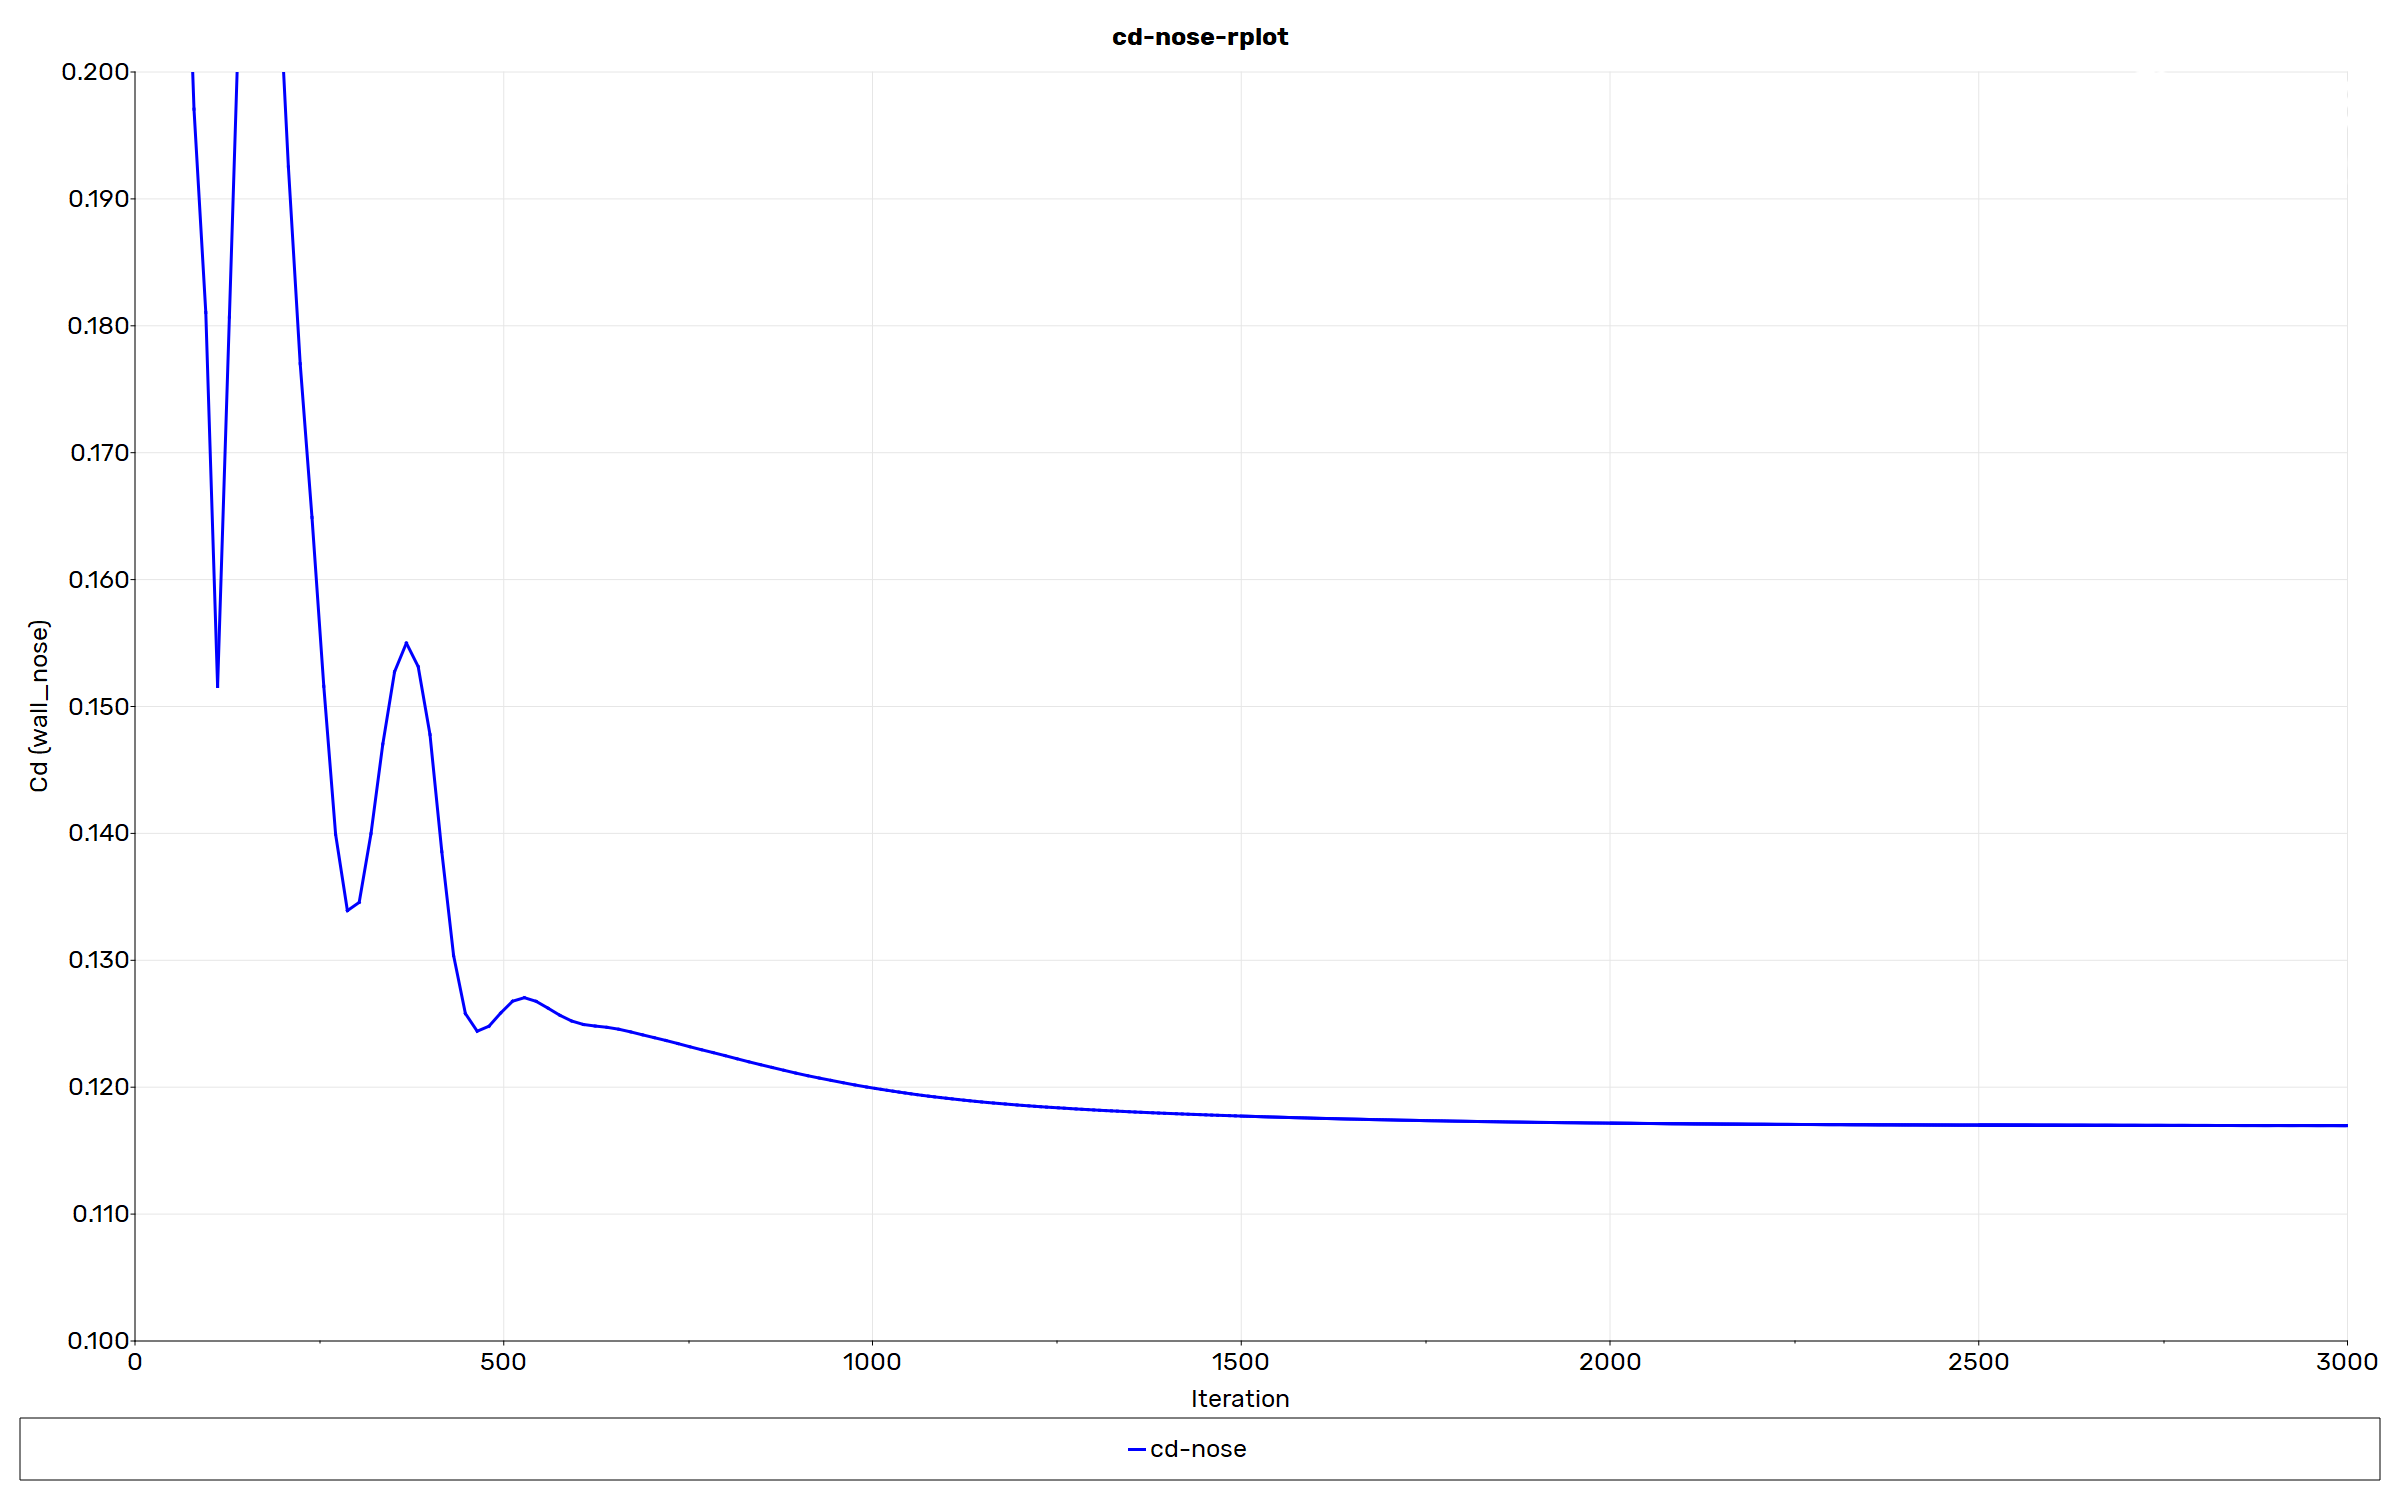
\includegraphics[width=\linewidth]{fluent_cd_M1.47}
\caption{$M = 1.47$, density-based.}
\end{subfigure}\hfill
\begin{subfigure}[t]{0.49\linewidth}
\centering
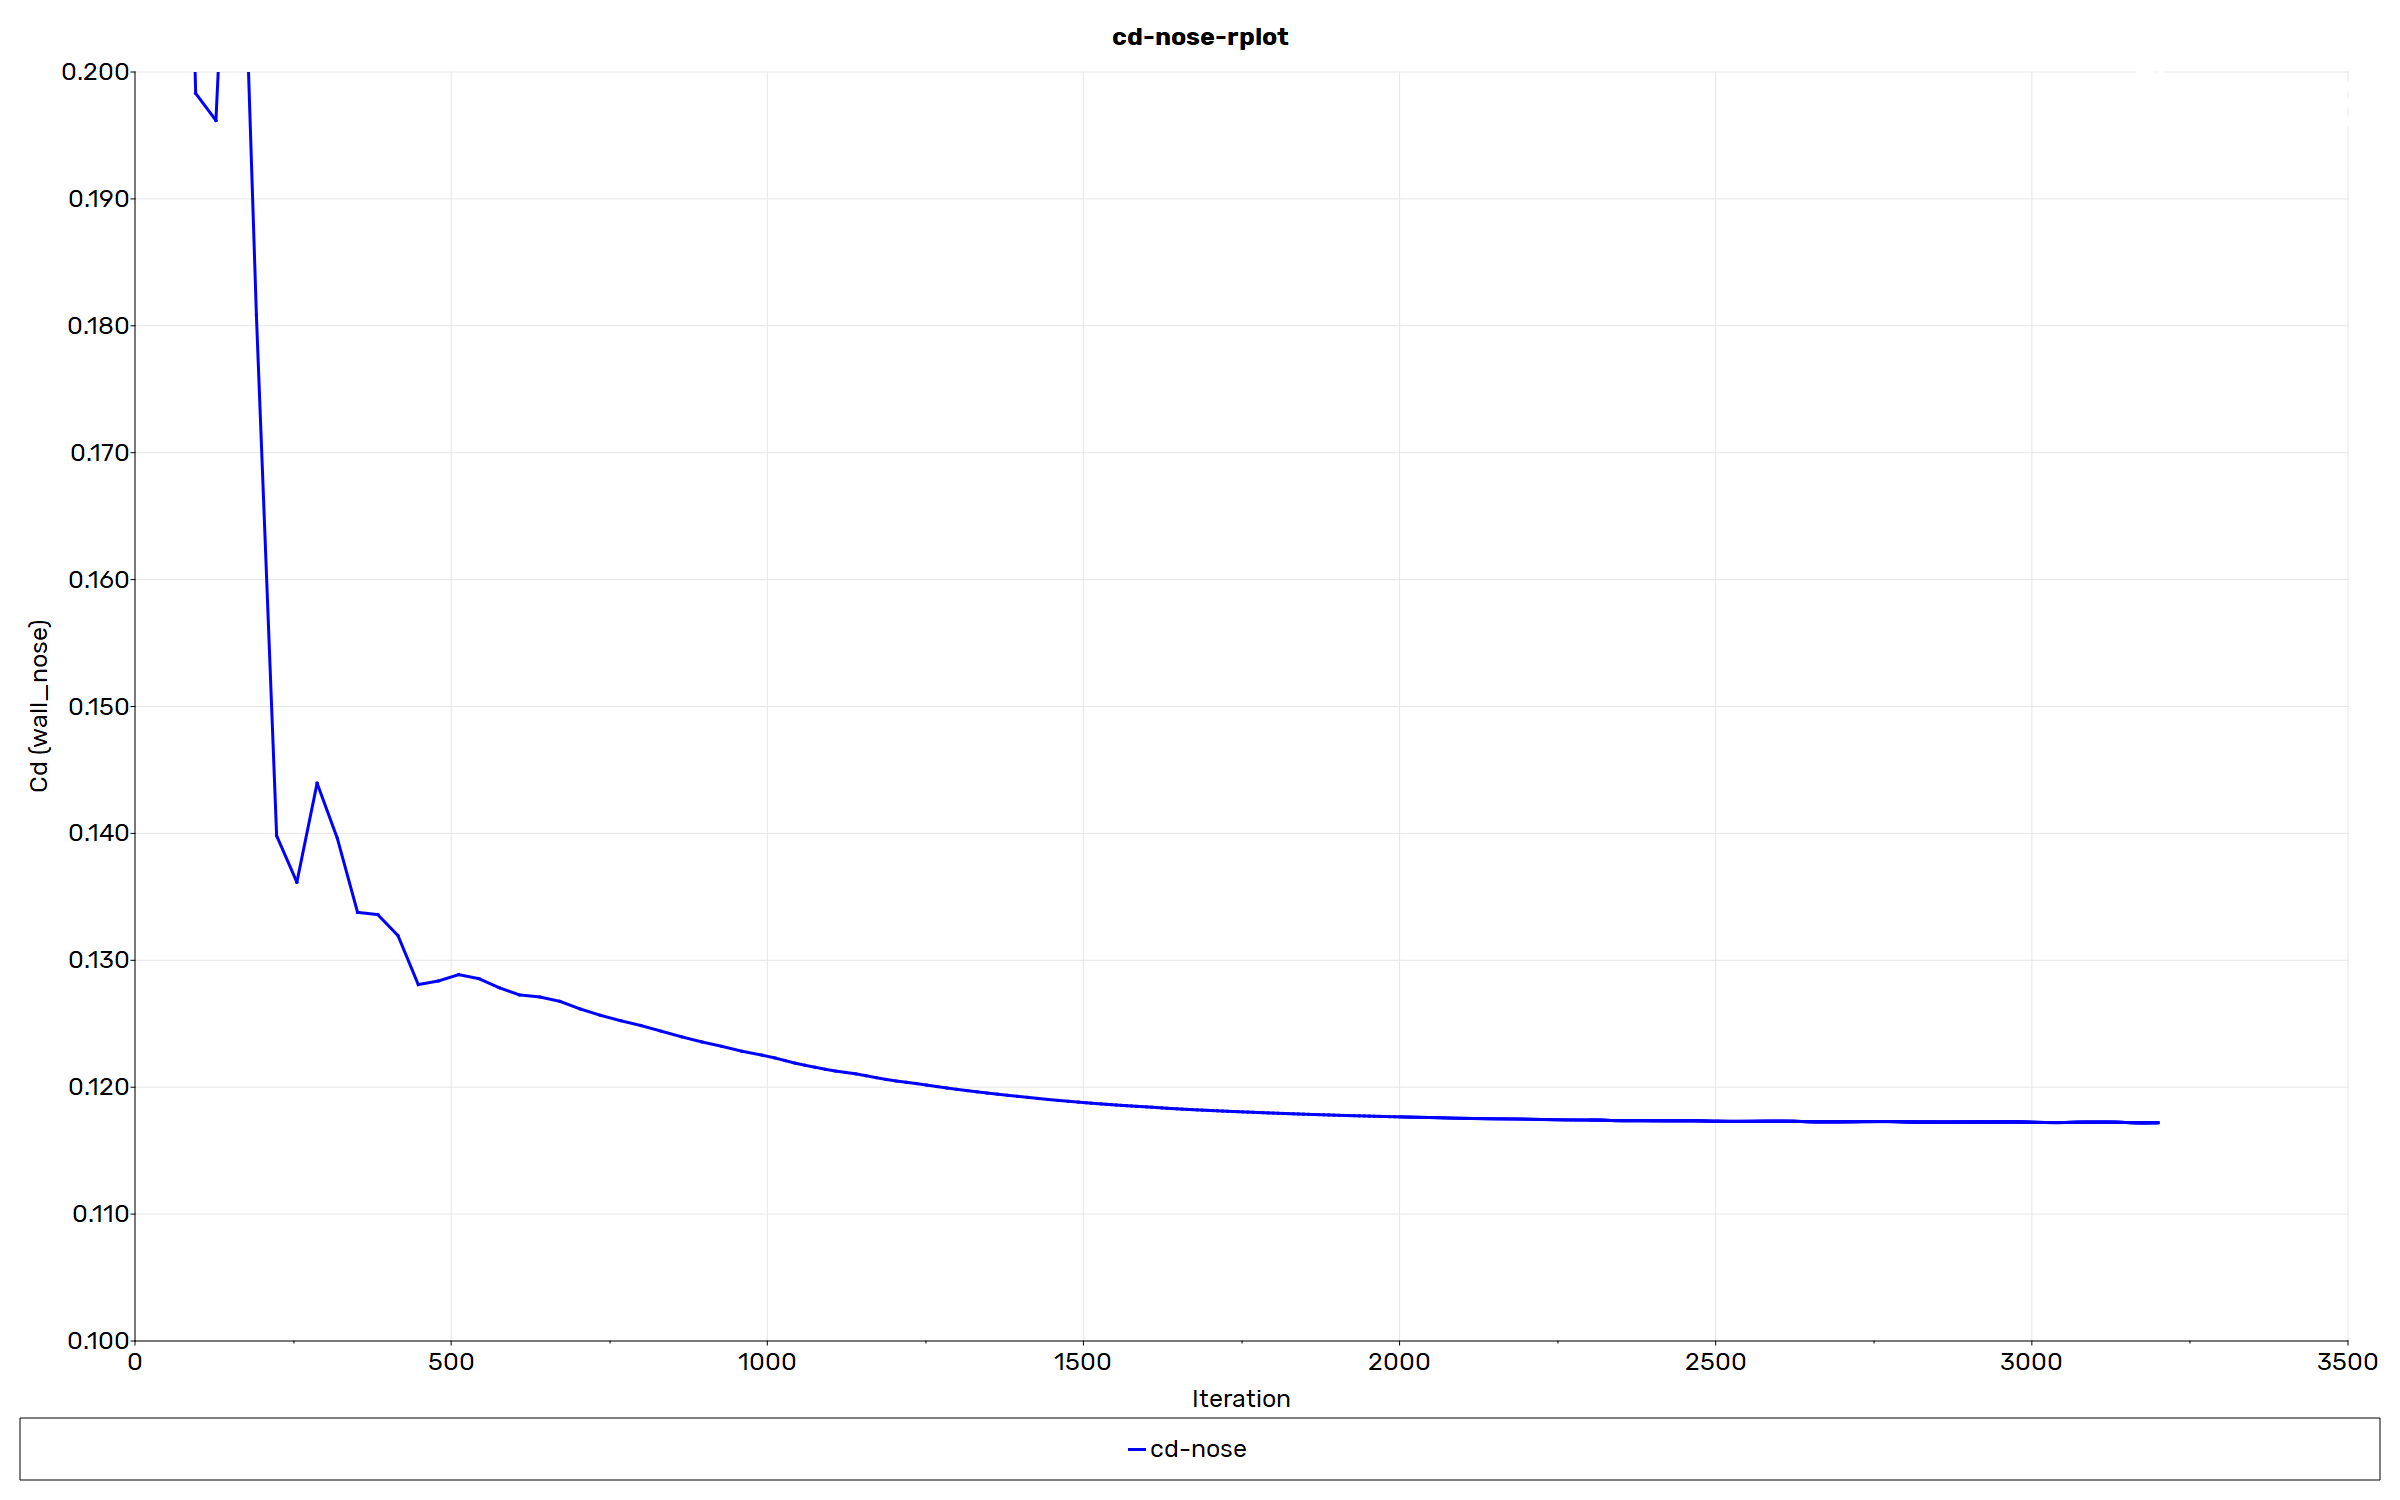
\includegraphics[width=\linewidth]{fluent_cd_M1.20}
\caption{$M = 1.2$, density-based.}
\end{subfigure}

\medskip
\begin{subfigure}[t]{0.49\linewidth}
\centering
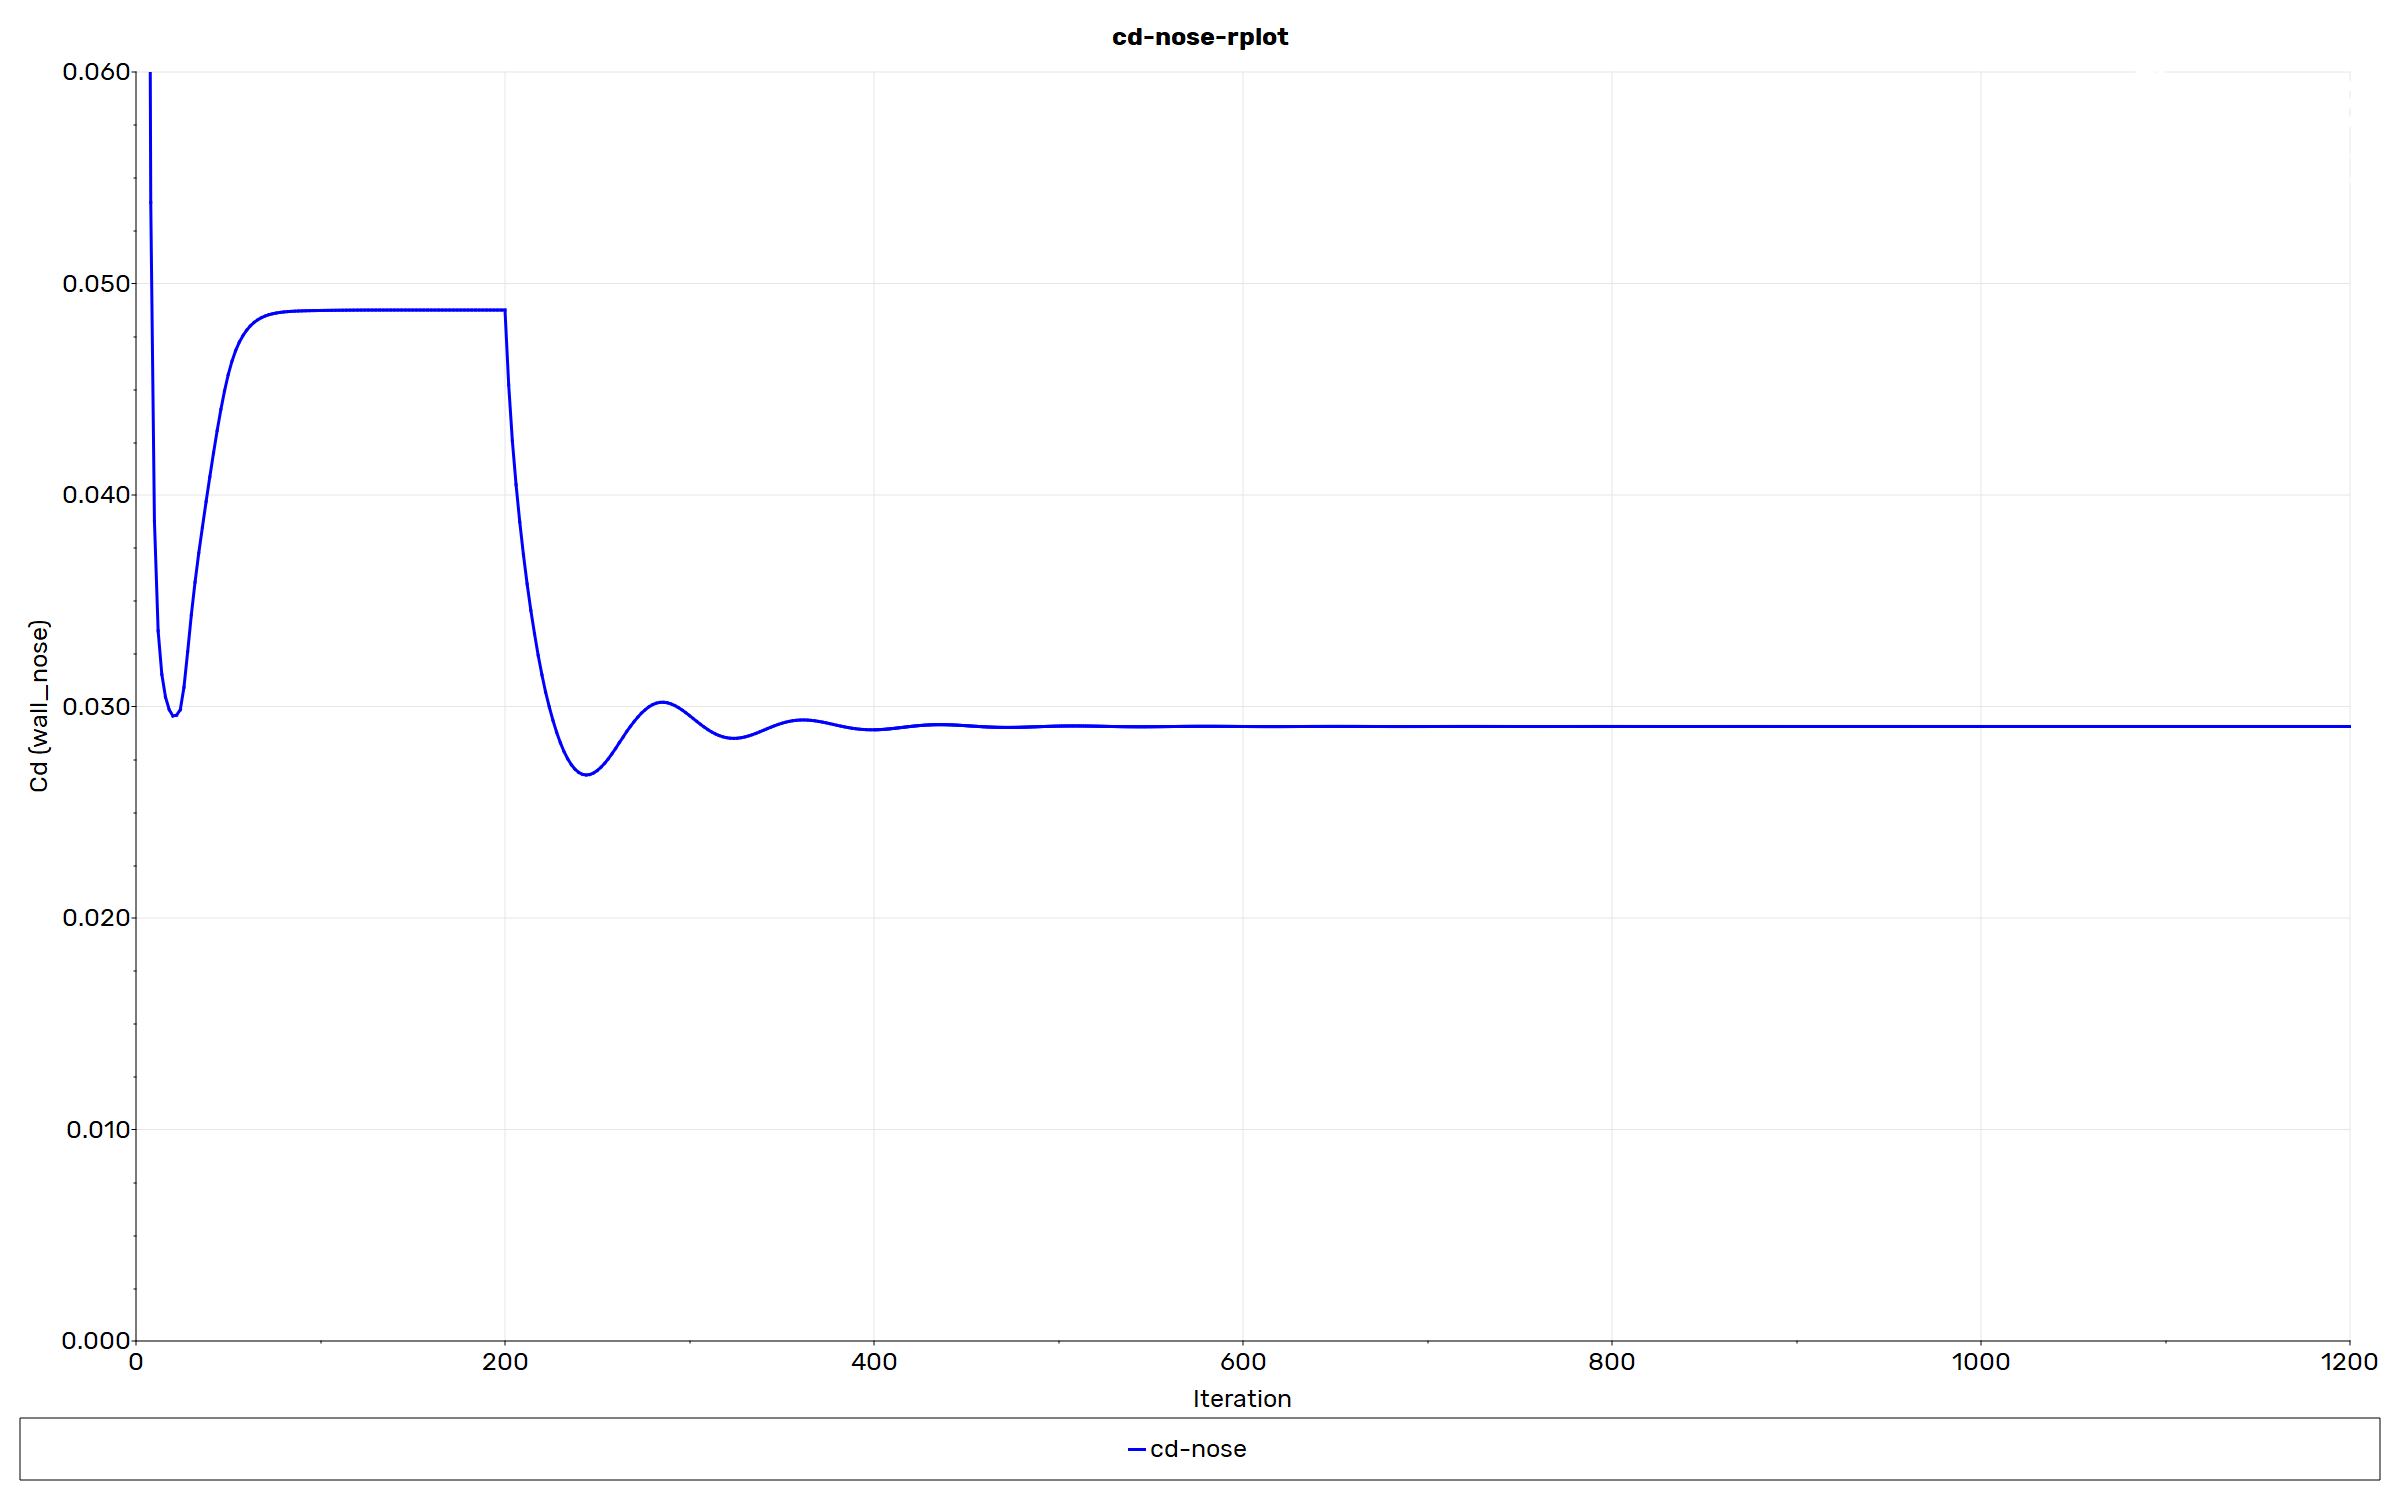
\includegraphics[width=\linewidth]{fluent_cd_M0.95}
\caption{$M = 0.95$, pressure-based.}
\end{subfigure}
\caption{The \texttt{cd-nose} monitor of the three converged runs (Fluent report plots). The vertical
axis is fixed (0.10--0.20 above $M = 1$, 0--0.06 at $M = 0.95$), so the first iterations go off the top.
Second order starts at iteration 400 in (a) and (b) and at iteration 200 in (c).}
\label{fig:history}
\end{figure}

Each curve shows a first-order transient, a drop at the switch to second order (first order adds numerical
dissipation, seen as extra drag), then a slow decay; the last per cent takes 1500--2000 iterations.
First-order values, such as 0.0488 at $M = 0.95$, are only starting fields.

\begin{figure}[H]
\centering
\begin{subfigure}[t]{0.49\linewidth}
\centering
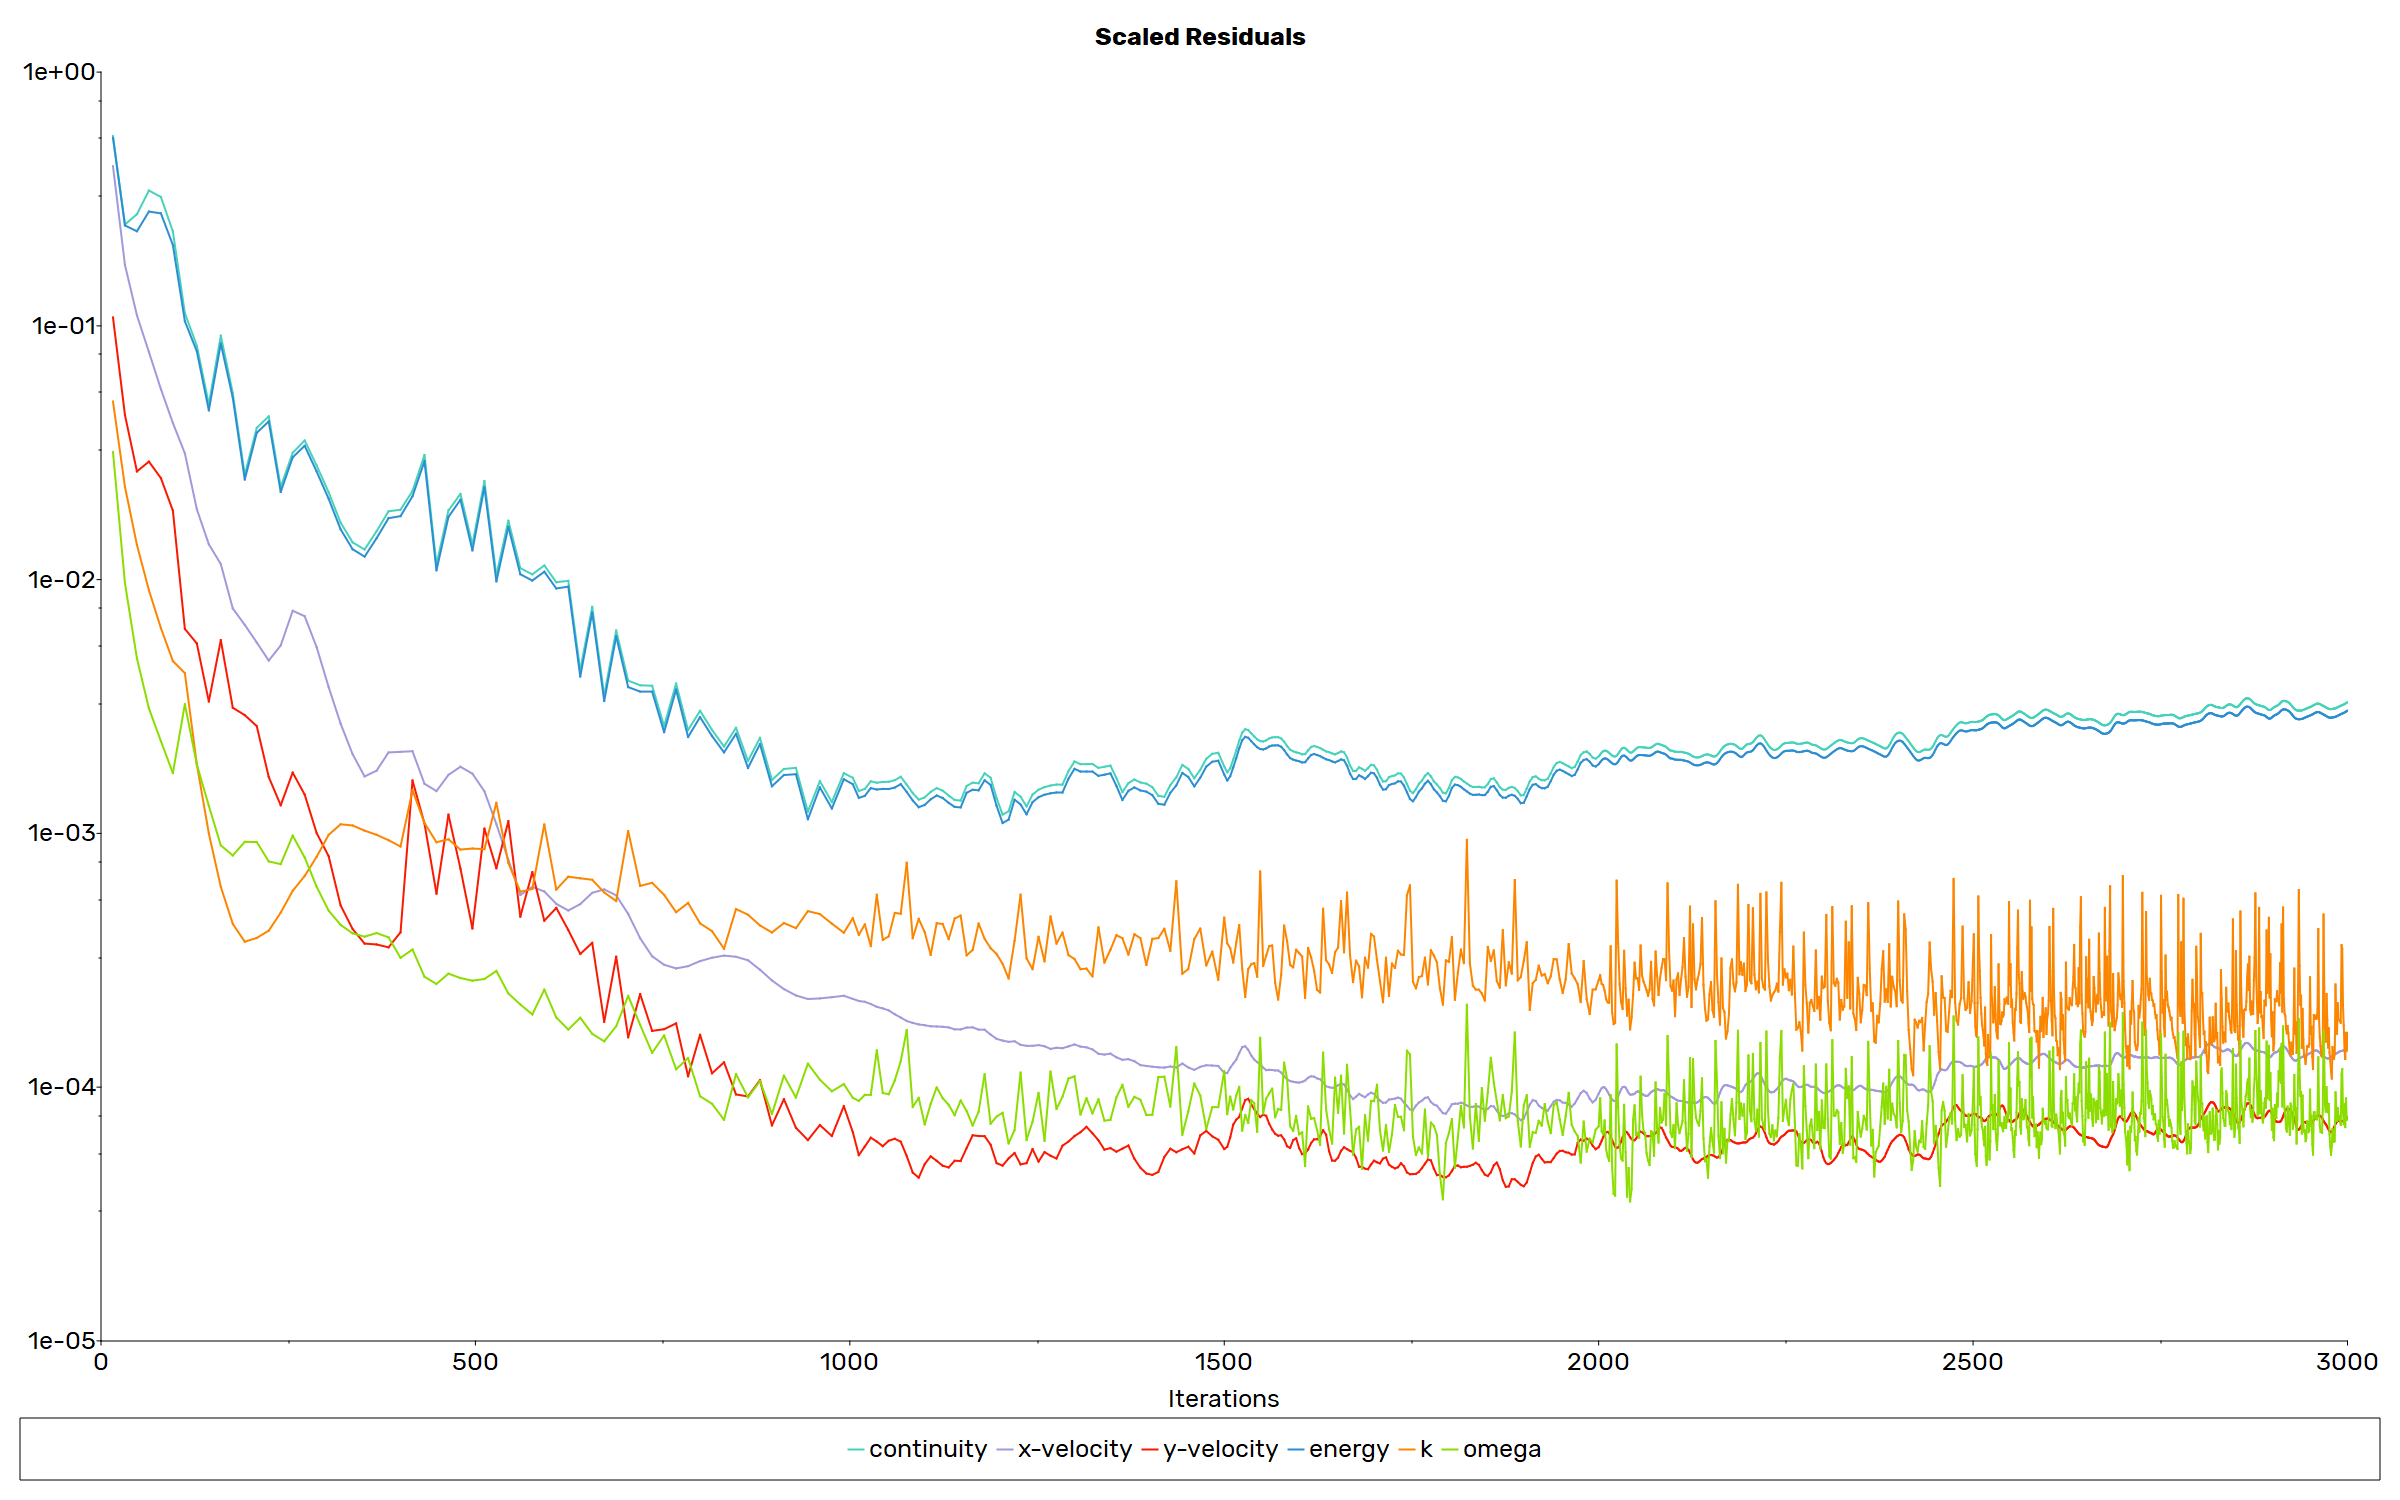
\includegraphics[width=\linewidth]{fluent_residuals_M1.47}
\caption{$M = 1.47$, density-based.}
\end{subfigure}\hfill
\begin{subfigure}[t]{0.49\linewidth}
\centering
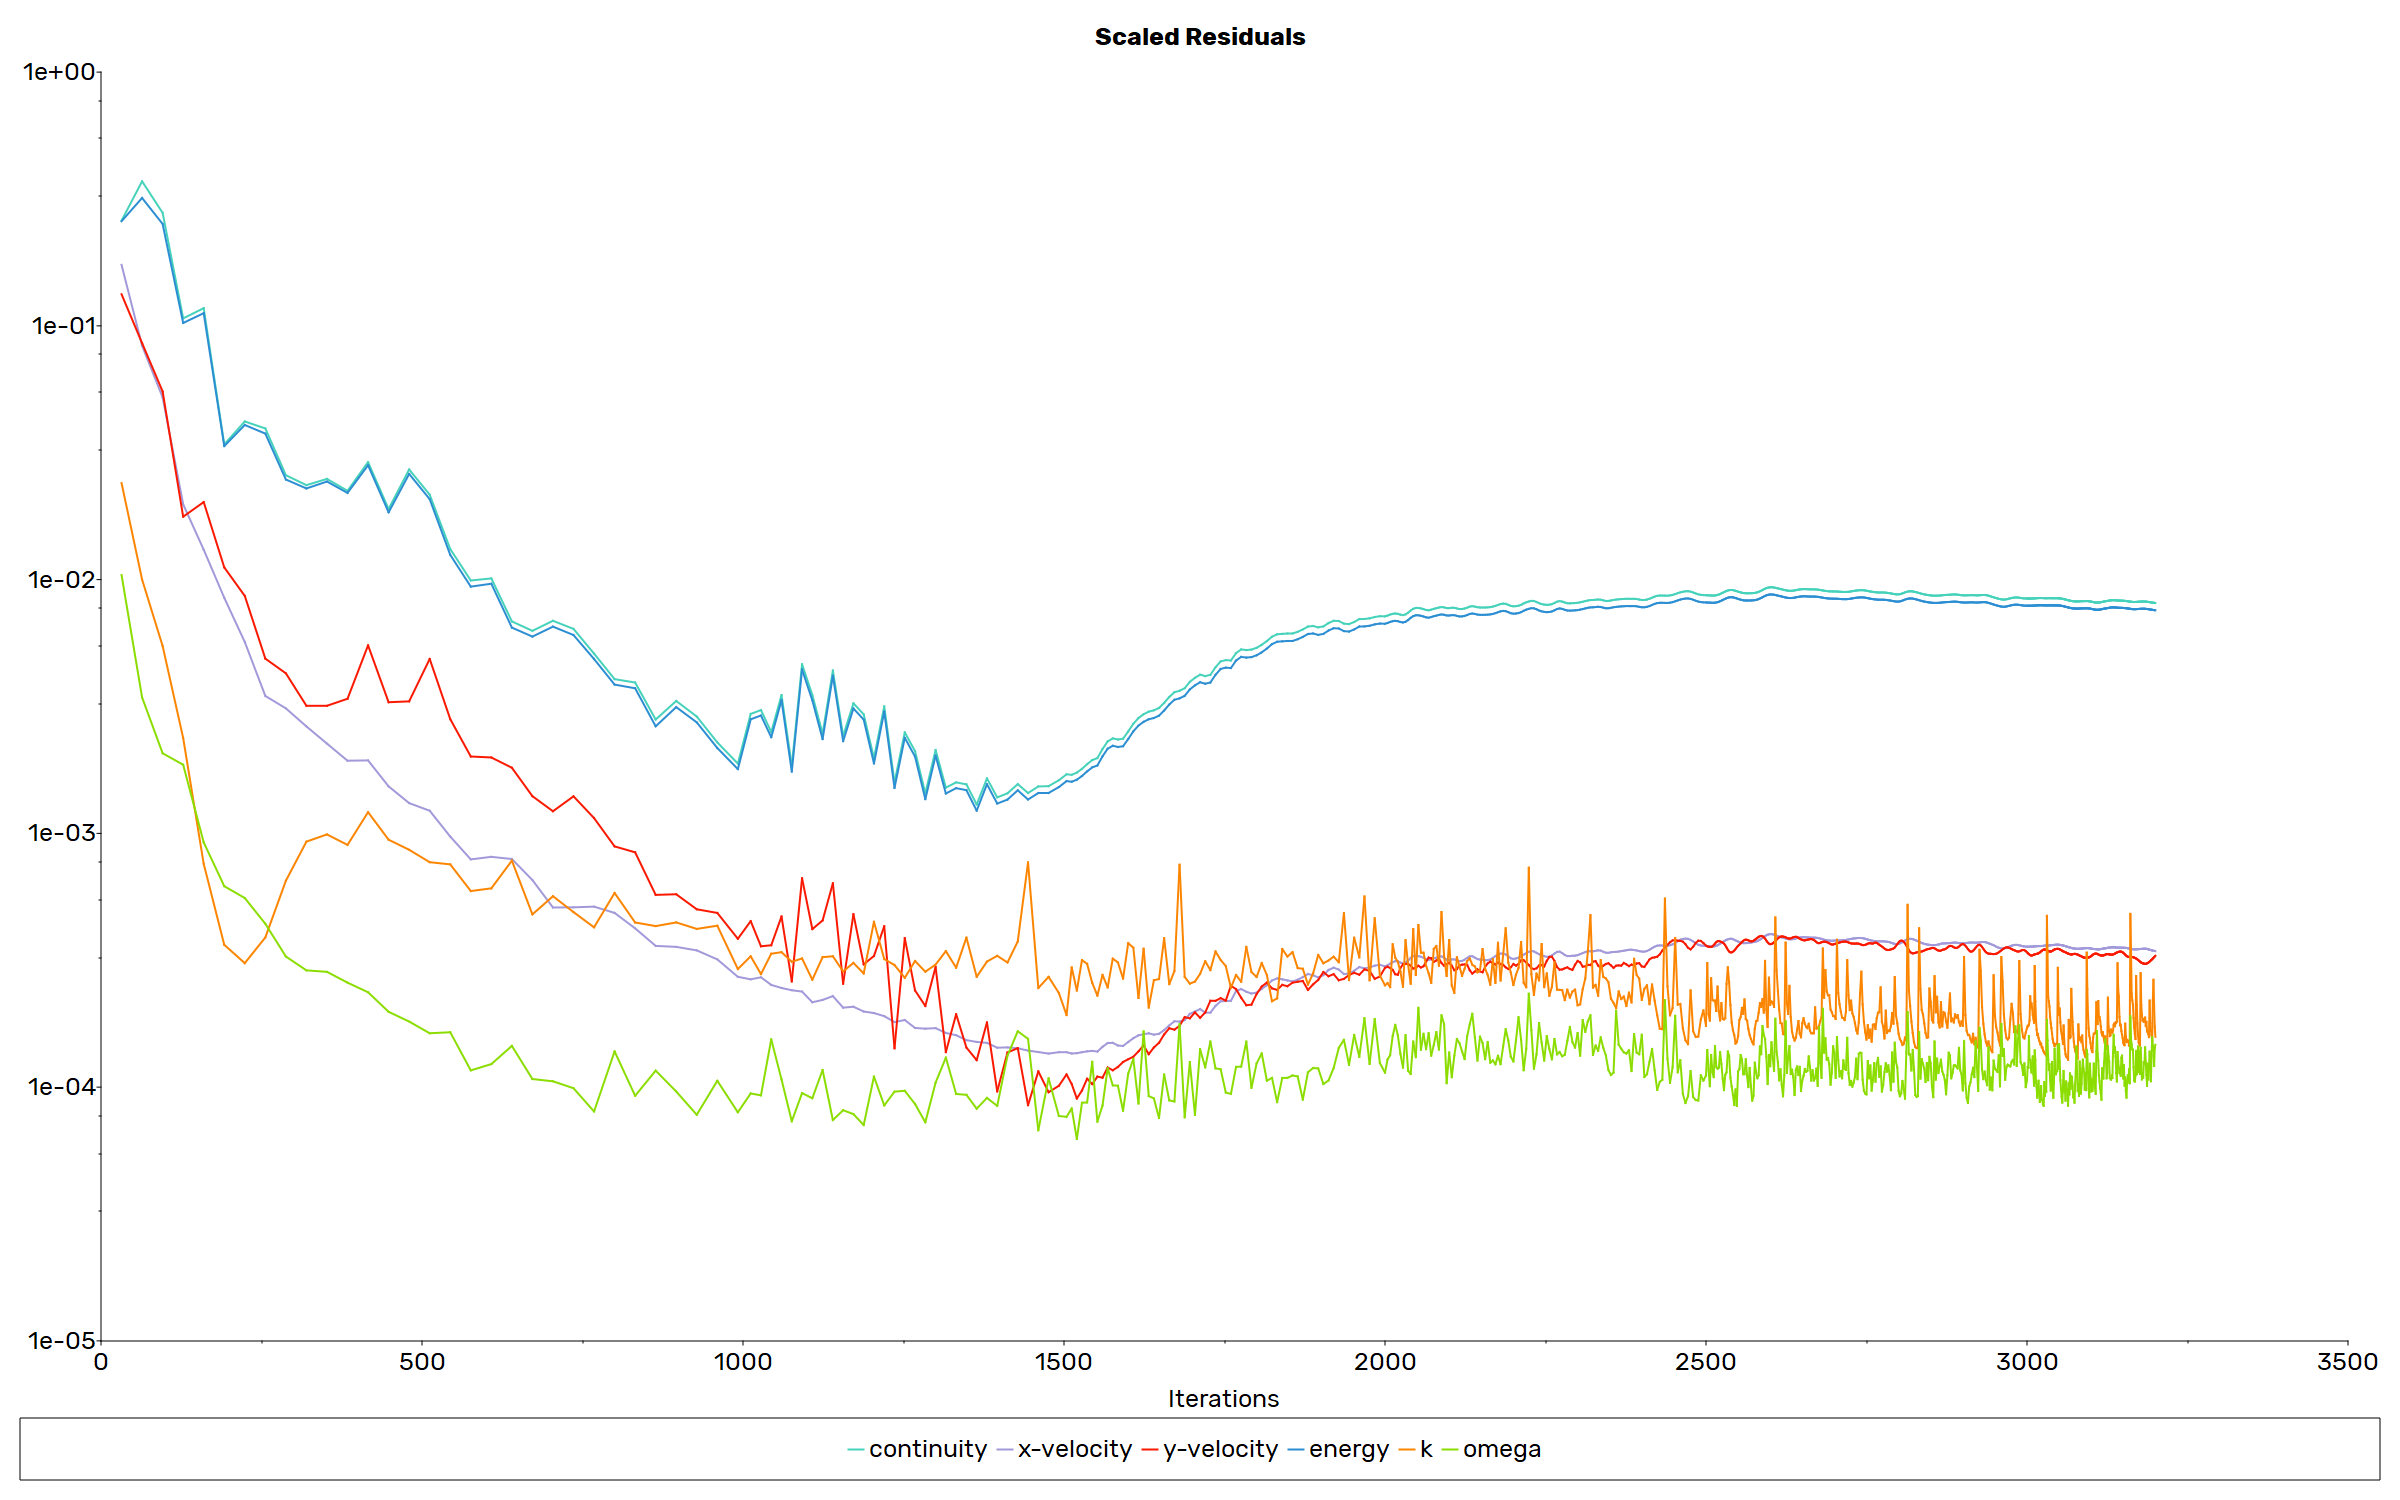
\includegraphics[width=\linewidth]{fluent_residuals_M1.20}
\caption{$M = 1.2$, density-based.}
\end{subfigure}

\medskip
\begin{subfigure}[t]{0.49\linewidth}
\centering
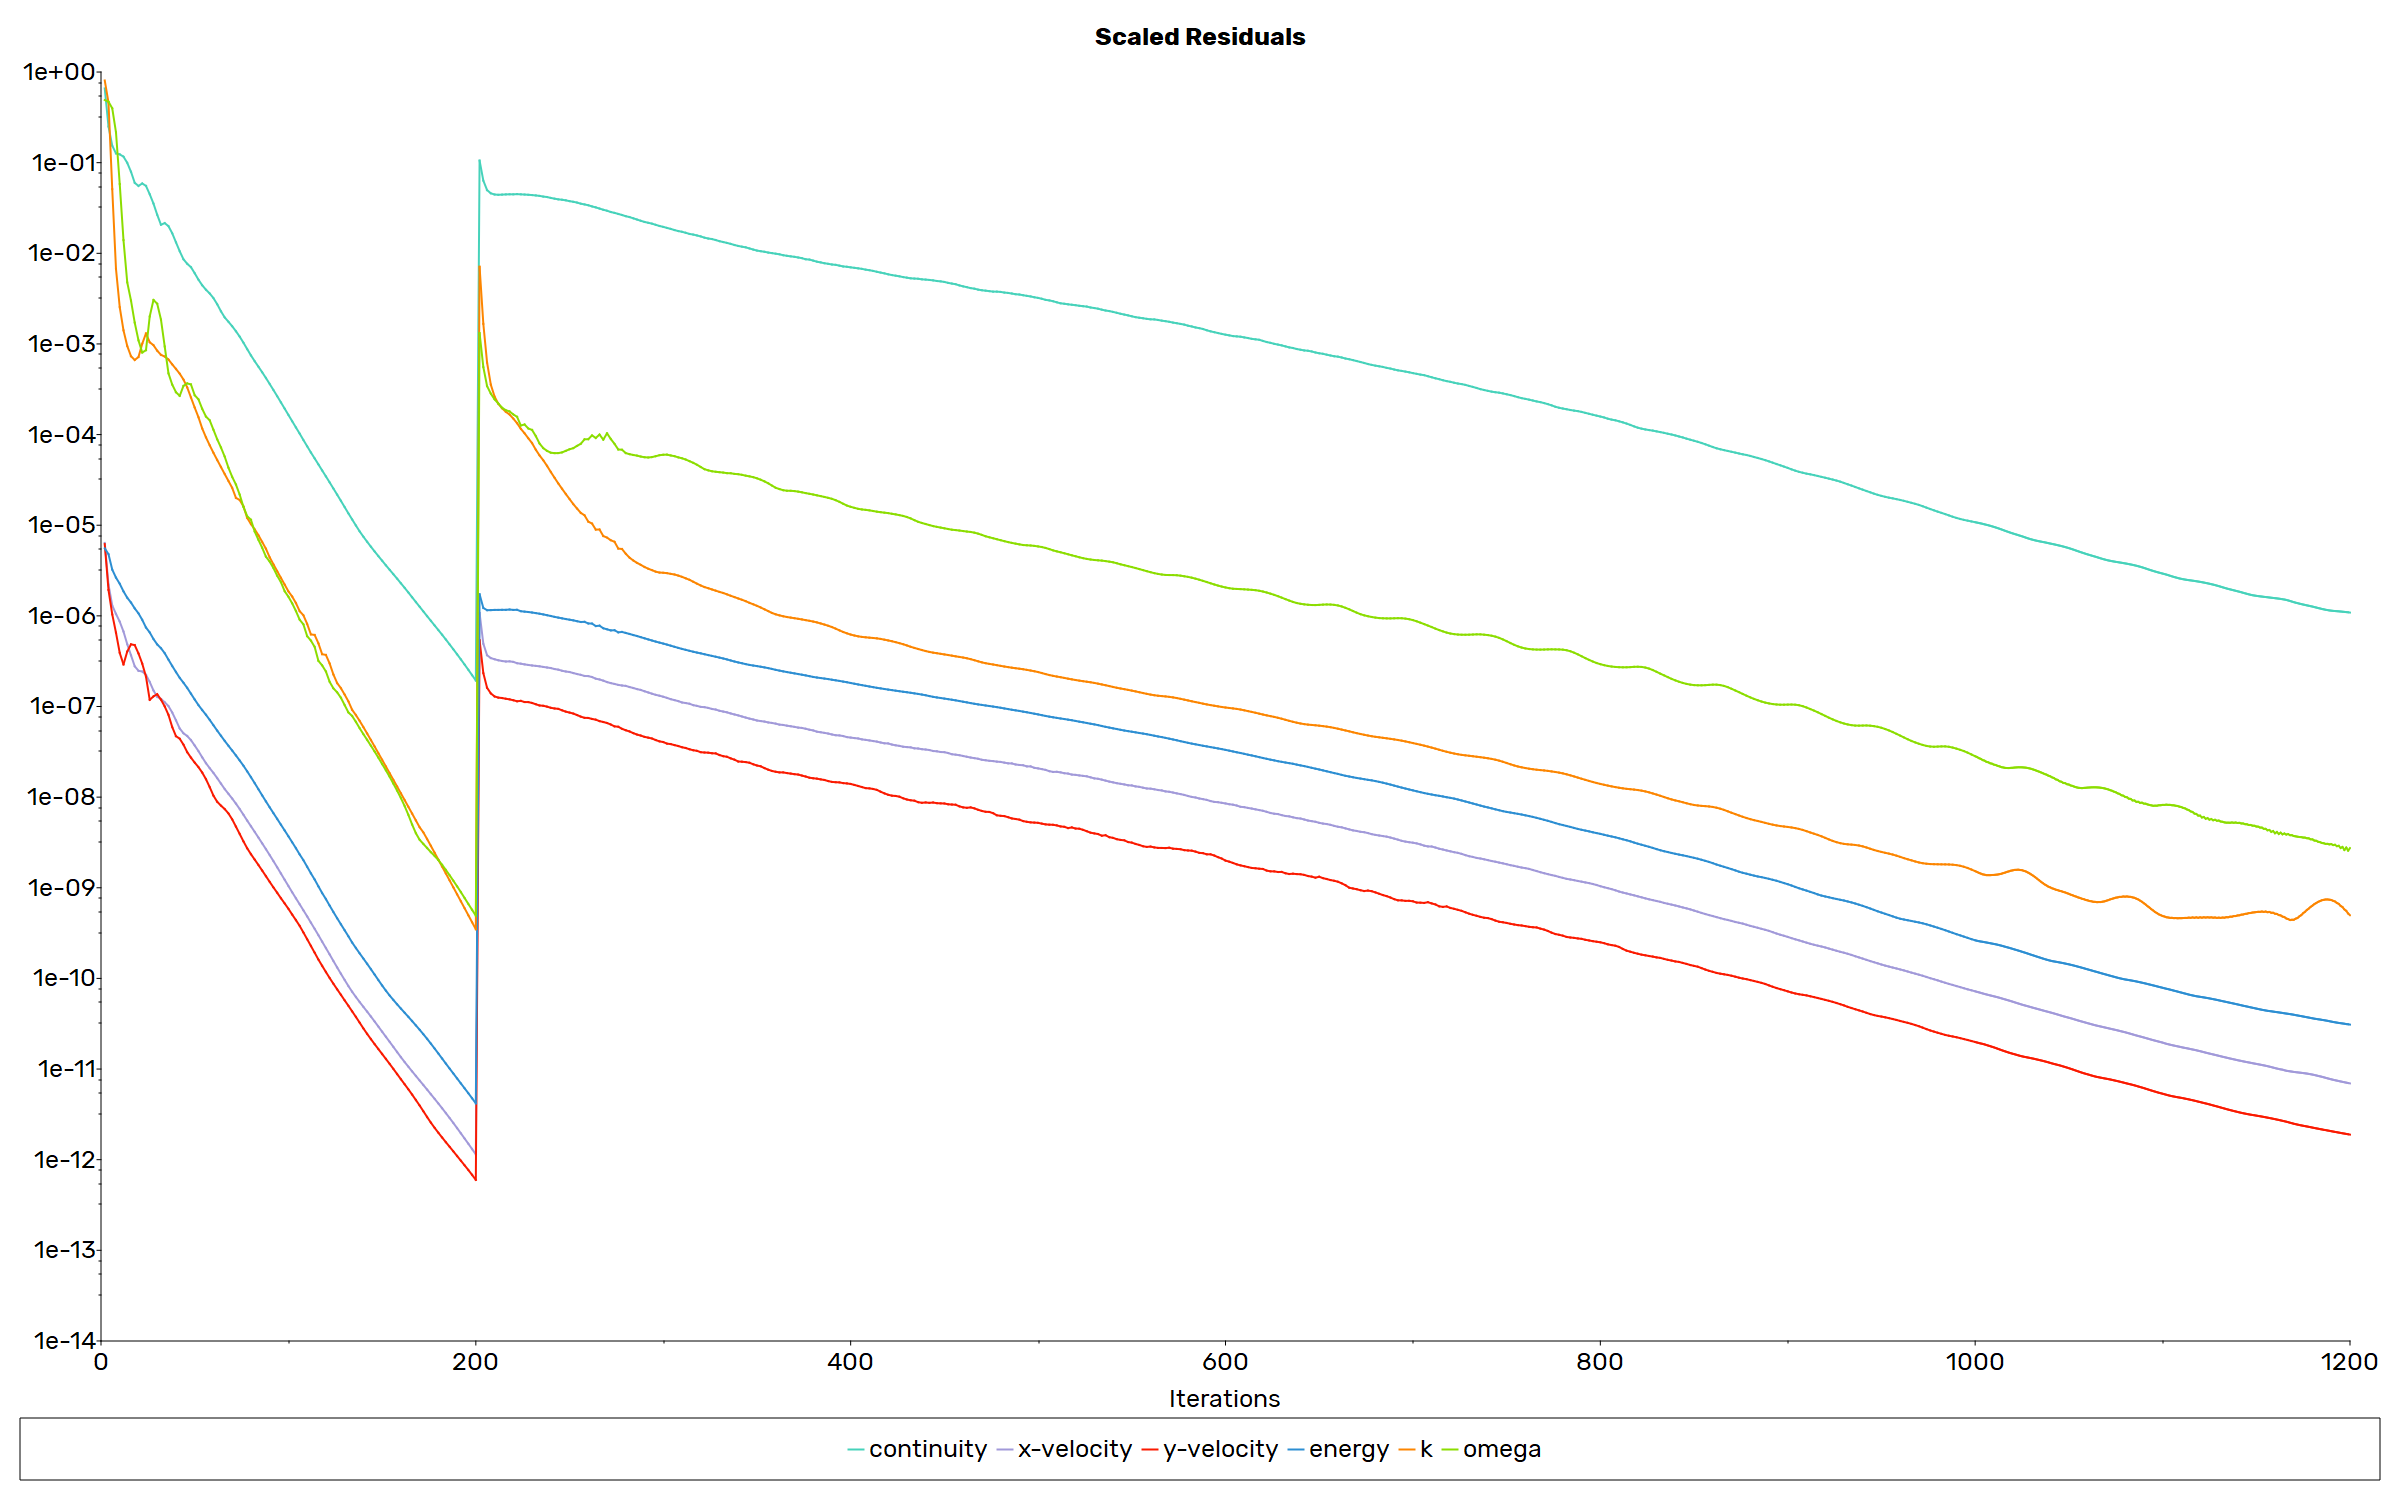
\includegraphics[width=\linewidth]{fluent_residuals_M0.95}
\caption{$M = 0.95$, pressure-based.}
\end{subfigure}
\caption{Scaled residuals from Fluent. At $M = 1.47$ they level off at $10^{-4}$--$3\cdot10^{-3}$
while $C_D$ is already constant (Figure~\ref{fig:history}a), which is why convergence is judged on
$C_D$.}
\label{fig:residuals}
\end{figure}

\section{Results of study A}
\label{sec:results}

\subsection{Drag of the nose}

\begin{figure}[H]
\centering
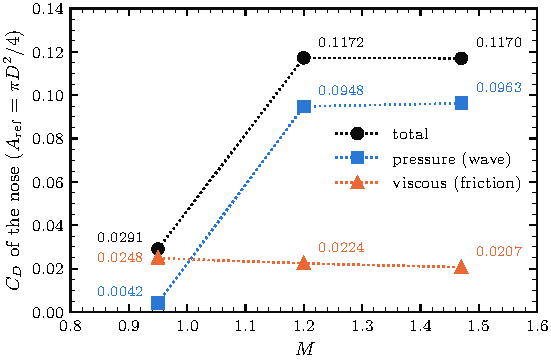
\includegraphics[width=0.62\linewidth]{fig_cd_mach}
\caption{Drag coefficient of the nose (\zone{wall\_nose}) against Mach: pressure (wave), viscous and total.
Drawn from the Fluent force reports of the three runs (Fluent cannot plot across separate runs); the
dotted lines only join the three runs.}
\label{fig:cdmach}
\end{figure}

\begin{itemize}
\item \textbf{Supersonic.} The pressure part is 0.095--0.096, 81--82\,\% of the total, and nearly
constant between $M = 1.2$ and 1.47.
\item \textbf{Transonic.} The pressure part is only 0.0042: the overpressure at the tip is almost
cancelled by the suction on the rear of the nose. Friction is 85\,\% of the total.
\item \textbf{Friction} falls from 0.0248 to 0.0207 as $\mathrm{Re}_x$ rises and the wall gets hotter.
\end{itemize}

\subsection{Flow field}

\begin{figure}[H]
\centering
\begin{subfigure}[t]{0.32\linewidth}
\centering
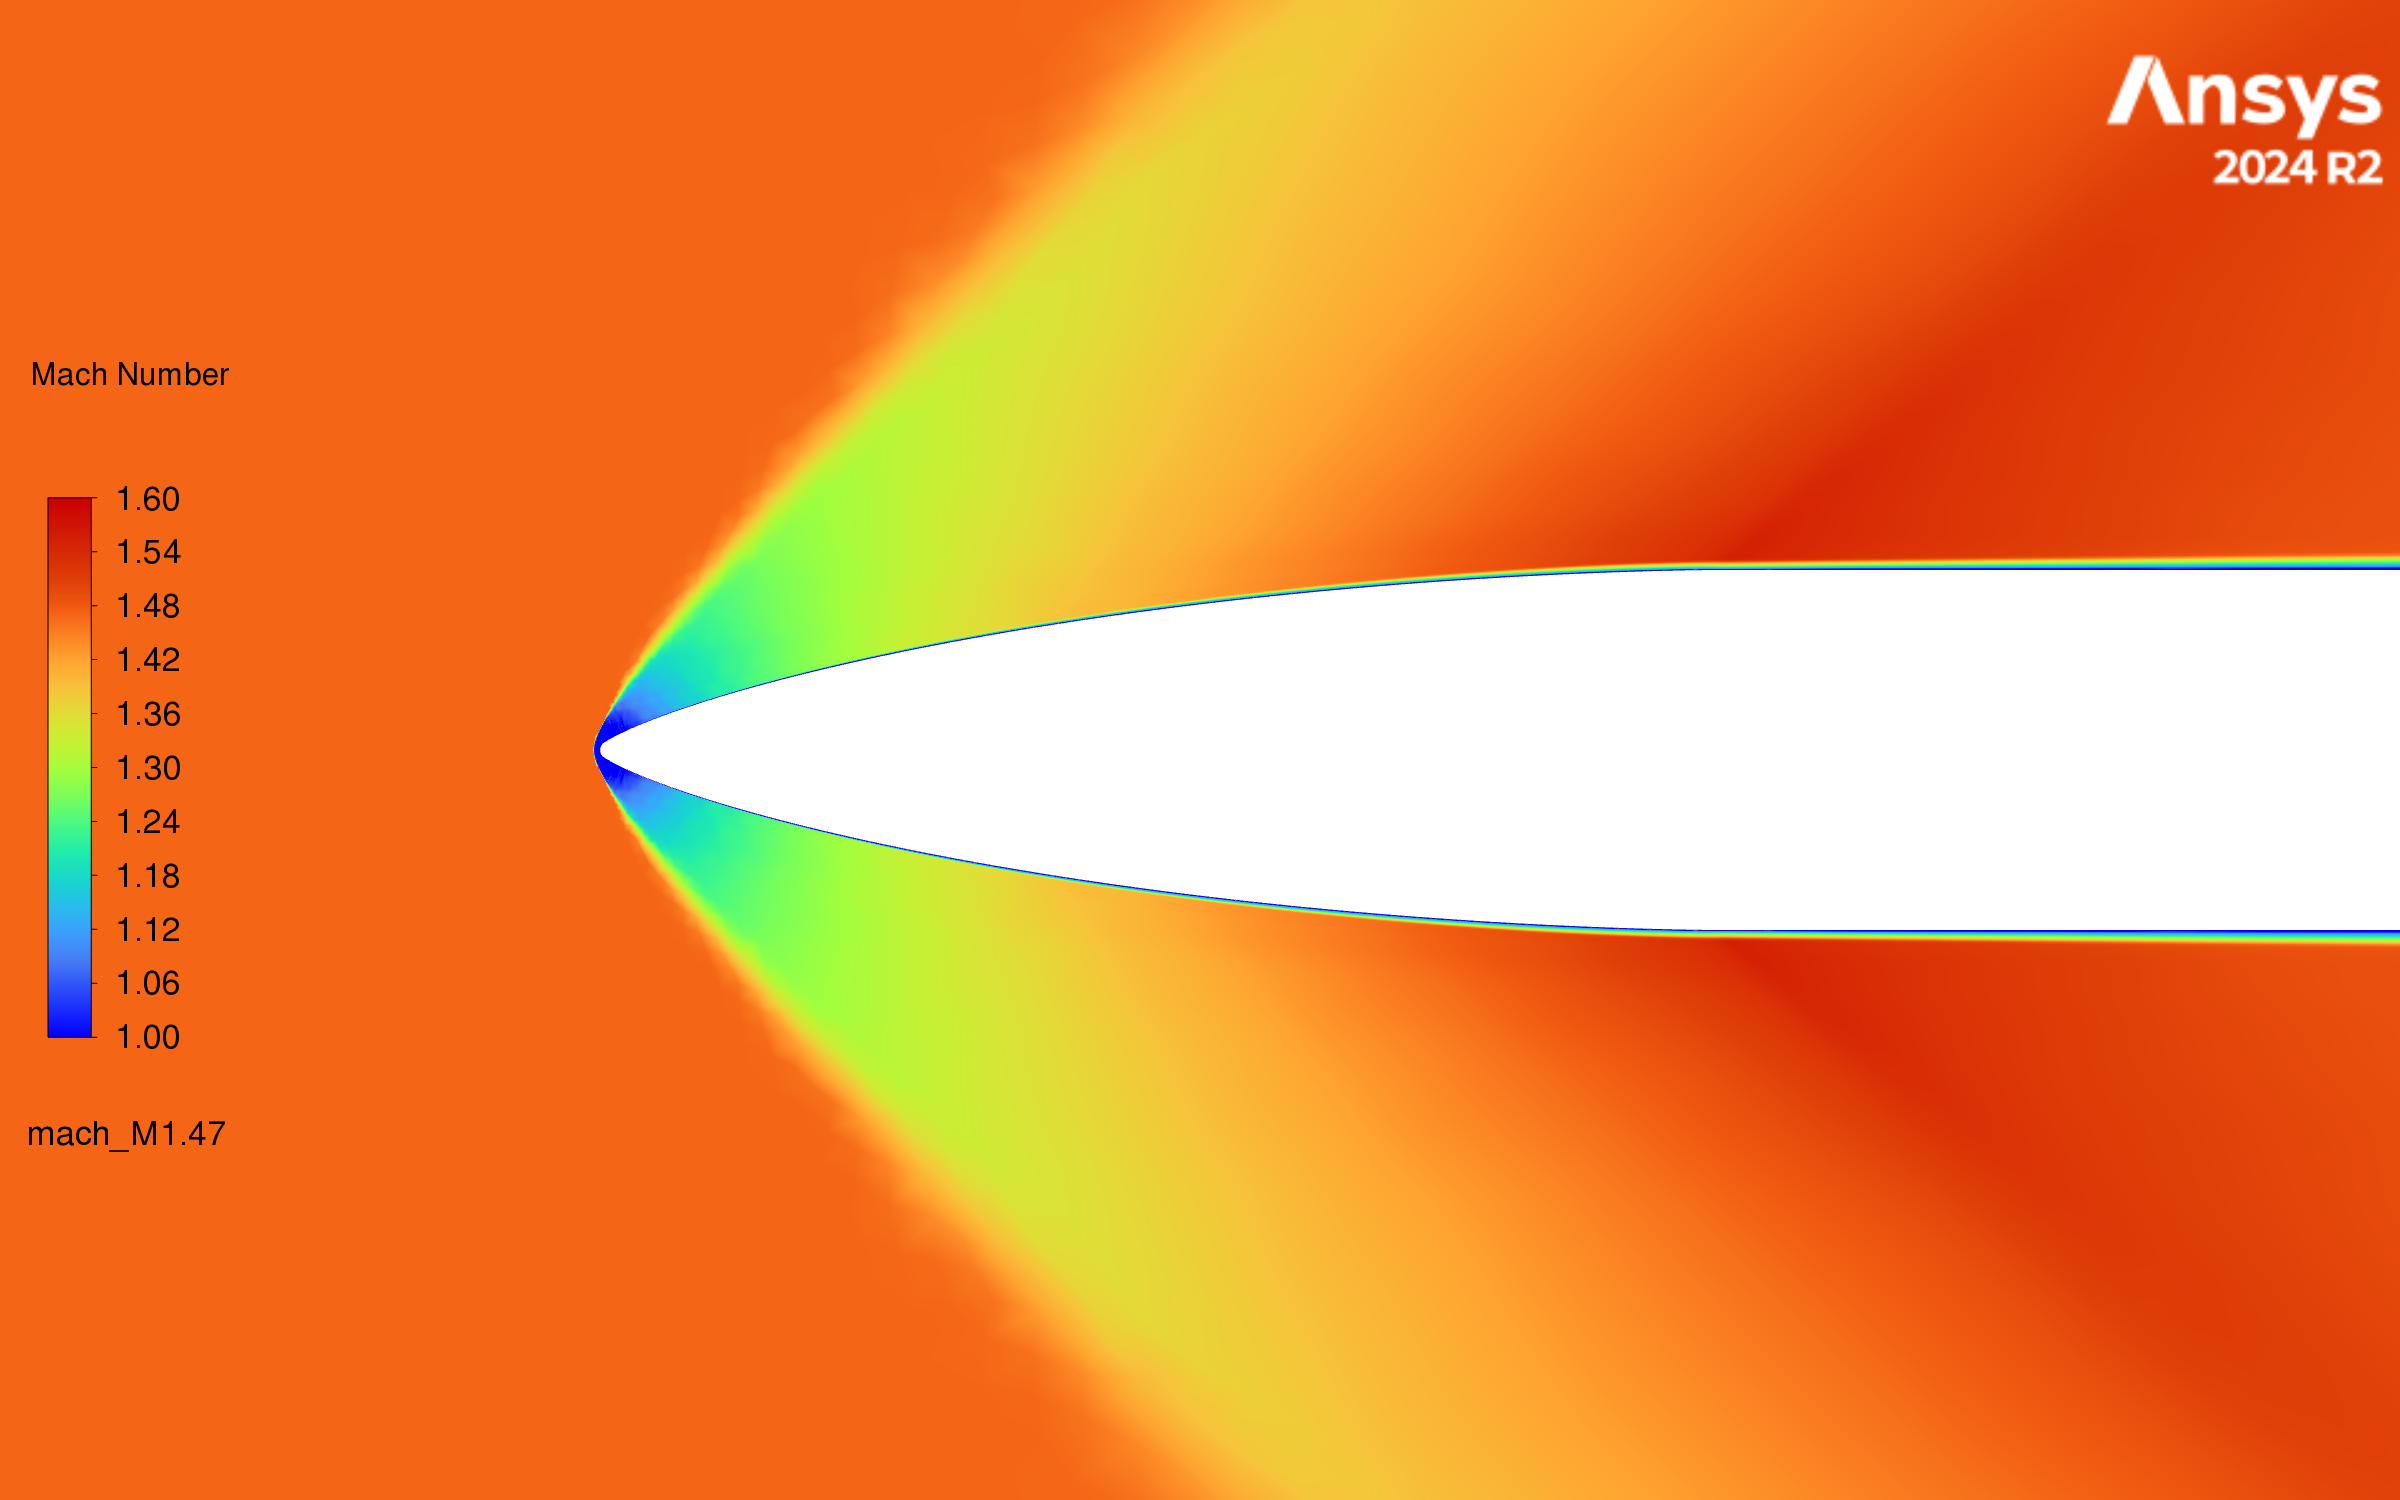
\includegraphics[width=\linewidth]{fluent_mach_M1.47}
\caption{$M = 1.47$ (1.0--1.6).}
\end{subfigure}\hfill
\begin{subfigure}[t]{0.32\linewidth}
\centering
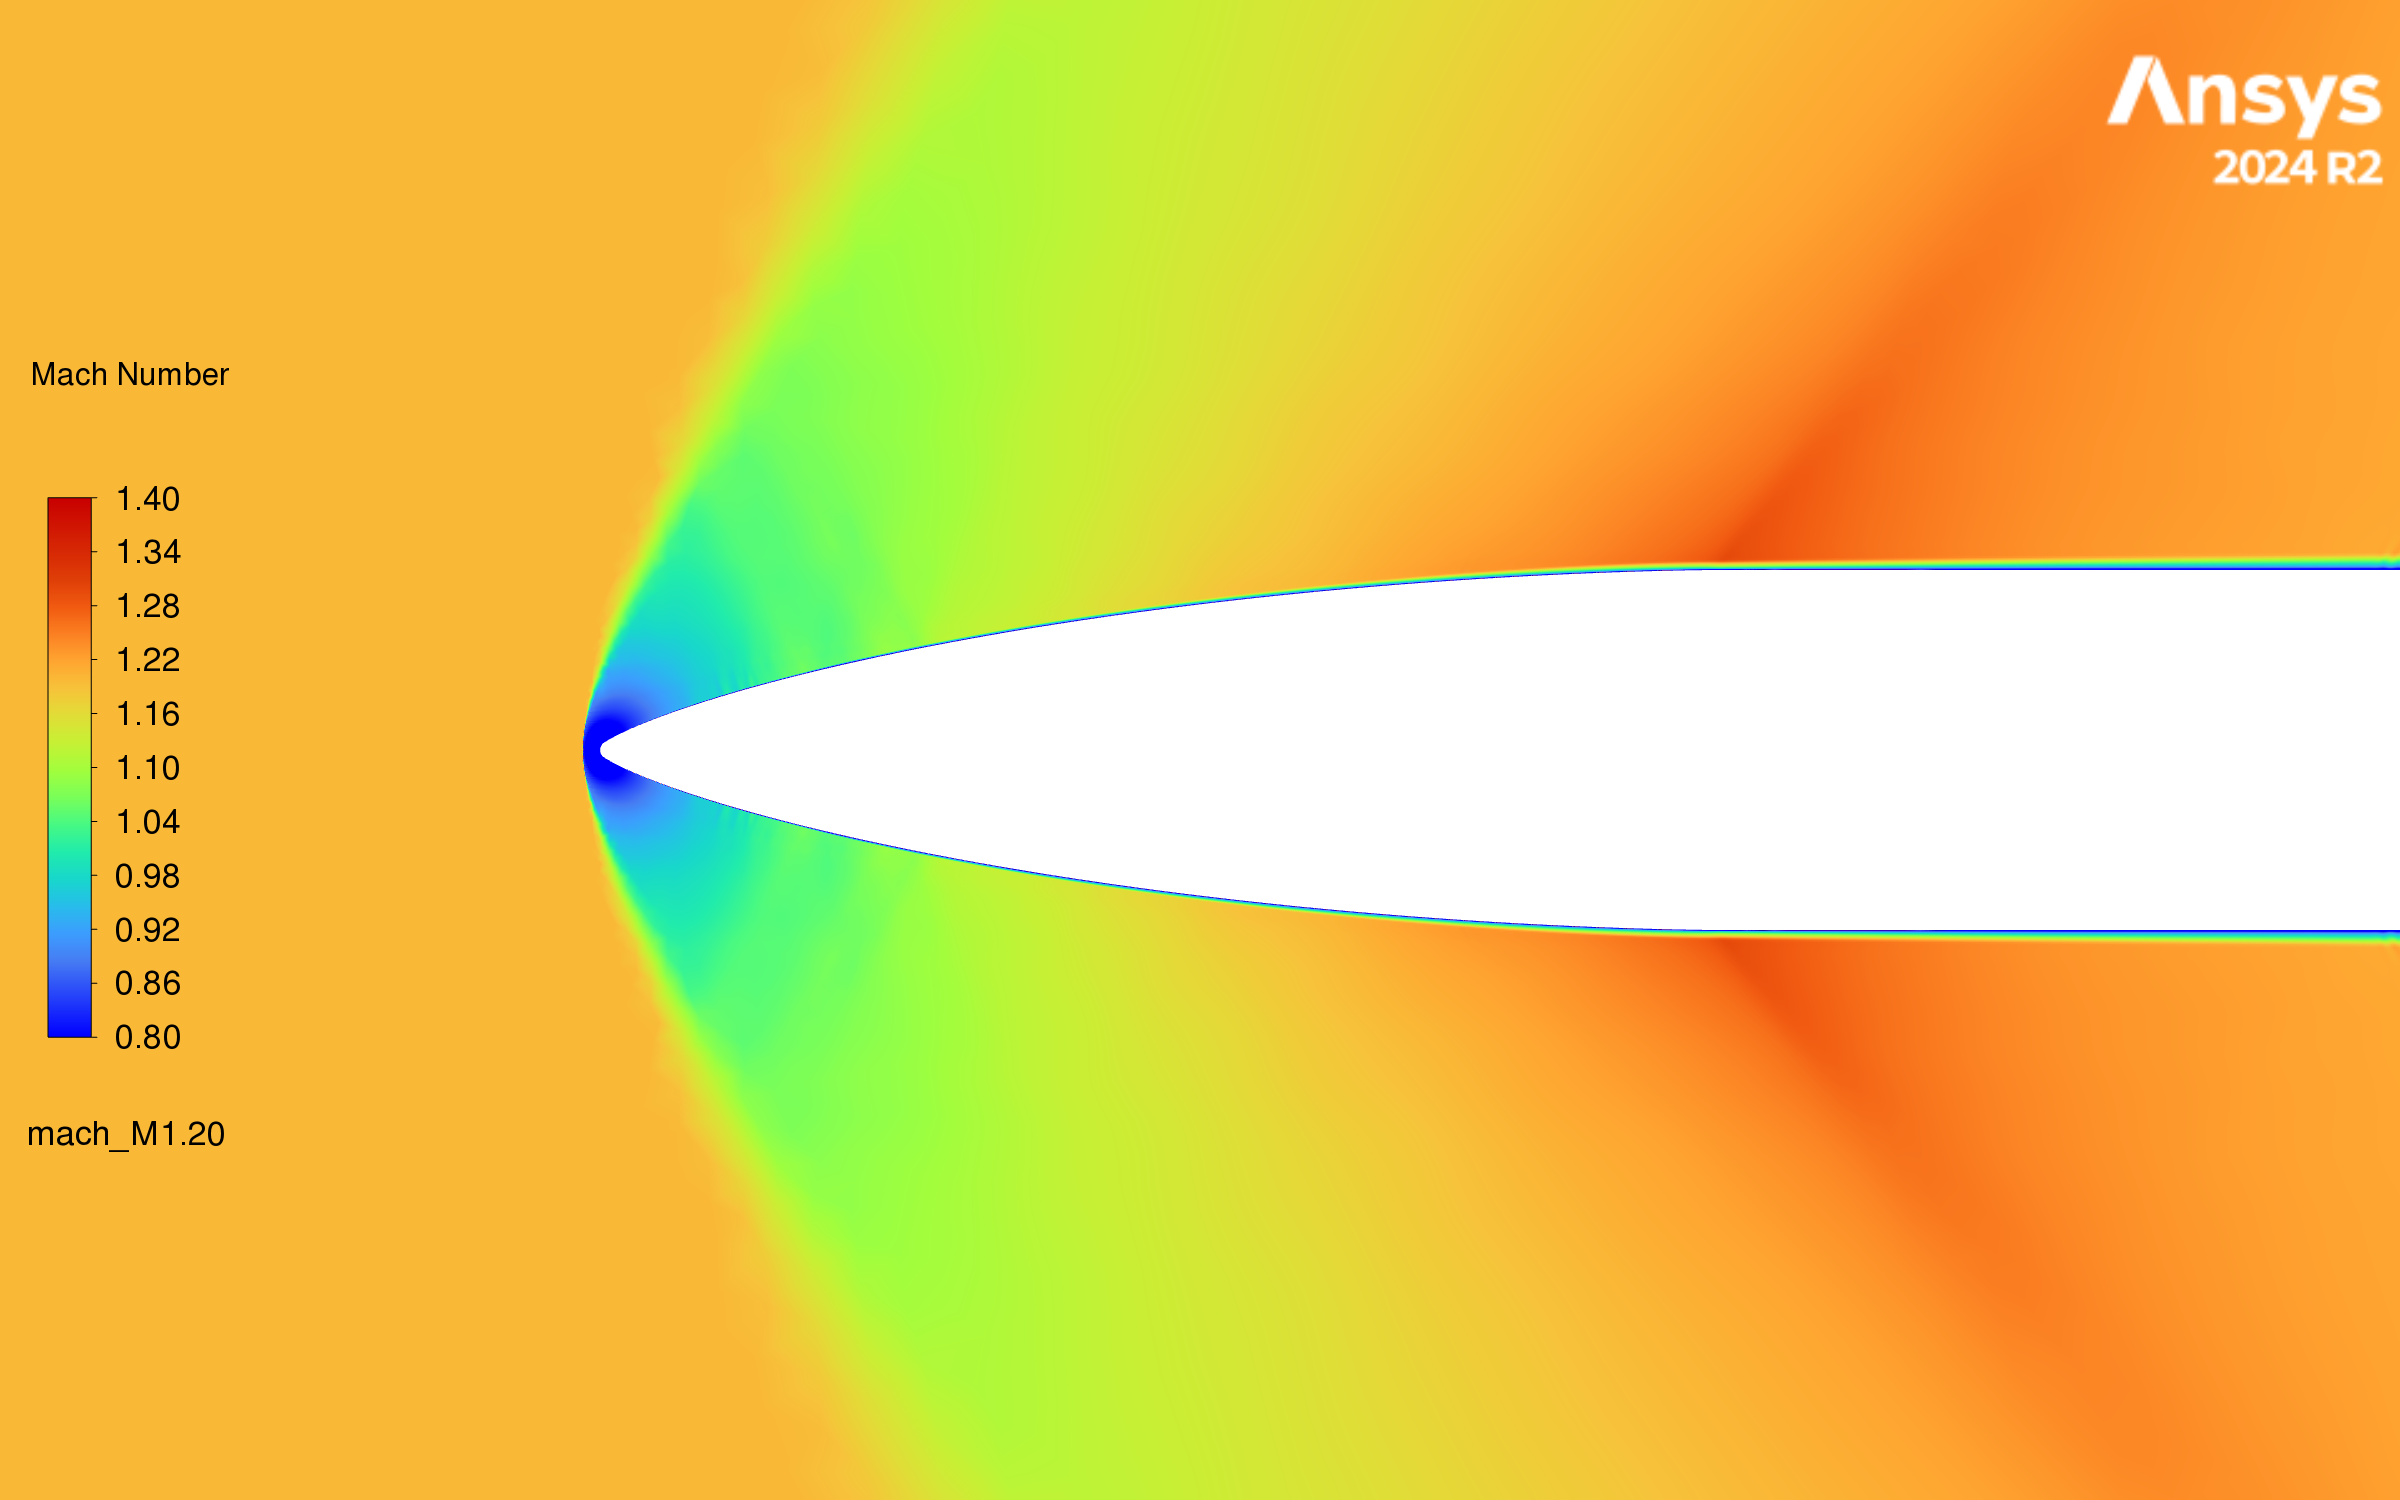
\includegraphics[width=\linewidth]{fluent_mach_M1.20}
\caption{$M = 1.2$ (0.8--1.4).}
\end{subfigure}\hfill
\begin{subfigure}[t]{0.32\linewidth}
\centering
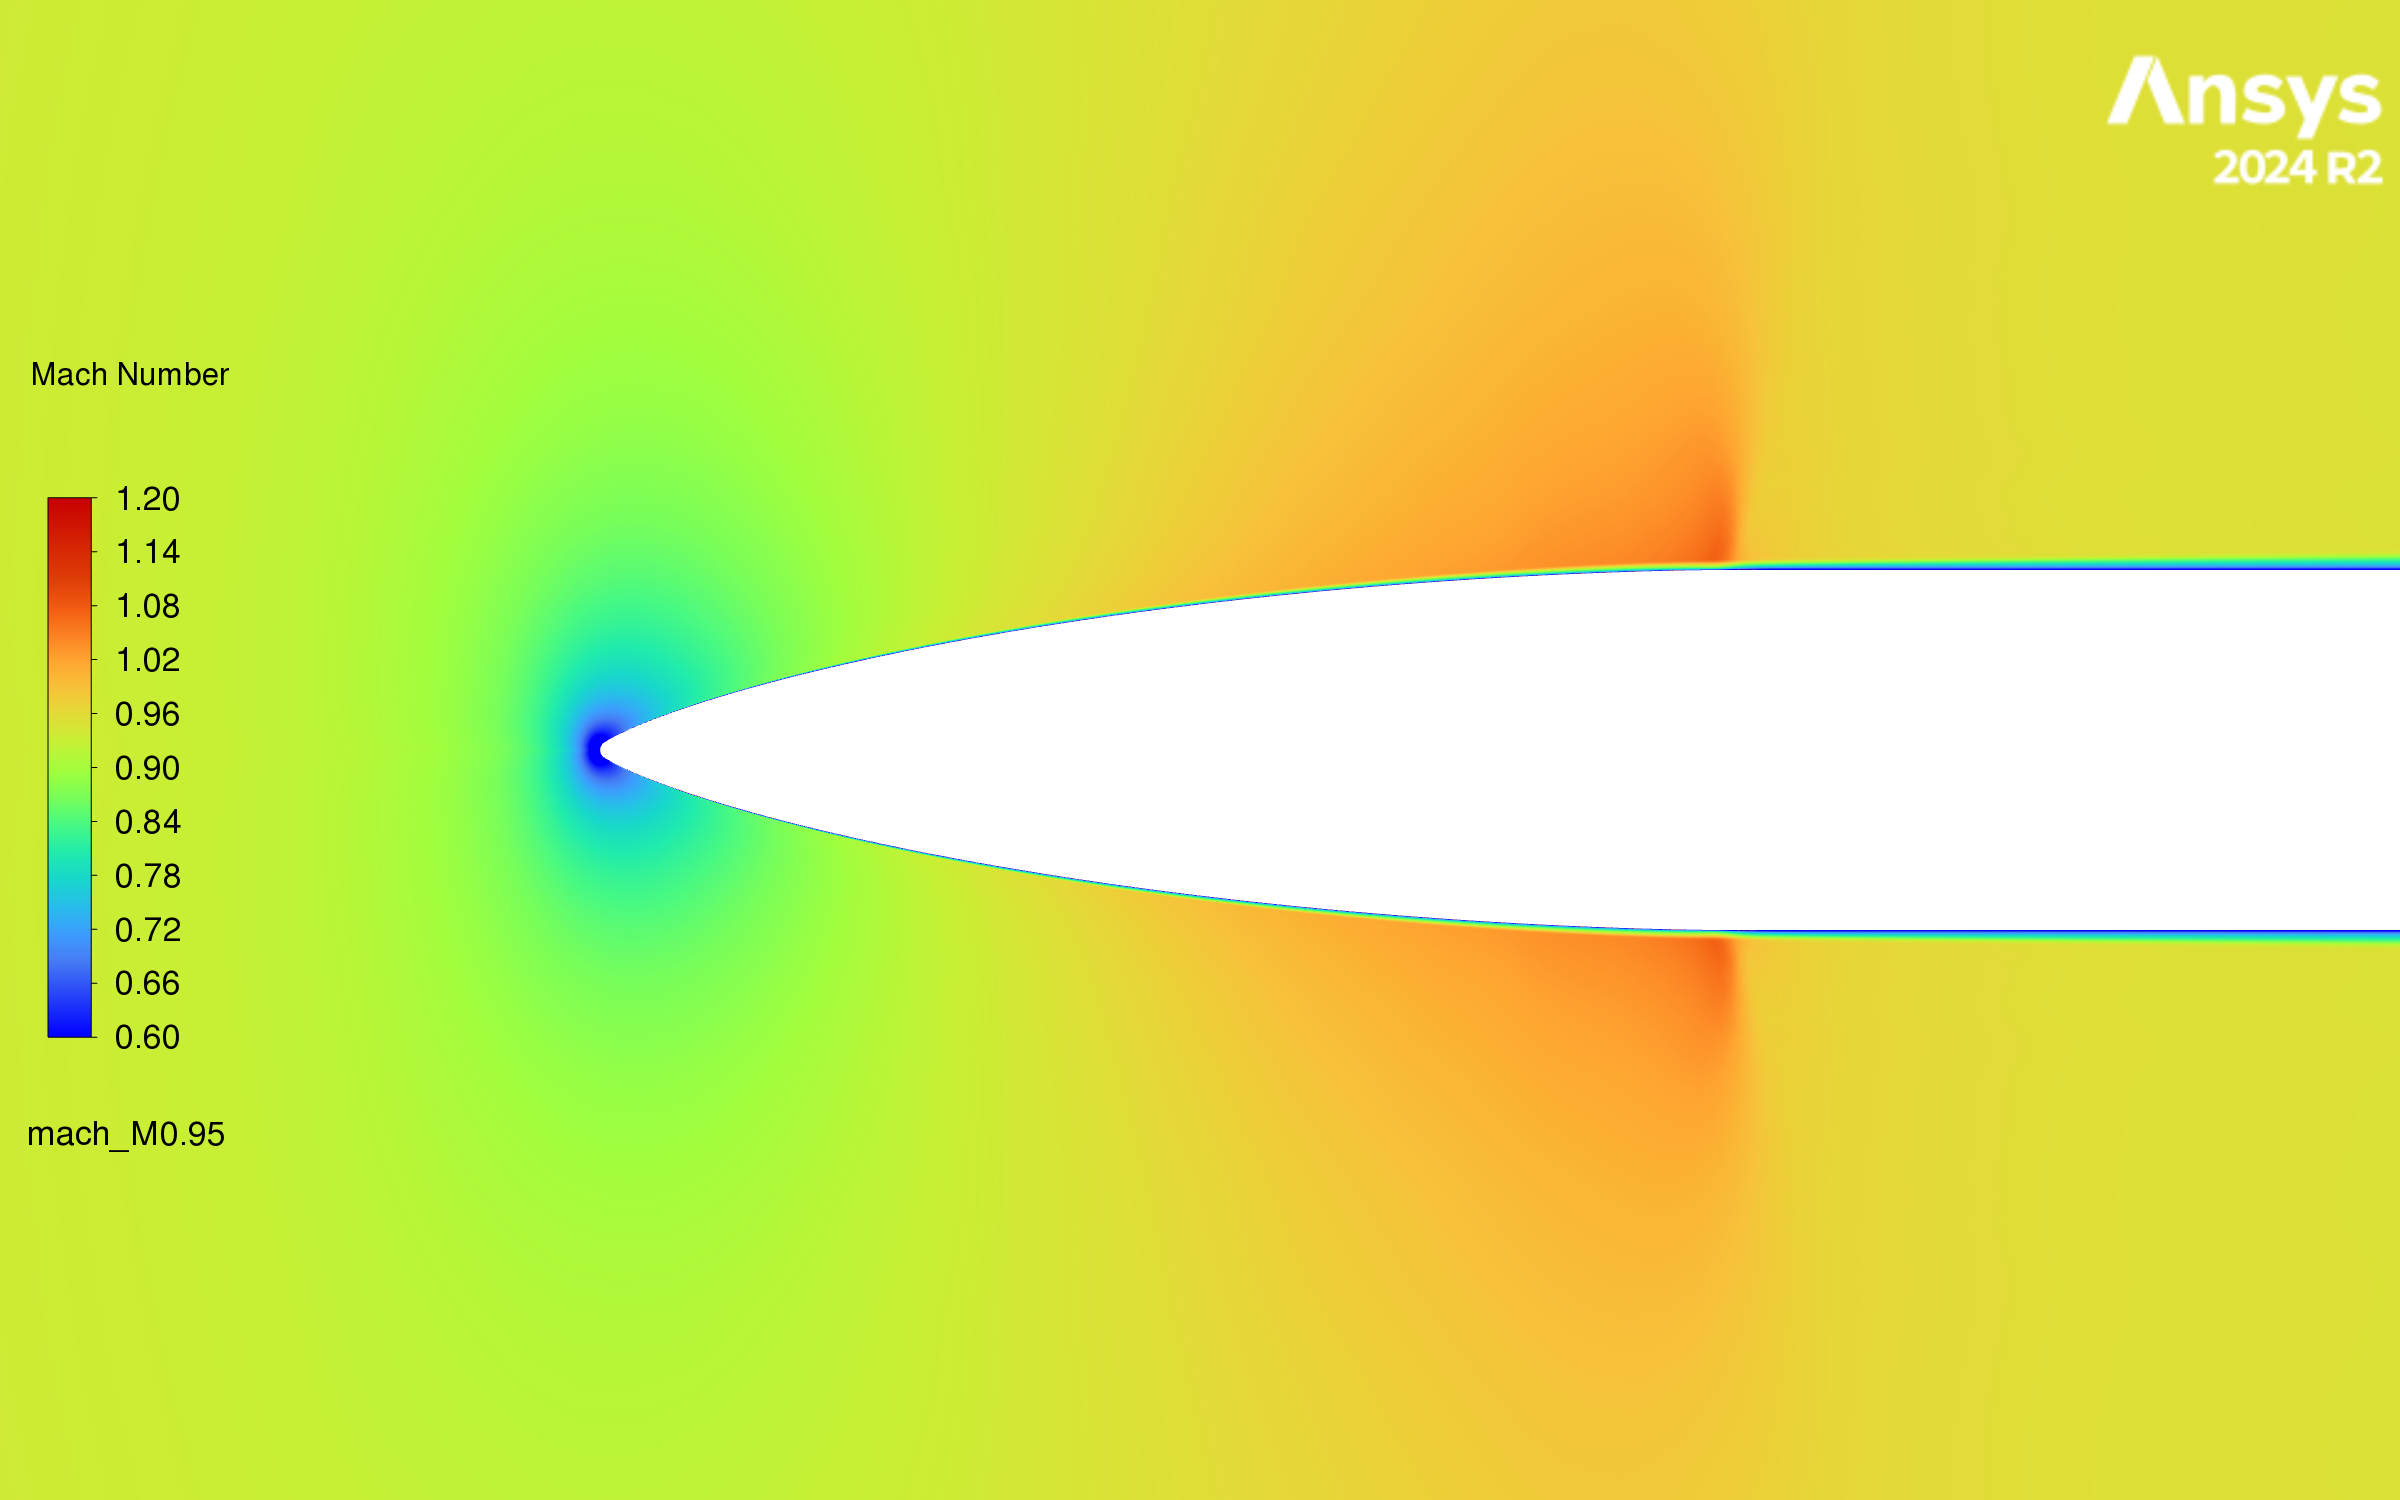
\includegraphics[width=\linewidth]{fluent_mach_M0.95}
\caption{$M = 0.95$ (0.6--1.2).}
\end{subfigure}
\caption{Mach number contours from Fluent around the nose, mirrored about the axis; each run has its own
colour scale.}
\label{fig:mach}
\end{figure}

\begin{itemize}
\item \textbf{$M = 1.47$.} The bow shock stands off the blunt tip, with subsonic flow behind it near the
axis (dark blue). It weakens outwards to $M \approx 1.3$--1.4. The flow re-expands along the nose to
$M \approx 1.55$ at the shoulder.
\item \textbf{$M = 1.2$.} Same picture; the shock stands further off and is more curved. $M \approx 1.3$
at the shoulder.
\item \textbf{$M = 0.95$.} No bow shock. The flow stagnates at the tip and accelerates along the nose; a
supersonic pocket ($M \approx 1.05$--1.1) forms at the shoulder and ends in a weak shock.
\end{itemize}

\begin{figure}[H]
\centering
\begin{subfigure}[t]{0.32\linewidth}
\centering
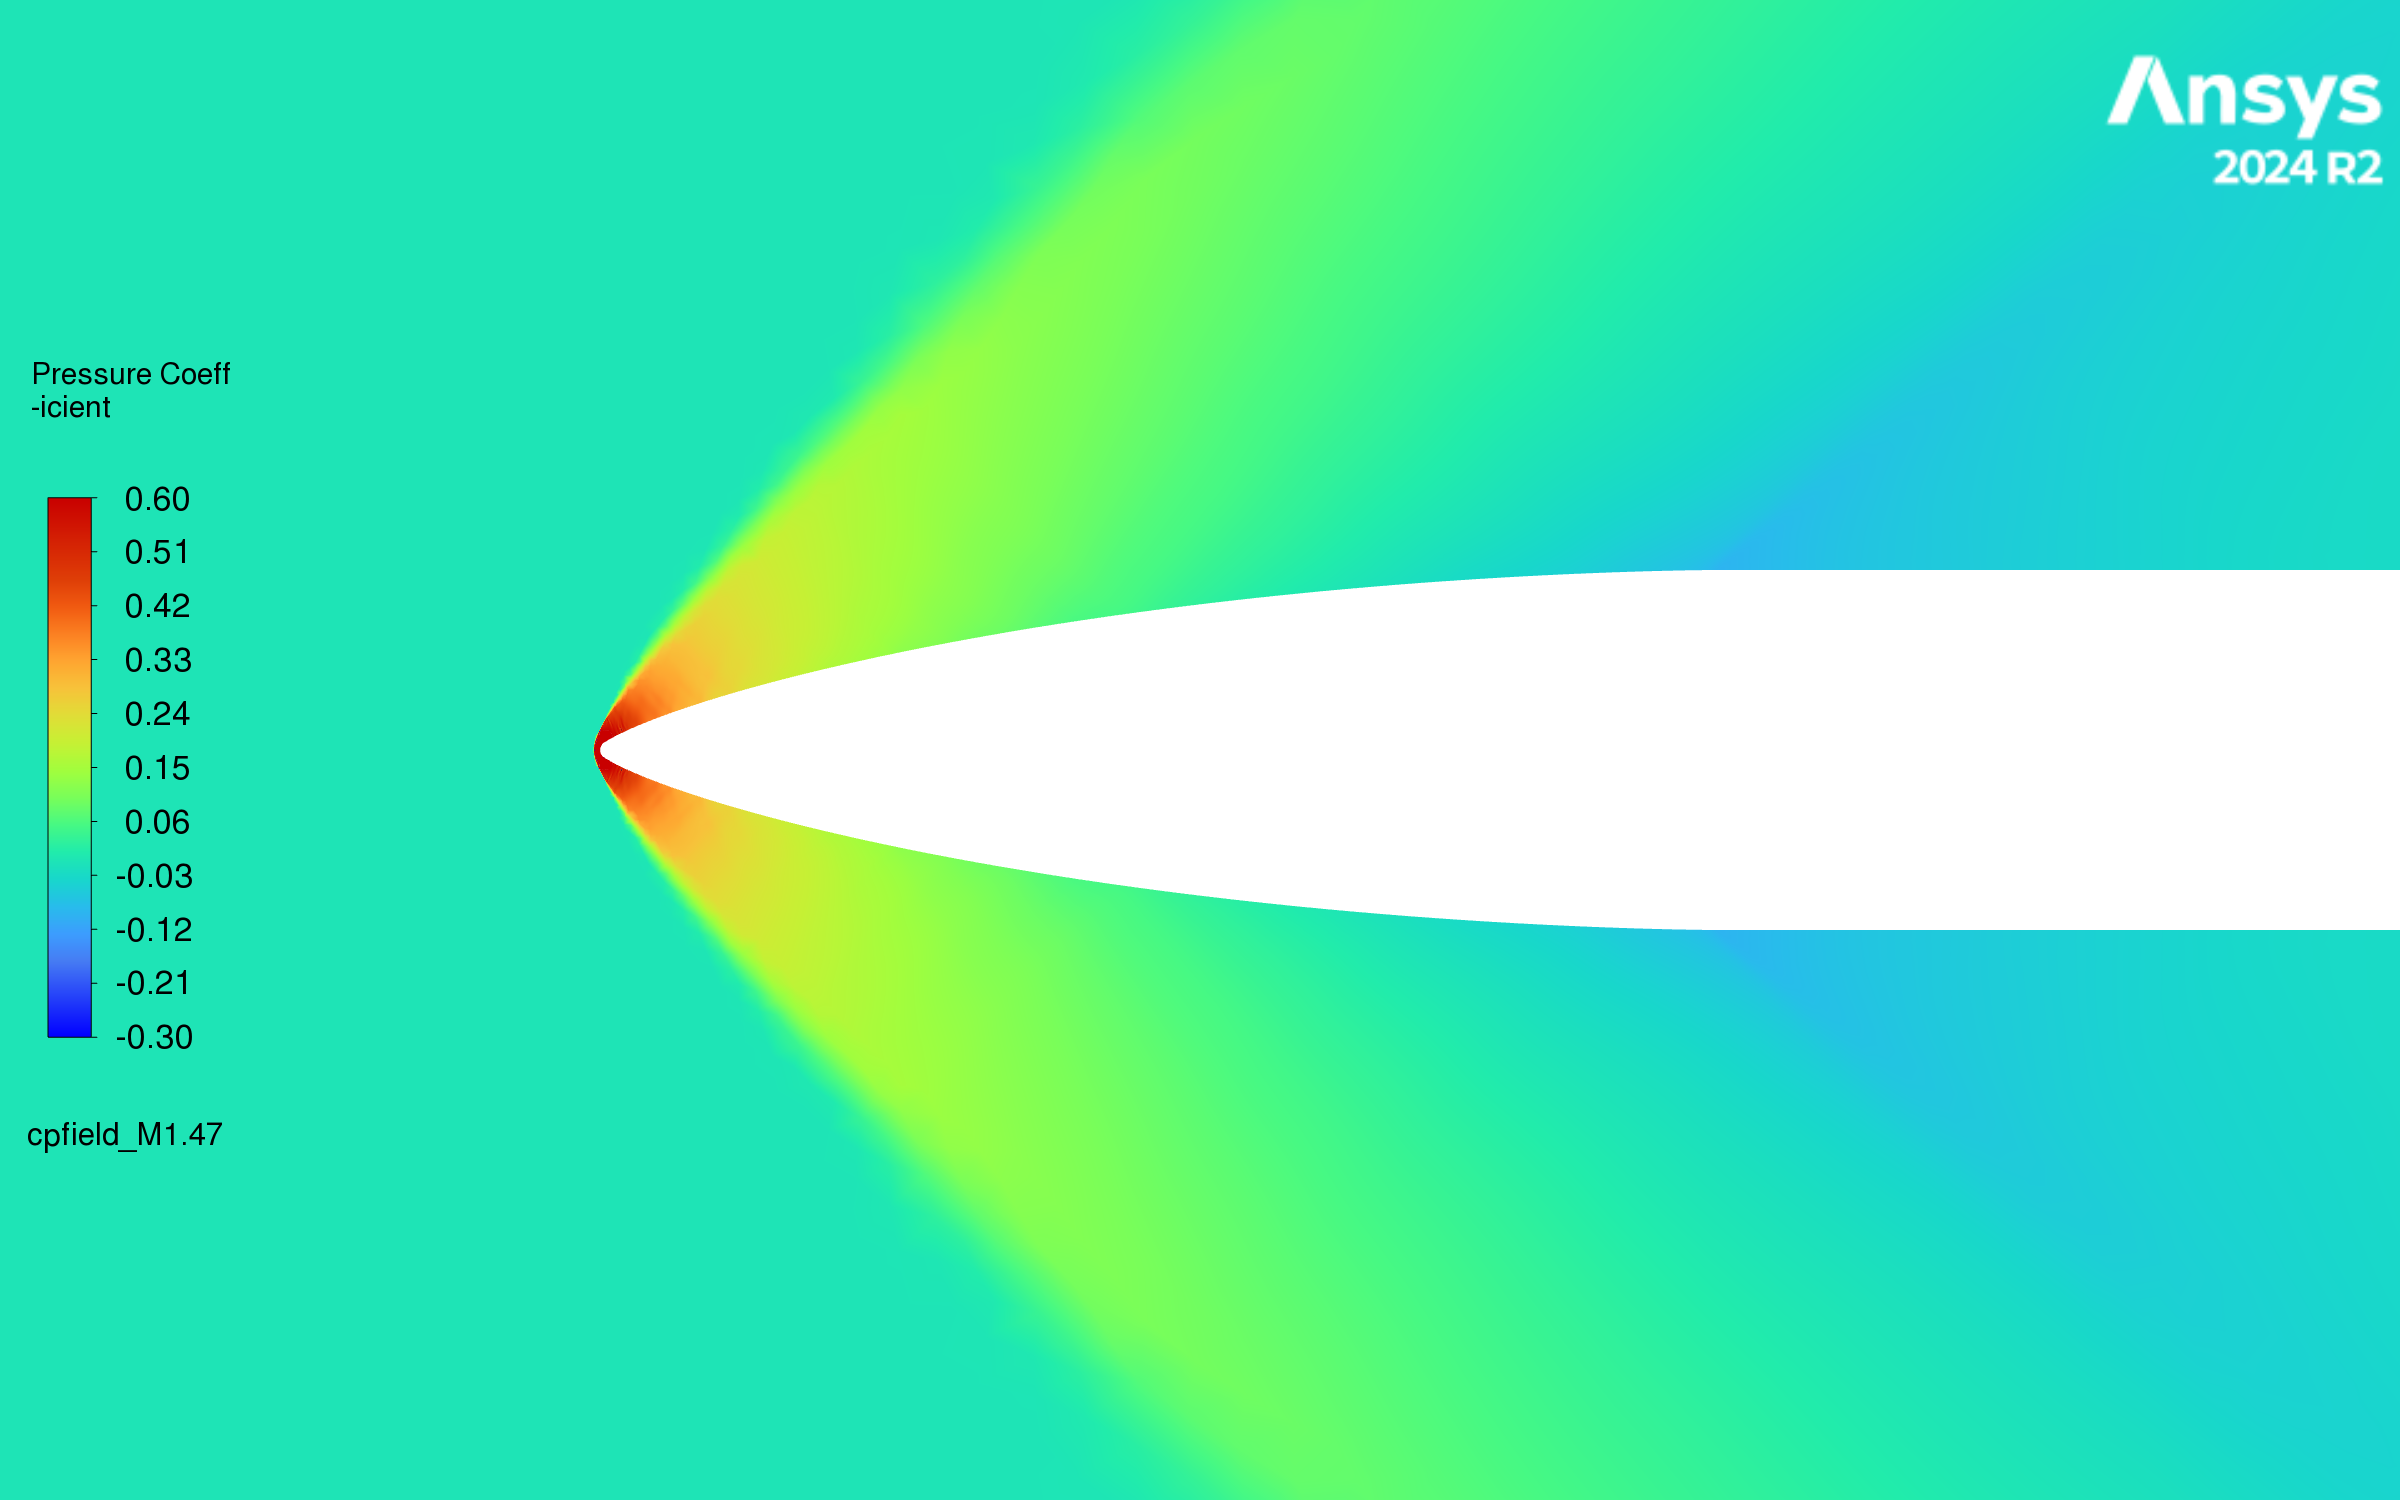
\includegraphics[width=\linewidth]{fluent_cpfield_M1.47}
\caption{$M = 1.47$.}
\end{subfigure}\hfill
\begin{subfigure}[t]{0.32\linewidth}
\centering
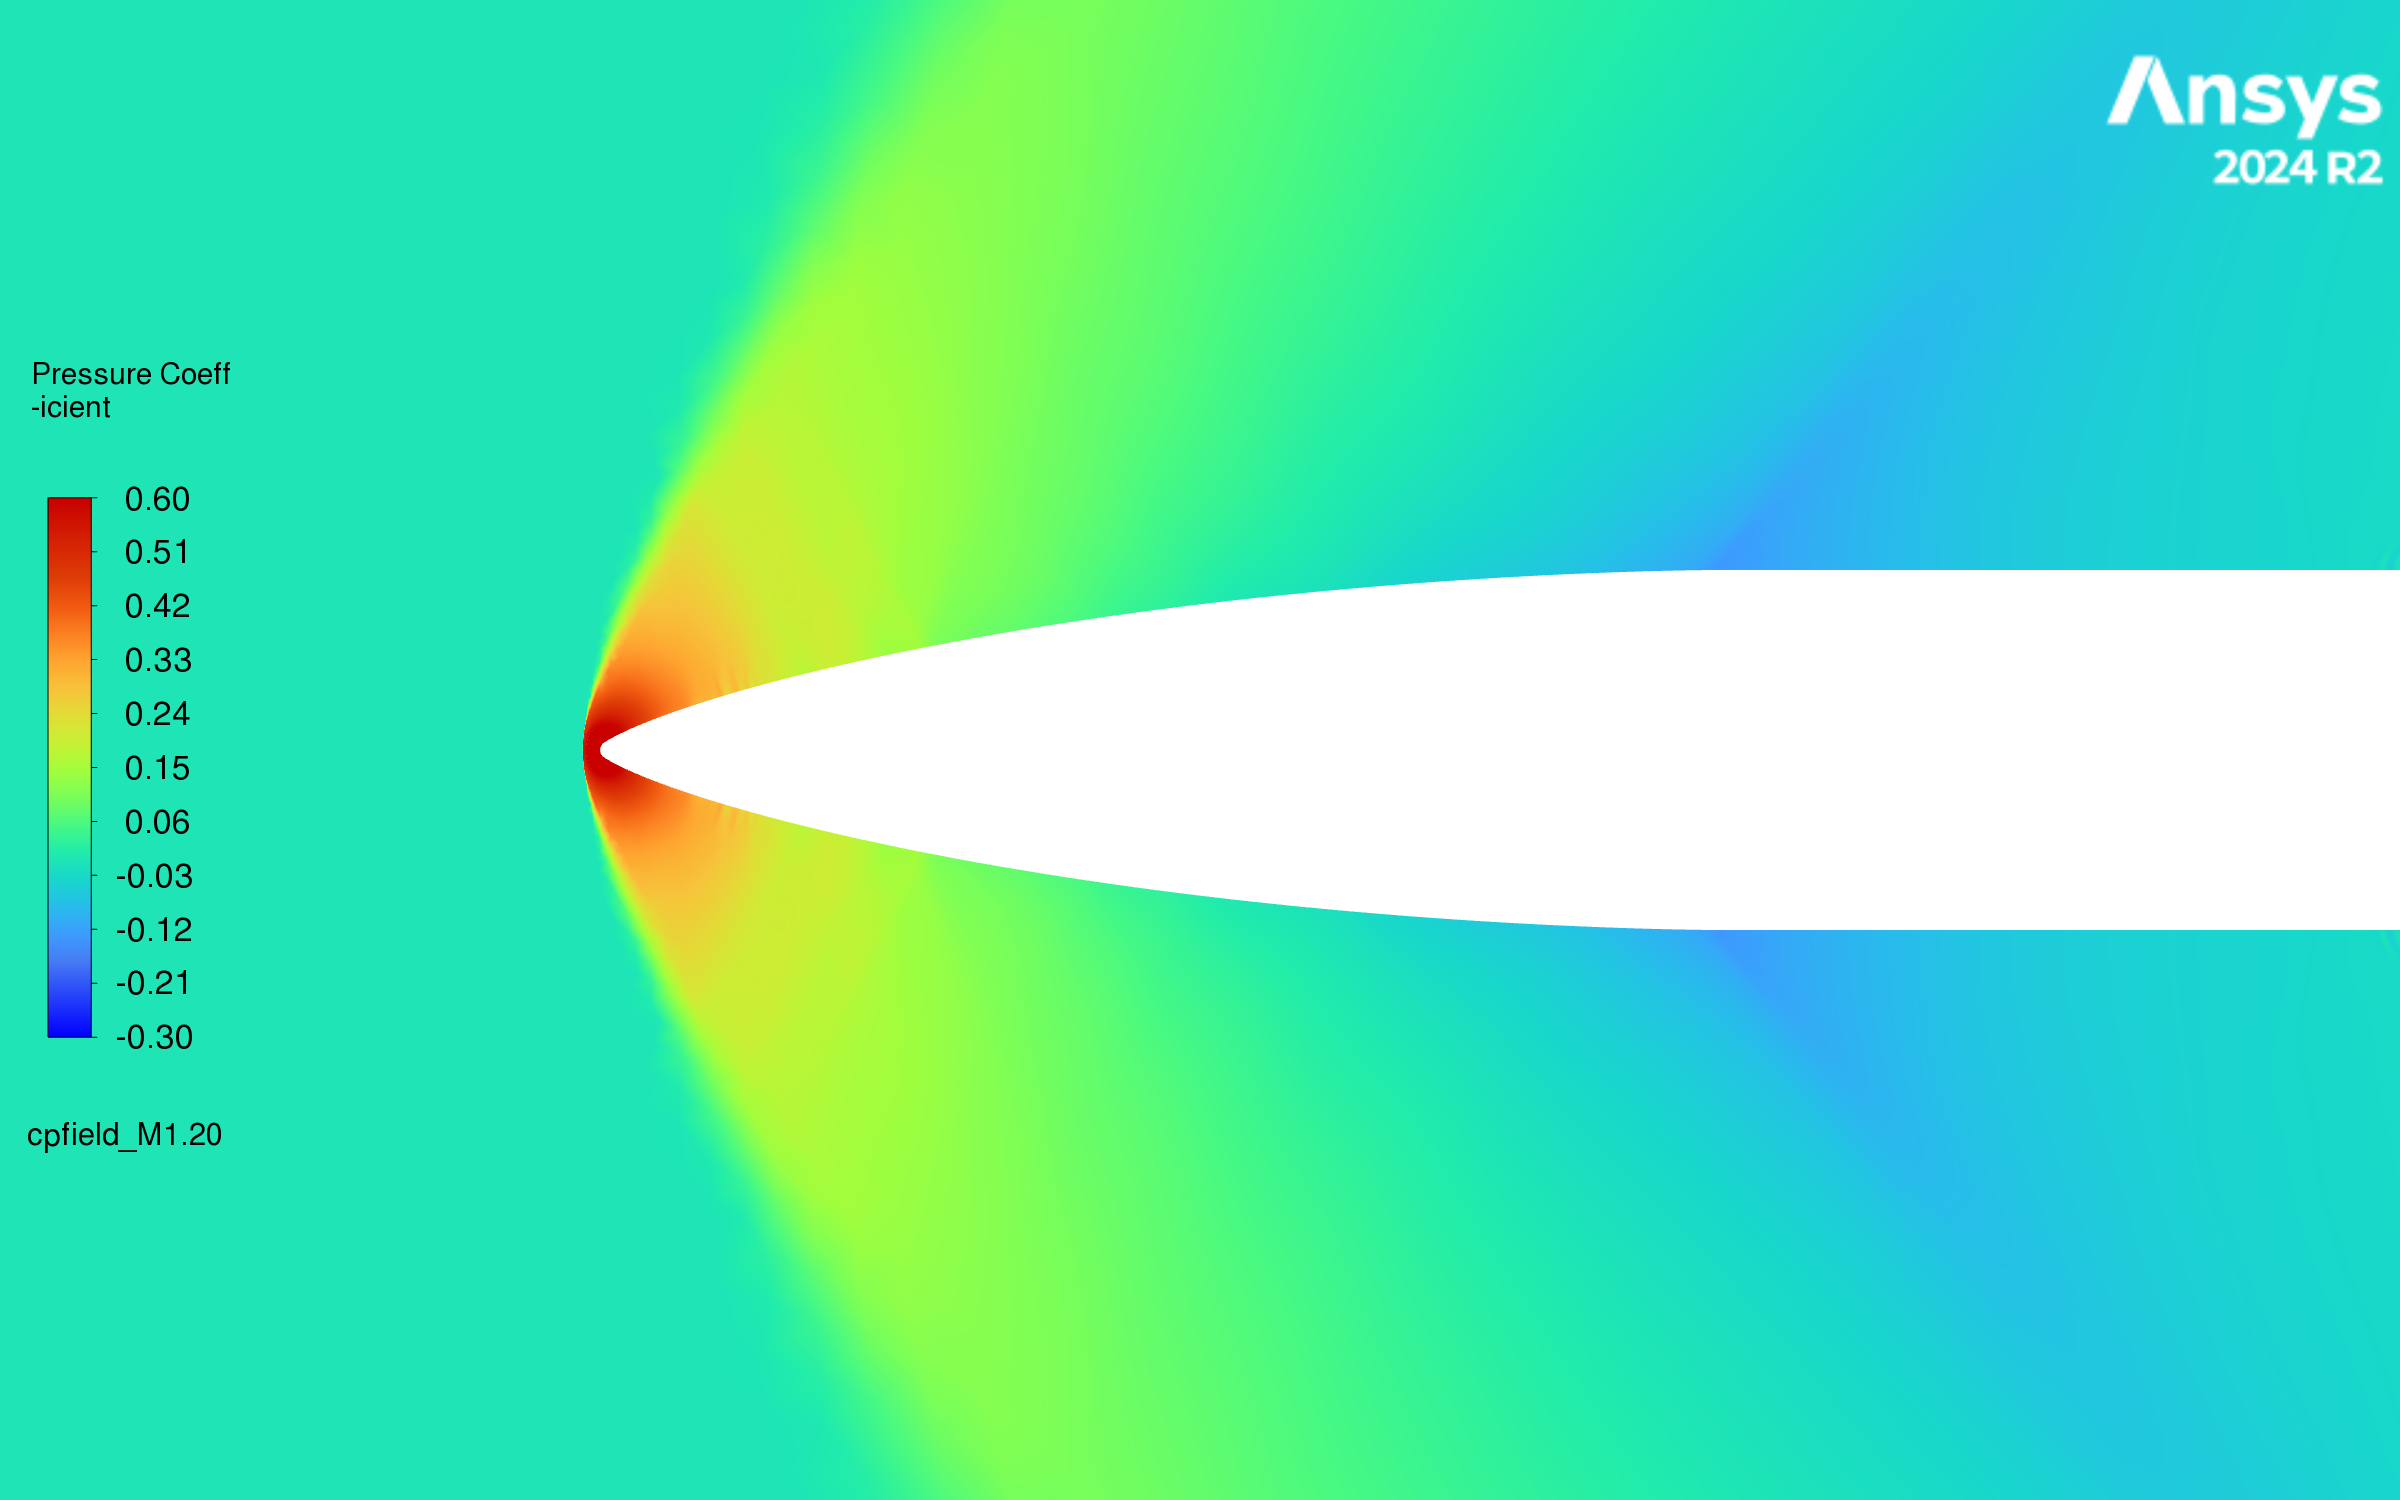
\includegraphics[width=\linewidth]{fluent_cpfield_M1.20}
\caption{$M = 1.2$.}
\end{subfigure}\hfill
\begin{subfigure}[t]{0.32\linewidth}
\centering
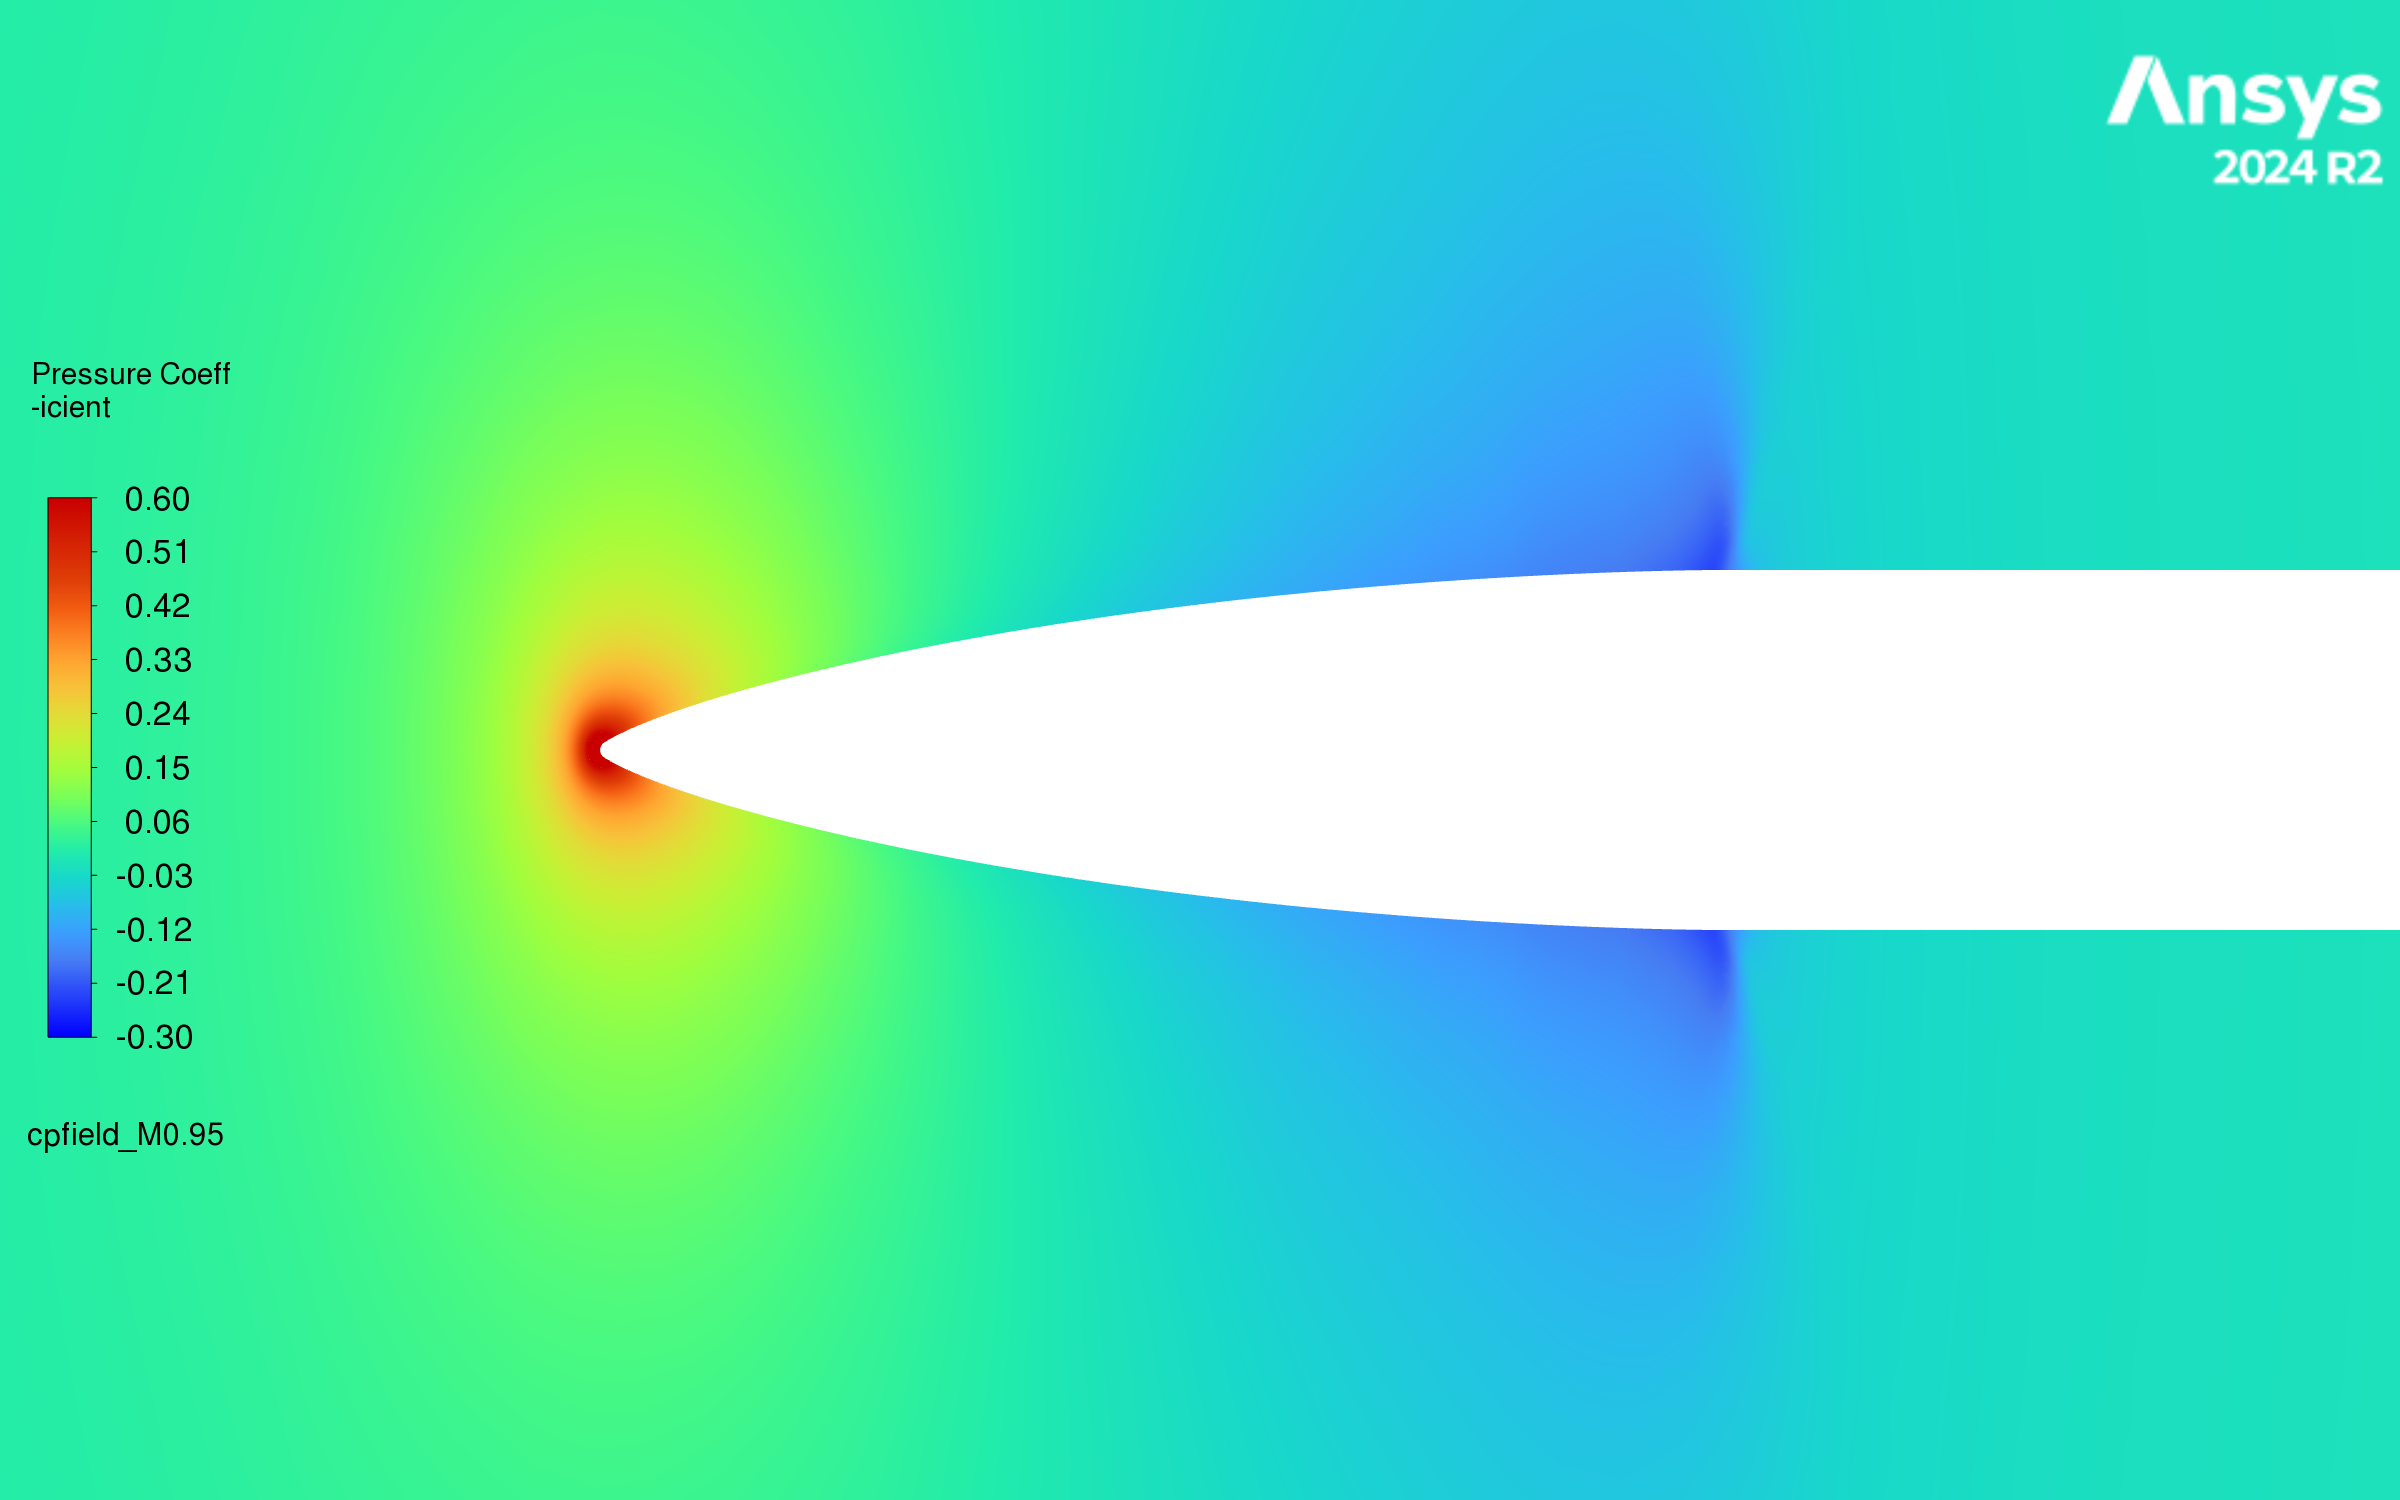
\includegraphics[width=\linewidth]{fluent_cpfield_M0.95}
\caption{$M = 0.95$.}
\end{subfigure}
\caption{Pressure coefficient $C_p = (p - p_\infty)/q_\infty$ around the nose, from Fluent, on the same
colour scale ($-0.3$ to 0.6) for all three runs.}
\label{fig:cpfield}
\end{figure}

Above $M = 1$ the high pressure behind the bow shock (red to yellow) covers the front half of the nose:
that is the wave drag. At $M = 0.95$ the high pressure stays close to the tip and the rear of the nose is
in suction (blue), so the two nearly cancel (Figure~\ref{fig:cpfield}).

\subsection{Checks}

\begin{table}[H]
\centering
\caption{Checks of the three runs.}
\label{tab:checks}
\small
\begin{tabular}{@{}lrrr@{}}
\toprule
 & $M = 0.95$ & $M = 1.2$ & $M = 1.47$ \\
\midrule
Maximum $y^+$ on \zone{wall\_nose} / \zone{wall\_body} & 0.51 / 0.28 & 0.60 / 0.30 & 0.71 / 0.29 \\
Drag force $F_x$ on \zone{wall\_nose} & \SI{42.32}{N} & \SI{254.75}{N} & \SI{349.42}{N} \\
\texttt{cd-nose} reported by Fluent & 0.0291 & 0.1172 & 0.1170 \\
$\Delta$ over the last 500 iterations & 0.009\,\% & 0.083\,\% & 0.032\,\% \\
\bottomrule
\end{tabular}
\end{table}

\begin{itemize}
\item $y^+ < 1$ on both walls at all three Mach numbers.
\item Not done yet: a mesh-independence study (Section~\ref{sec:conclusions}).
\end{itemize}

\subsection{Pressure and friction along the nose}

\begin{figure}[H]
\centering
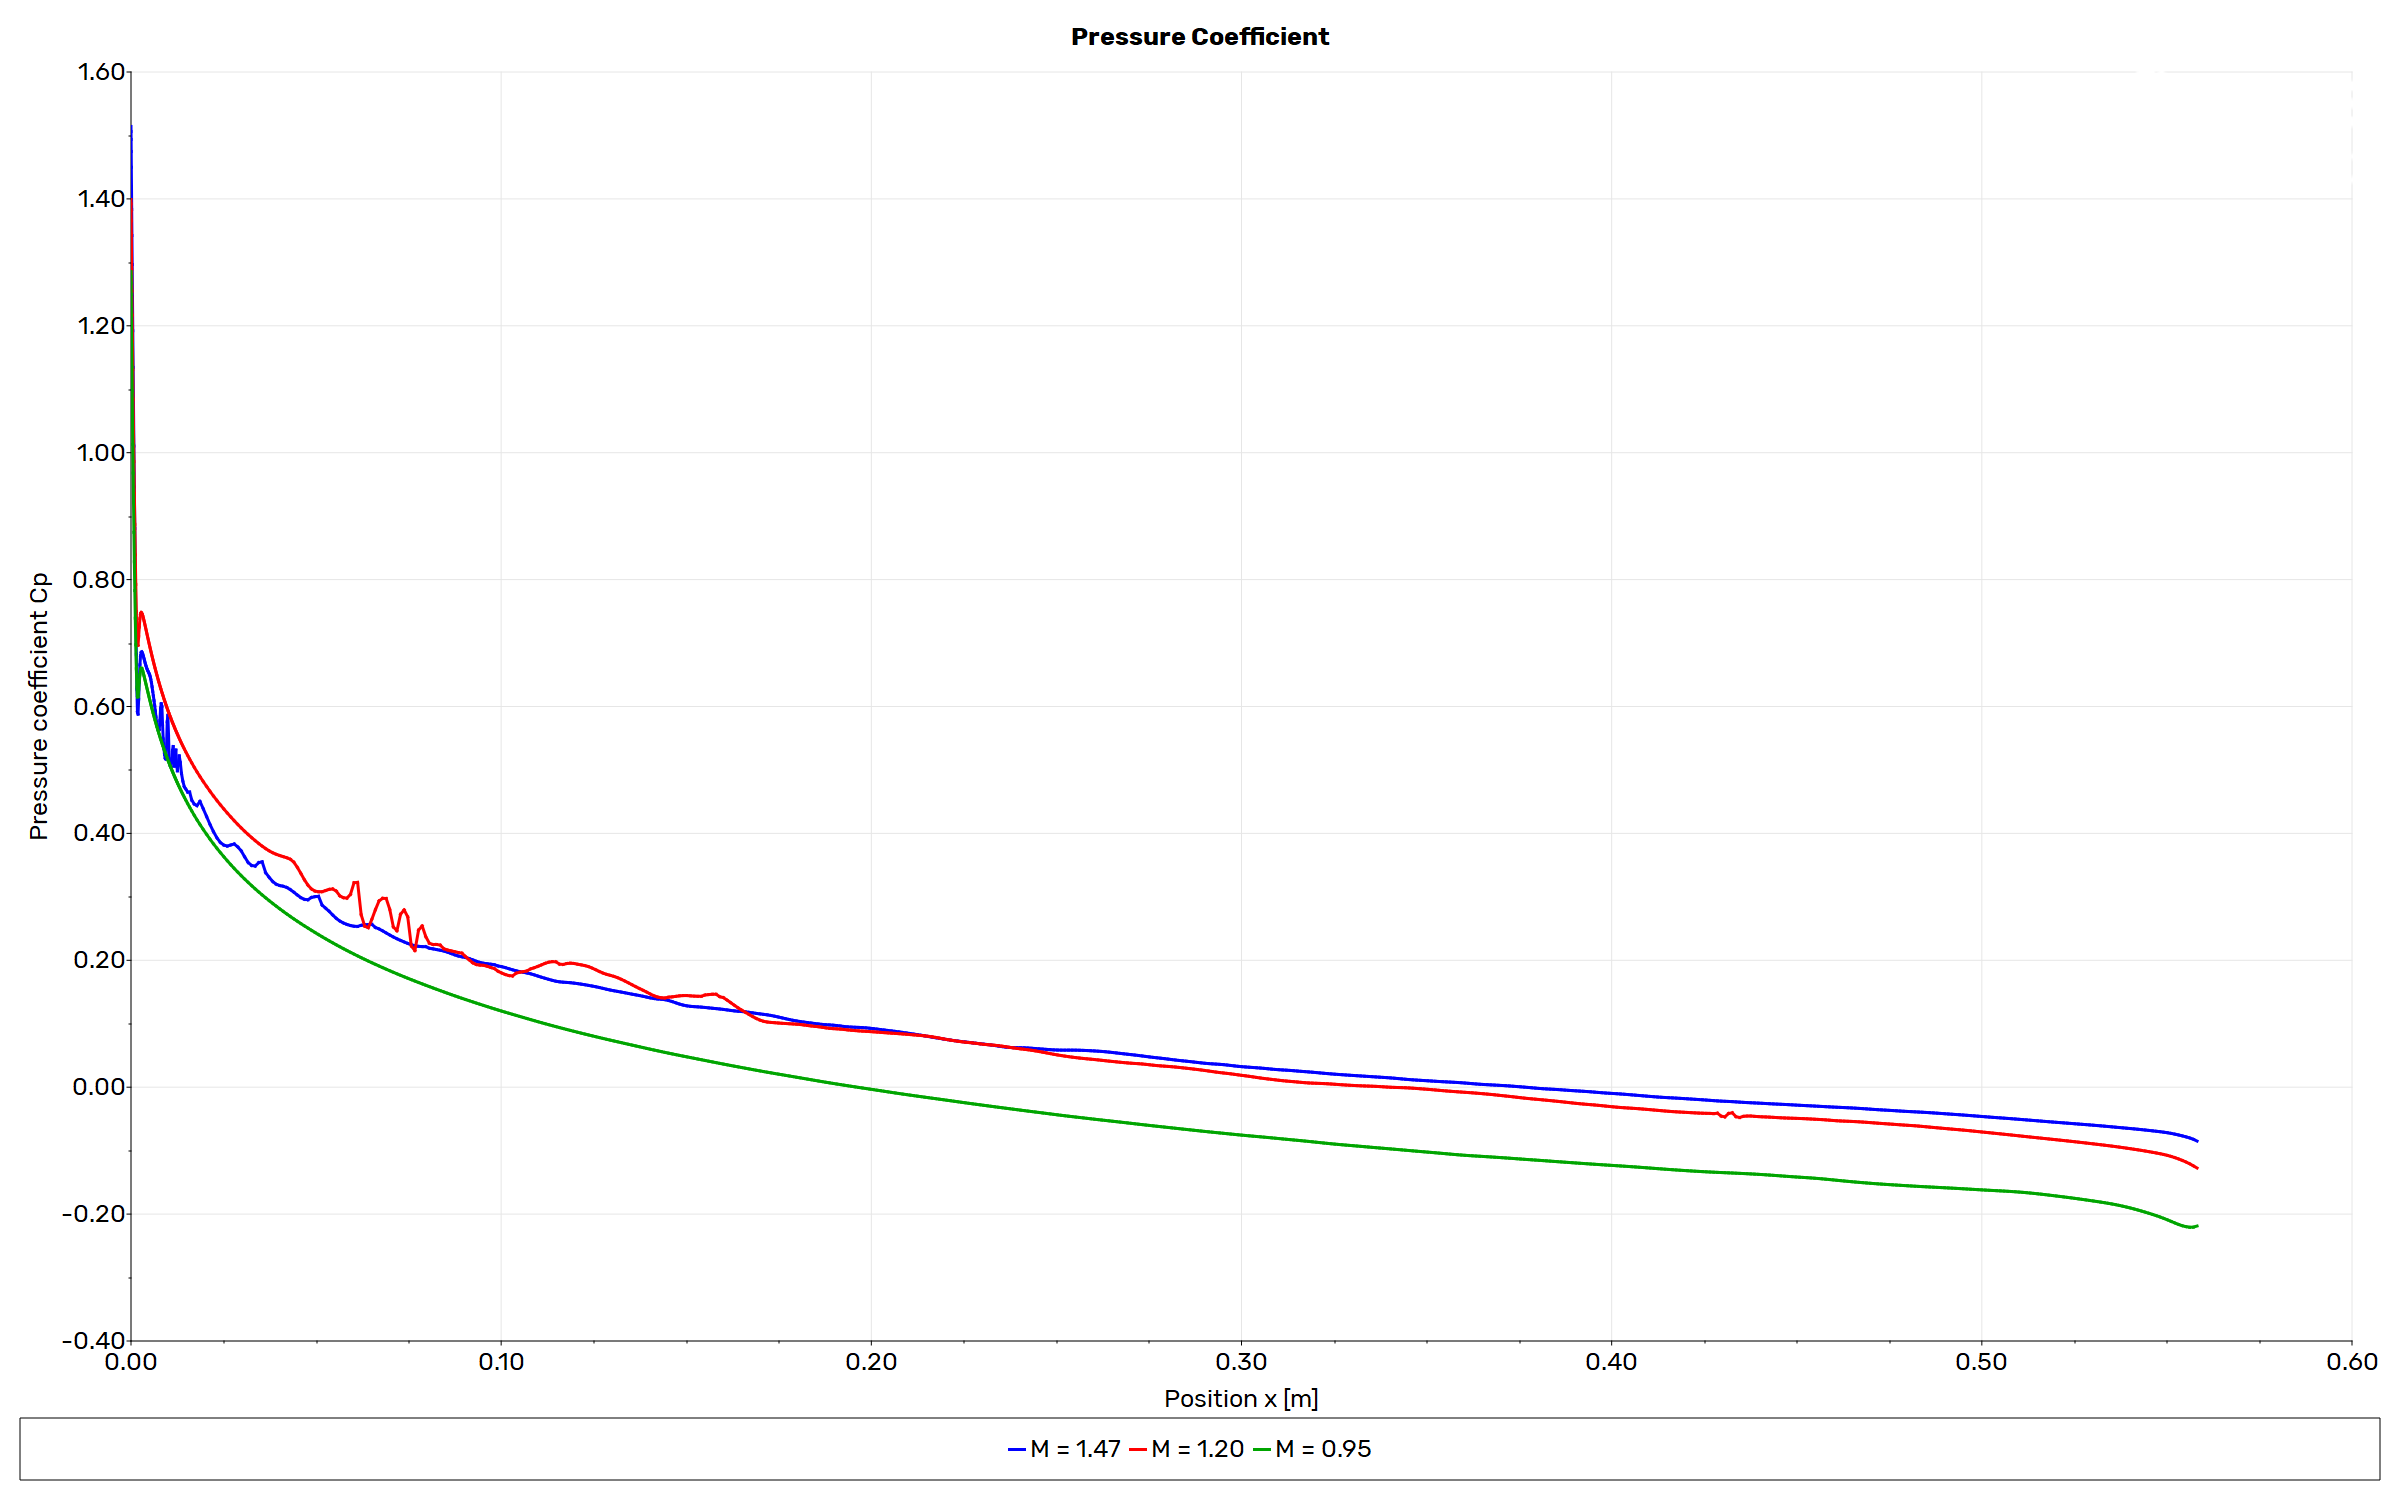
\includegraphics[width=0.9\linewidth]{fluent_cp_all}
\caption{Pressure coefficient along \zone{wall\_nose} at the three Mach numbers (Fluent XY plot).}
\label{fig:cp}
\end{figure}

\begin{figure}[H]
\centering
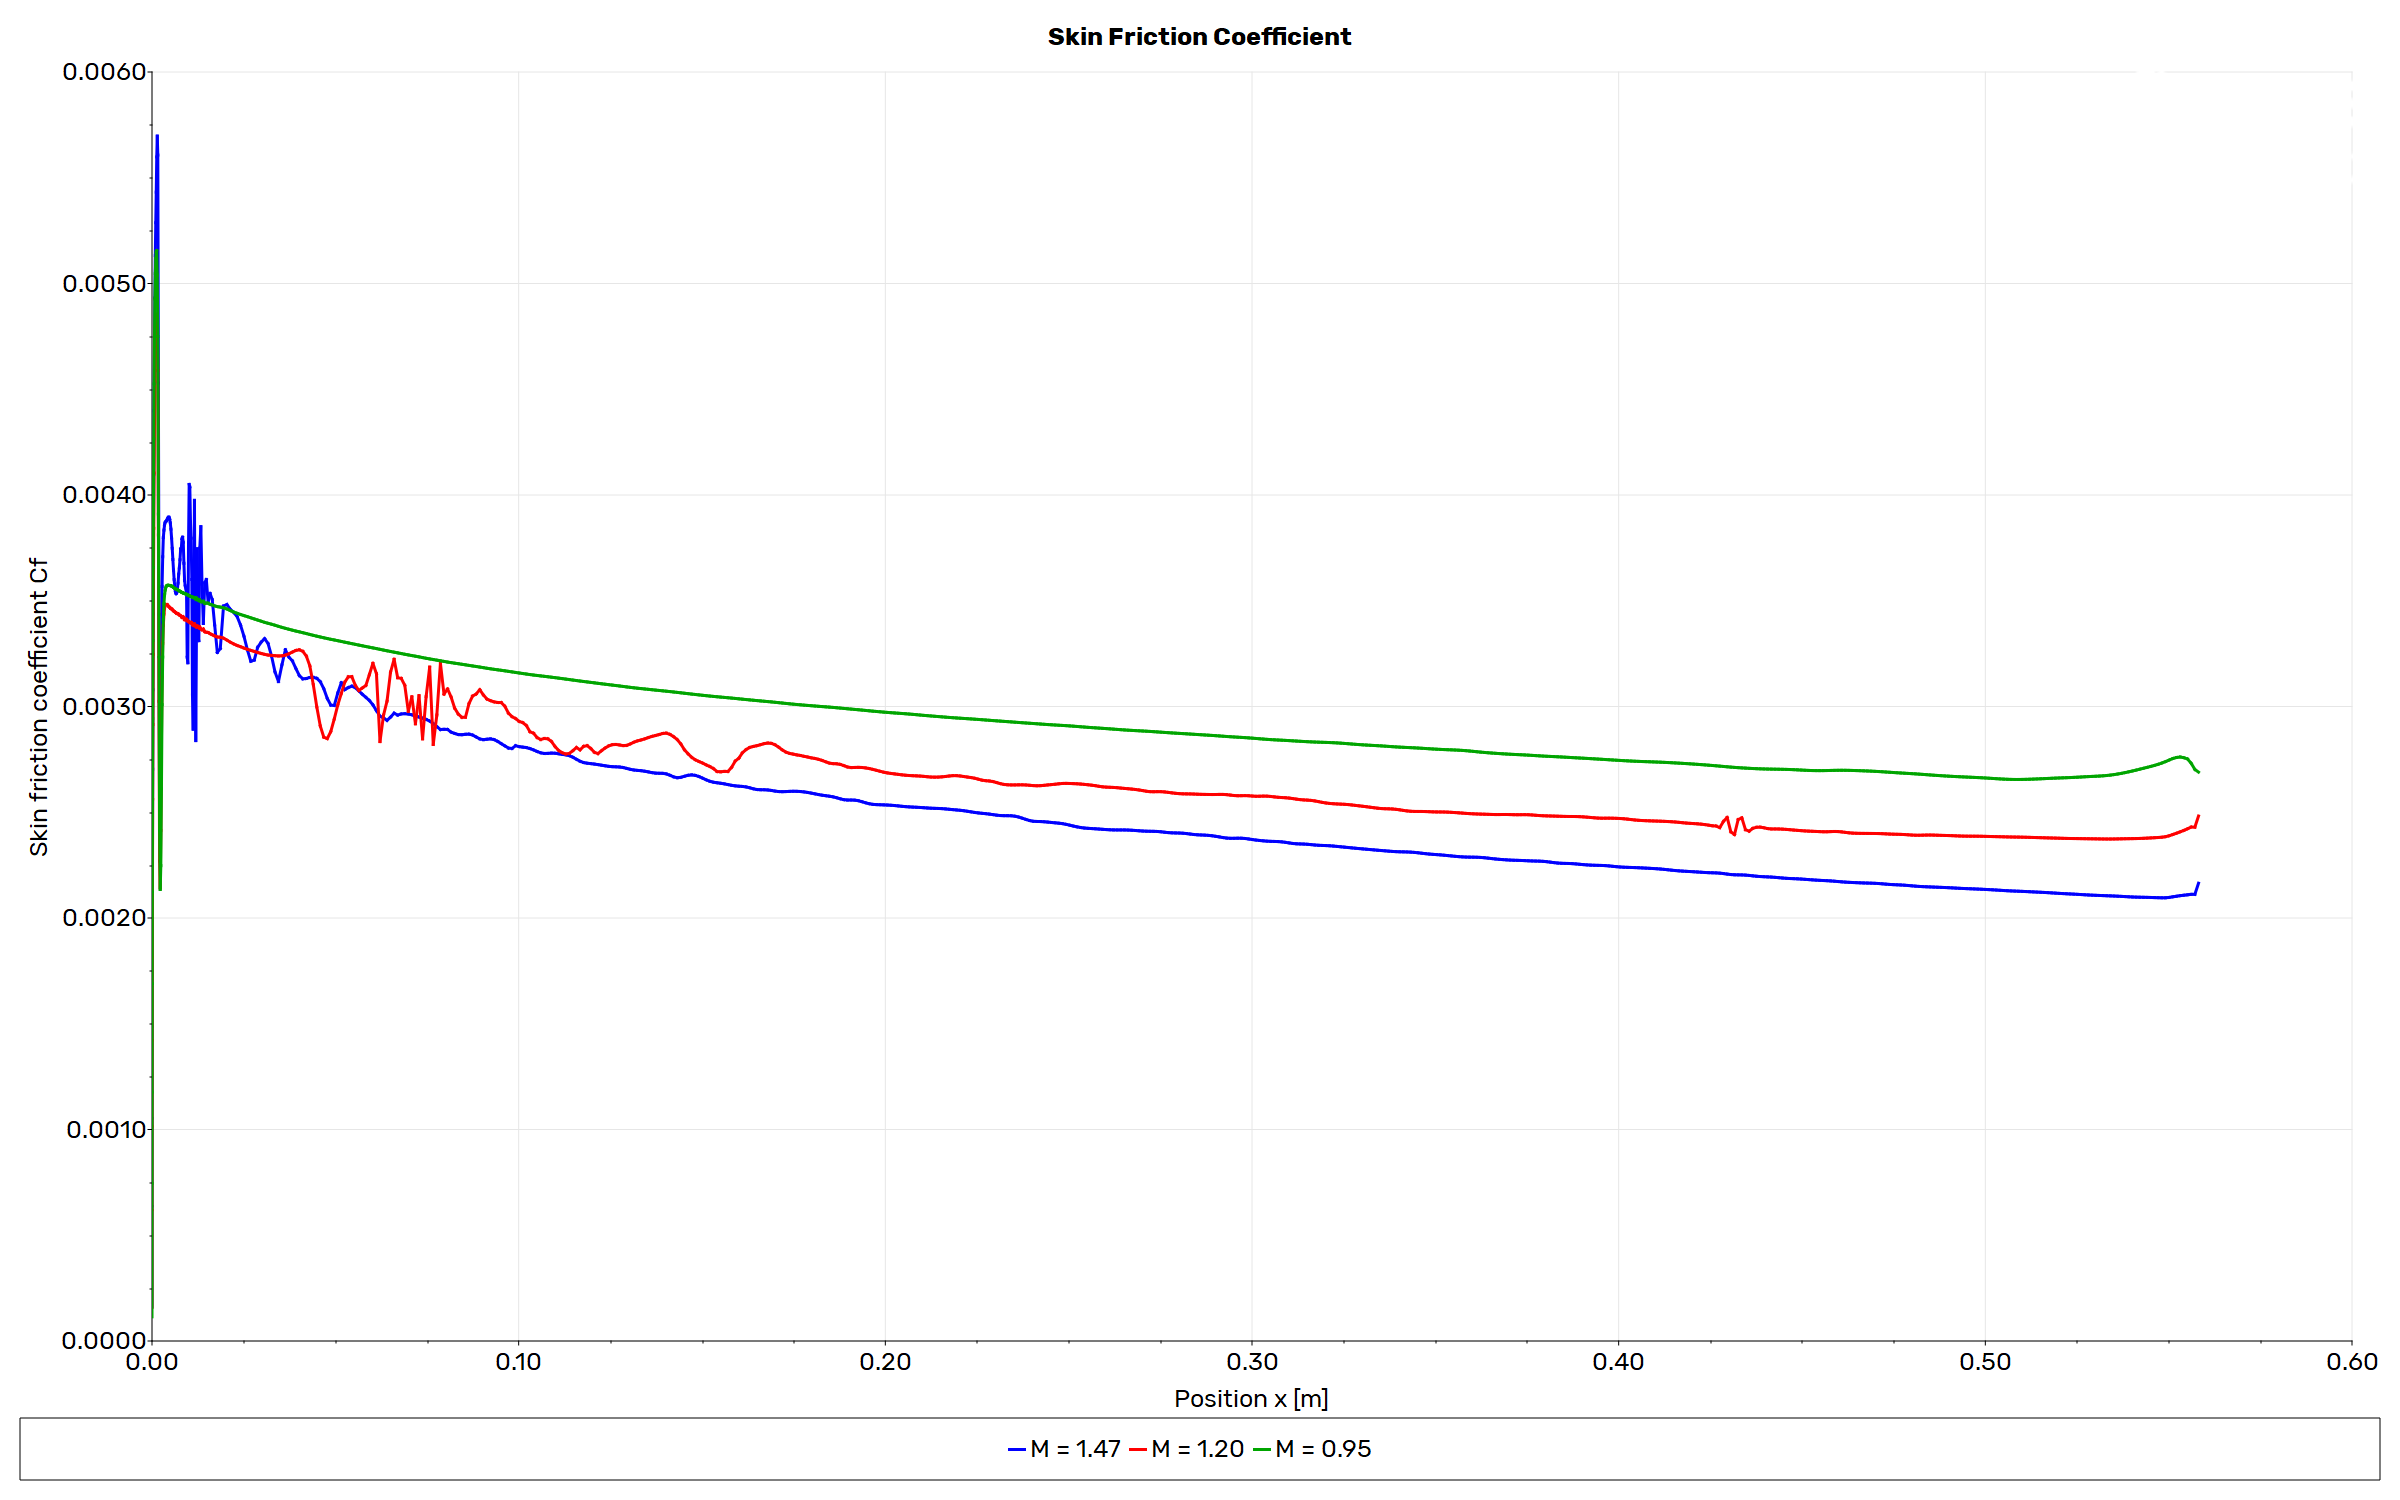
\includegraphics[width=0.9\linewidth]{fluent_cf_all}
\caption{Skin-friction coefficient along \zone{wall\_nose} at the three Mach numbers (Fluent XY plot).}
\label{fig:cf}
\end{figure}

\paragraph{Pressure (Figure~\ref{fig:cp}).} It peaks at the tip, $C_p = 1.51$ ($M = 1.47$) and 1.40
($M = 1.2$), within 0.4\,\% of the normal-shock value: the bow shock is captured correctly. Above $M = 1$
the wall stays above $p_\infty$ up to $x \approx 340$--\SI{375}{mm}: that is the wave drag. At
$M = 0.95$ it drops below $p_\infty$ at $x \approx \SI{195}{mm}$ and reaches $C_p = -0.22$ at the
shoulder, so the suction cancels most of the push on the front. The wiggles at $x = 50$--\SI{170}{mm}
($M = 1.2$) are numerical and average out.

\paragraph{Friction (Figure~\ref{fig:cf}).} Highest just behind the tip ($\approx 5\cdot10^{-3}$), it falls
to 2.2--$2.7\cdot10^{-3}$ at the shoulder as the boundary layer grows, and is lower at higher $M$.

\section{Comparison with the Python results of report 2}
\label{sec:python}

Report~2 used two nose terms from the Python tool. They are compared here with Fluent at the same free
stream and reference area.
\begin{itemize}
\item \textbf{Wave drag}: Euler simulations (no viscosity, pointed tip) interpolated to $L/D = 3.117$.
Below $M = 1.1$ there were no Euler runs, so the tool uses an assumed ramp:
\begin{equation}
C_{D,w}(M) = C_{D,w}(1.1)\; s^2(3 - 2s), \qquad s = \frac{M - 0.8}{0.2}\ \text{clipped to } [0, 1].
\end{equation}
Compared with Fluent's pressure part.
\item \textbf{Friction}: turbulent flat plate on the nose alone, smooth wall:
\begin{equation}
C_f = \frac{0.455}{(\log_{10}\mathrm{Re}_L)^{2.58}} \times
\begin{cases} 1 - 0.1M^2, & M < 1,\\ (1 + 0.15M^2)^{-0.58}, & M > 1, \end{cases}
\qquad C_{D,f} = C_f\,\frac{S_{\rm wet}}{A_{\rm ref}}, \quad S_{\rm wet} = \SI{0.2243}{m^2}.
\end{equation}
Compared with Fluent's viscous part.
\end{itemize}

\begin{table}[H]
\centering
\caption{Nose drag of study~A: Python (report~2) and Fluent. Difference = Fluent / Python $-$ 1.}
\label{tab:python}
\small
\begin{tabular}{@{}lrrrrrr@{}}
\toprule
 & \multicolumn{3}{c}{pressure (wave) $C_D$} & \multicolumn{3}{c}{friction (viscous) $C_D$} \\
\cmidrule(lr){2-4}\cmidrule(l){5-7}
$M$ & Python & Fluent & difference & Python & Fluent & difference \\
\midrule
0.95 & 0.0768 & 0.0042 & $-94.5$\,\% & 0.0236 & 0.0248 & $+5.2$\,\% \\
1.2 & 0.0926 & 0.0948 & $+2.4$\,\% & 0.0225 & 0.0224 & $-0.5$\,\% \\
1.47 & 0.0941 & 0.0963 & $+2.4$\,\% & 0.0210 & 0.0207 & $-1.4$\,\% \\
\bottomrule
\end{tabular}

\end{table}

\begin{figure}[H]
\centering
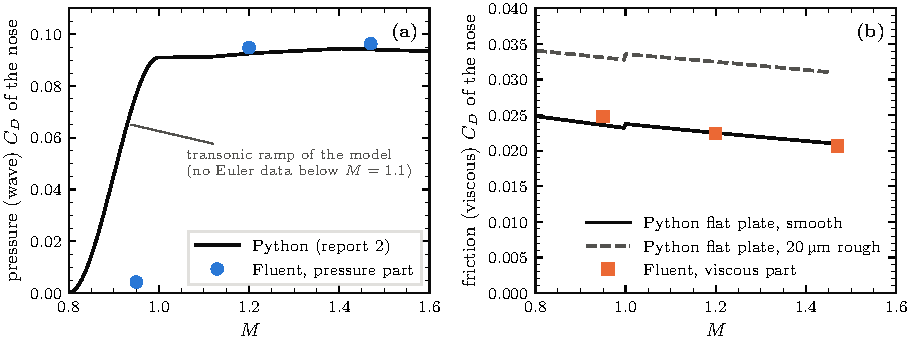
\includegraphics[width=\linewidth]{fig_python_compare}
\caption{(a) Wave drag of the Python model against Mach, and Fluent's pressure part. (b) Python
flat-plate friction of the nose along the boost of the report-2 trajectory (the Reynolds number changes
with $M$), for a smooth wall and for the \SI{20}{\micro m} roughness of the trajectory model, and
Fluent's viscous part. The small step at $M = 1$ is where the Python formula switches from its
subsonic to its supersonic compressibility correction.}
\label{fig:python}
\end{figure}

\paragraph{Supersonic: $+2.4\,\%$ at both Mach numbers.} Fluent has the real \SI{4.5}{mm} rounded tip and a
boundary layer that makes the nose act slightly fatter; both add a little pressure drag. With the
sensitivity of report~2 ($\approx\SI{7}{m}$ of apogee per per cent of wave drag), $+2.4\,\%$ costs about
\SI{17}{m}.

\paragraph{Friction: within $-1.4\,\%$ to $+5.2\,\%$.} The flat plate models the nose friction well. The
\SI{20}{\micro m} roughness of the trajectory model adds 40--47\,\% (dashed line), which these smooth-wall
runs do not check.

\paragraph{Transonic: Python is conservative.} At $M = 0.95$ the ramp gives 0.0768 ($s = 0.75$, so
84\,\% of the $M = 1.1$ value); Fluent gives 0.0042. The drag rise comes later and steeper than assumed,
so the drag of report~2 is too high between $M \approx 0.8$ and 1.0 and its apogee is on the safe side.
Placing the rise needs a Fluent run at $M = 1.0$--1.1 (Section~\ref{sec:conclusions}).

\section{Conclusions and next runs}
\label{sec:conclusions}

\begin{itemize}
\item Converged drag: $C_D = 0.0291$ / 0.1172 / 0.1170 at $M = 0.95$ / 1.2 / 1.47, with $y^+ < 1$ and
$\Delta < 0.1\,\%$ in every run.
\item The mesh is within the Ansys limits: skewness 0.92, orthogonal quality 0.237 (Meshing) / 0.077
(Fluent).
\item Supersonic runs: density-based solver. Transonic run: pressure-based Coupled with Viscous Heating.
\item Against Python: wave drag $+2.4\,\%$, friction within 5\,\%; the transonic ramp is conservative below
$M = 1$.
\end{itemize}

\paragraph{Next runs, in order of priority.}
\begin{enumerate}
\item \textbf{Mesh independence} at $M = 1.47$: coarse and fine mesh ($\times1.5$ per direction each step),
plus 1--2 pressure-gradient adaptions at the shock.
\item \textbf{Transonic rise}: $M = 1.05$ (pressure-based) and $M = 1.1$.
\item \textbf{Solver cross-check}: $M = 1.2$ with the pressure-based solver.
\item \textbf{Backflow temperature}: one run with $T_0$ instead of $T_\infty$.
\item \textbf{Free-stream turbulence}: one run at $I = 0.1\,\%$, $\mu_t/\mu = 1$.
\item \textbf{Study B} (Von K\'arm\'an 630 + \SI{20}{mm}): same steps; pull the coupler end from
$x = \SI{645.42}{mm}$ to \SI{2447.65}{mm}.
\item \textbf{Incidence}: 3D half model at \SI{5}{\degree} for $C_{N\alpha}$ and the centre of pressure
($y^+ \approx 30$--50 is enough there).
\end{enumerate}


\clearpage
\appendix
\section{Files}
\label{app:files}

\paragraph{In the repository} (\file{weisshorn-nose-cone}, paths from its root):

\begin{table}[H]
\centering
\small
\begin{tabularx}{\linewidth}{@{}>{\raggedright\arraybackslash}p{7.4cm}>{\raggedright\arraybackslash}X@{}}
\toprule
File & Contents \\
\midrule
\file{CFD/geometry_650/nose_lvhaack_L561_c89_rn4.5mm.step}, \file{.csv} & Study-A design solid and profile points \\
\file{CFD/geometry_650/nose_vonkarman_L630_c20_rn4.5mm.step}, \file{.csv} & Study-B design solid and profile points \\
\file{CFD/geometry_650/studyA_domain2D_2024R2.dsco} & Study-A 2D flow domain (Discovery 2024~R2) \\
\file{CFD/studyA/README.md}, \file{studyA_log.html} & Run log of study~A \\
\file{CFD/studyA/freestream_bc.py} & Free stream, boundary values, first-cell height and $C_D$ from the forces \\
\file{CFD/studyA/cd_history/*.csv} & $C_D$ on \zone{wall\_nose} per iteration, all four runs \\
\file{CFD/studyA/plots/*.png} & Fluent pictures: $C_D$, residuals, Mach contours \\
\file{CFD/studyA/report_figures.py} & Figures of this report and the comparison with report~2 \\
\file{CFD/mcp/} & Claude Code + Fluent MCP set-up for the DLL remote PCs (Appendix~\ref{app:claude}) \\
\file{CFD/source/} & Source of this report \\
\bottomrule
\end{tabularx}
\end{table}

\section{Driving Fluent from Claude Code on the DLL remote PCs}
\label{app:claude}

The study-A runs were driven by Claude Code through an MCP server connected to the running Fluent
session. This is optional: every step of this report can be done in the Fluent GUI. The set-up is in
\file{CFD/mcp/} and follows 2026\_C\_FD\_REPORT-2\_MCP-FLUENT, with two differences: the MCP server is
\file{CFD/mcp/server.py} of this repository (the guide does not give the URL of its own), and the
Claude Code home is moved to the network drive with the \texttt{CLAUDE\_CONFIG\_DIR} variable, because
the guide's junction cannot point to a network drive.

\paragraph{Set-up, every session.}
\begin{enumerate}
\item Put the repository in the Documents folder of the network home, which survives the reset of
\texttt{C:\textbackslash} (clone it from there, or download the branch as a ZIP from GitHub).
\item In a normal PowerShell window run
\begin{center}
\small\texttt{powershell -ExecutionPolicy Bypass -File <repo>\textbackslash CFD\textbackslash mcp\textbackslash bootstrap-vm.ps1}
\end{center}
Each step is skipped when its result is already there: the first run takes about 10 minutes, later runs
seconds. It finds the newest Fluent installation and Python, installs PyFluent 0.43 and \texttt{mcp} 2.x
from the wheel cache on the network drive, installs or restores Claude Code, writes \file{.mcp.json}
(without a BOM) and starts Claude Code in the repository.
\item Start Fluent yourself (Workbench or the Fluent launcher, working directory \file{CFD/runs}). In
its console type \texttt{define/beta-feature-access} (answer yes), then \texttt{server/start-server}.
Fluent 2024~R2 refuses \texttt{start-server} until the beta features are on. Fluent writes a
\file{server_info*.txt} file.
\item Ask Claude Code to connect to that file (\texttt{connect\_to\_fluent}). The \texttt{launch\_fluent}
tool can also start a new session, but it always picks the newest installed version (2026~R1 on these
PCs), not 2024~R2.
\end{enumerate}

\paragraph{Restarting.}
\begin{itemize}
\item \textbf{Claude Code only:} type \texttt{/exit}, then run the setup script again, or start it by hand
with \texttt{claude --continue} from the repository folder. \texttt{--continue} reopens the last
conversation; inside Claude Code, \texttt{/resume} picks an older one. The history is kept on the network
drive, so it survives the restart. Fluent can stay open.
\item \textbf{MCP connection only:} type \texttt{/mcp}, choose \texttt{fluent} and \gui{Reconnect}.
Then ask Claude to run \texttt{connect\_to\_fluent} again, with the \file{CFD/runs} folder. PyFluent takes up to a
minute to load.
\item \textbf{Fluent restarted:} type \texttt{server/start-server} again in the new Fluent console, then
reconnect. Each Fluent session writes its own \file{server_info} file, and Claude uses the newest one in
the folder.
\end{itemize}

\paragraph{Tools.} The server offers 13 tools. Session: \texttt{launch\_fluent},
\texttt{connect\_to\_fluent}, \texttt{exit\_fluent}. Files: \texttt{read\_case},
\texttt{read\_case\_and\_data}, \texttt{write\_data}. Solver: \texttt{initialize}, \texttt{iterate},
\texttt{execute\_tui}, \texttt{scheme\_eval}. Reports: \texttt{get\_case\_summary},
\texttt{get\_residuals\_summary}, \texttt{screenshot}. The tool time-out is set to one hour so that
long \texttt{iterate} calls finish.

\paragraph{Things to know.}
\begin{itemize}
\item The server drives the solver only; geometry and meshing stay manual.
\item Console commands with keyword menus are easy to get wrong. Let Claude Code run iterations and read
results, but enter boundary values in the panels and check them with \texttt{/file/write-bc}.
\item One \texttt{iterate} call hung with Fluent waiting at its ``number of iterations'' prompt;
\texttt{/solve/iterate n} through \texttt{execute\_tui} works.
\item The copy of Claude Code on the PC is a separate installation: it starts without the context of
the sessions on a laptop, so give it the case description (this report) at the start.
\end{itemize}


\end{document}
